% !TEX root=./report.tex

\newpage

\section{Appendix}
\label{sec:appendix}
To declutter the report we moved many of the plots in this section.
Please see the next pages for the plots.

\begin{figure*}[!ht]
  \centering
    \begin{tabular}{cc}
      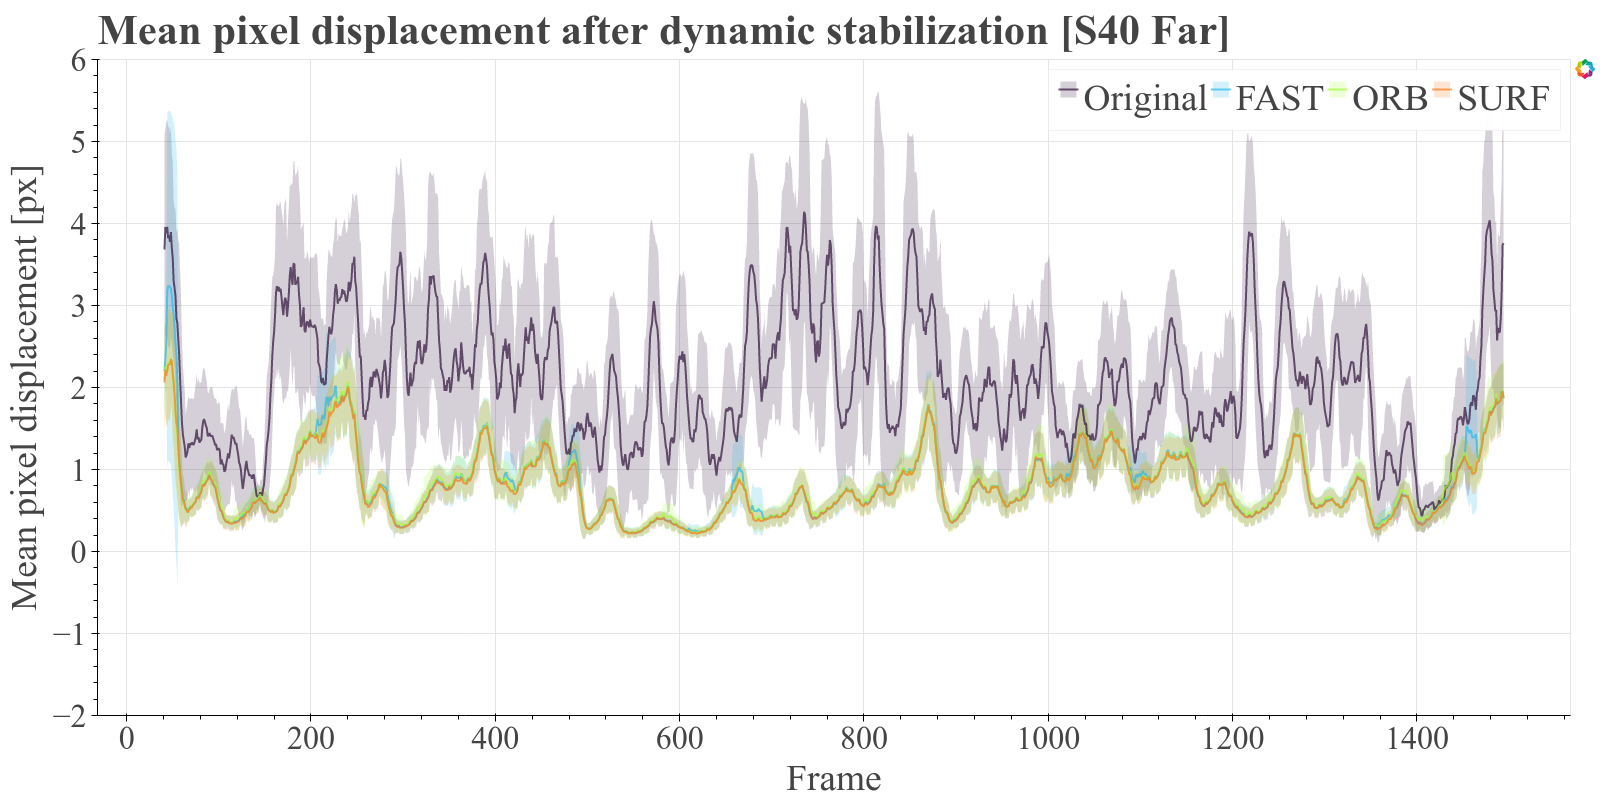
\includegraphics[width=0.475\linewidth]{diagrams/optical_flow/s40_n_far_image_raw.mp4.csv/compare_of_mean_pixel_displacement/window_size_12.html.png}    &  
      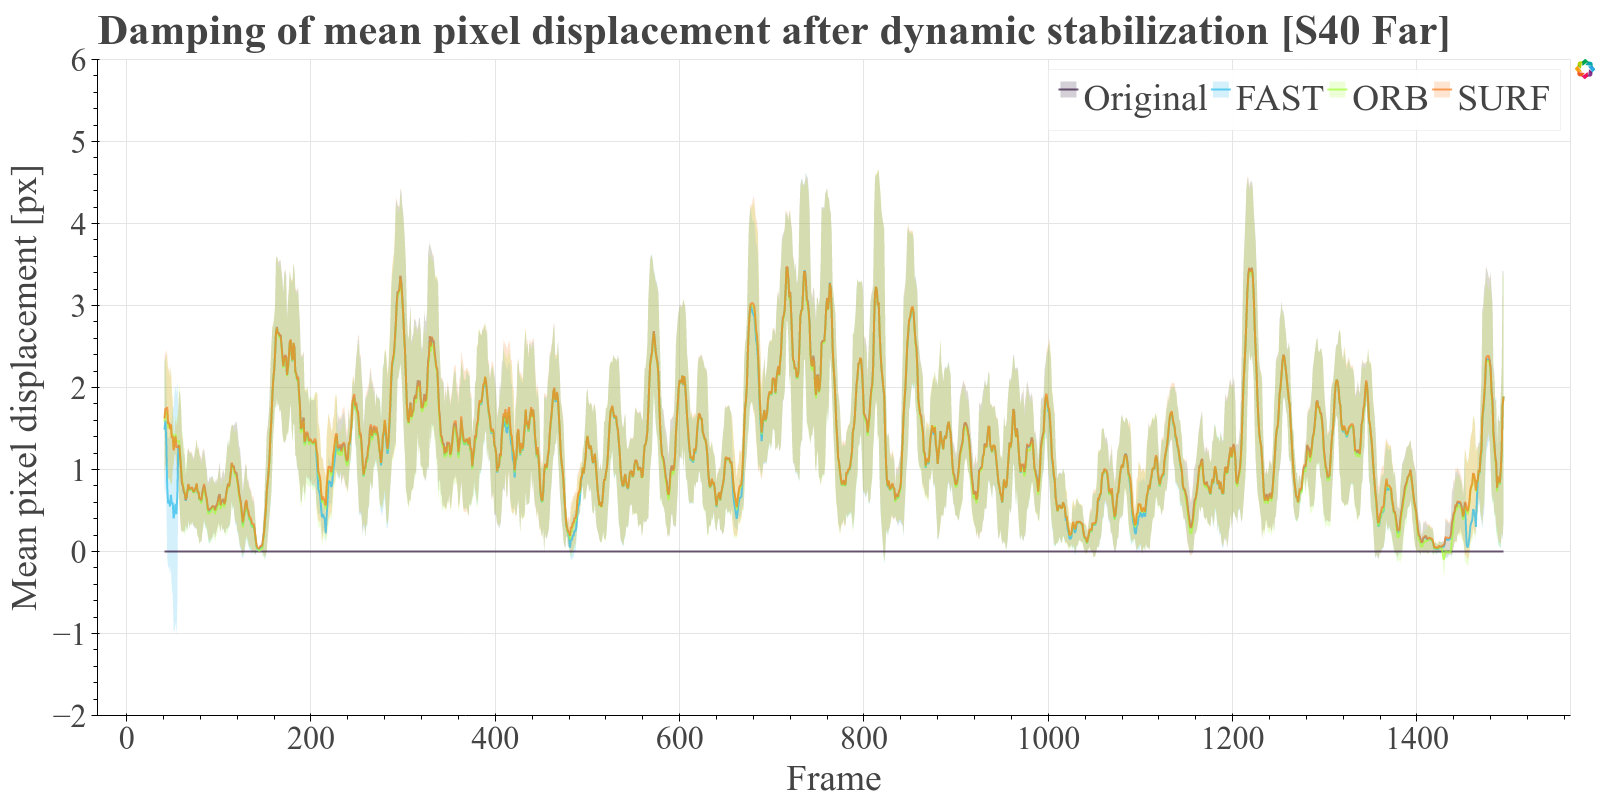
\includegraphics[width=0.475\linewidth]{diagrams/optical_flow/s40_n_far_image_raw.mp4.csv/deltas_of_mean_pixel_displacement/window_size_12.html.png}   \\ 

      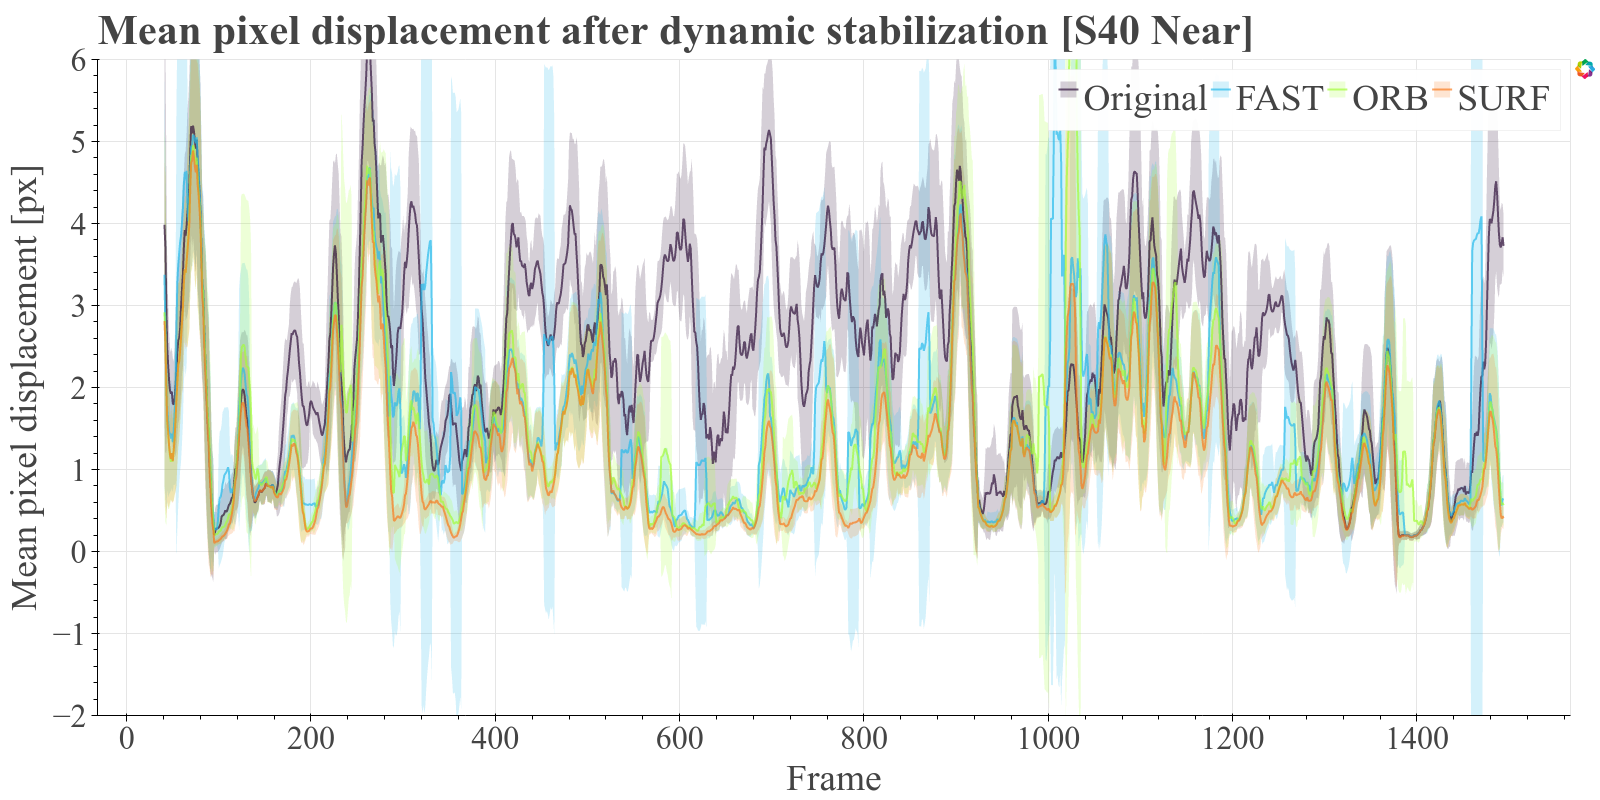
\includegraphics[width=0.475\linewidth]{diagrams/optical_flow/s40_n_near_image_raw.mp4.csv/compare_of_mean_pixel_displacement/window_size_12.html.png}    & 
      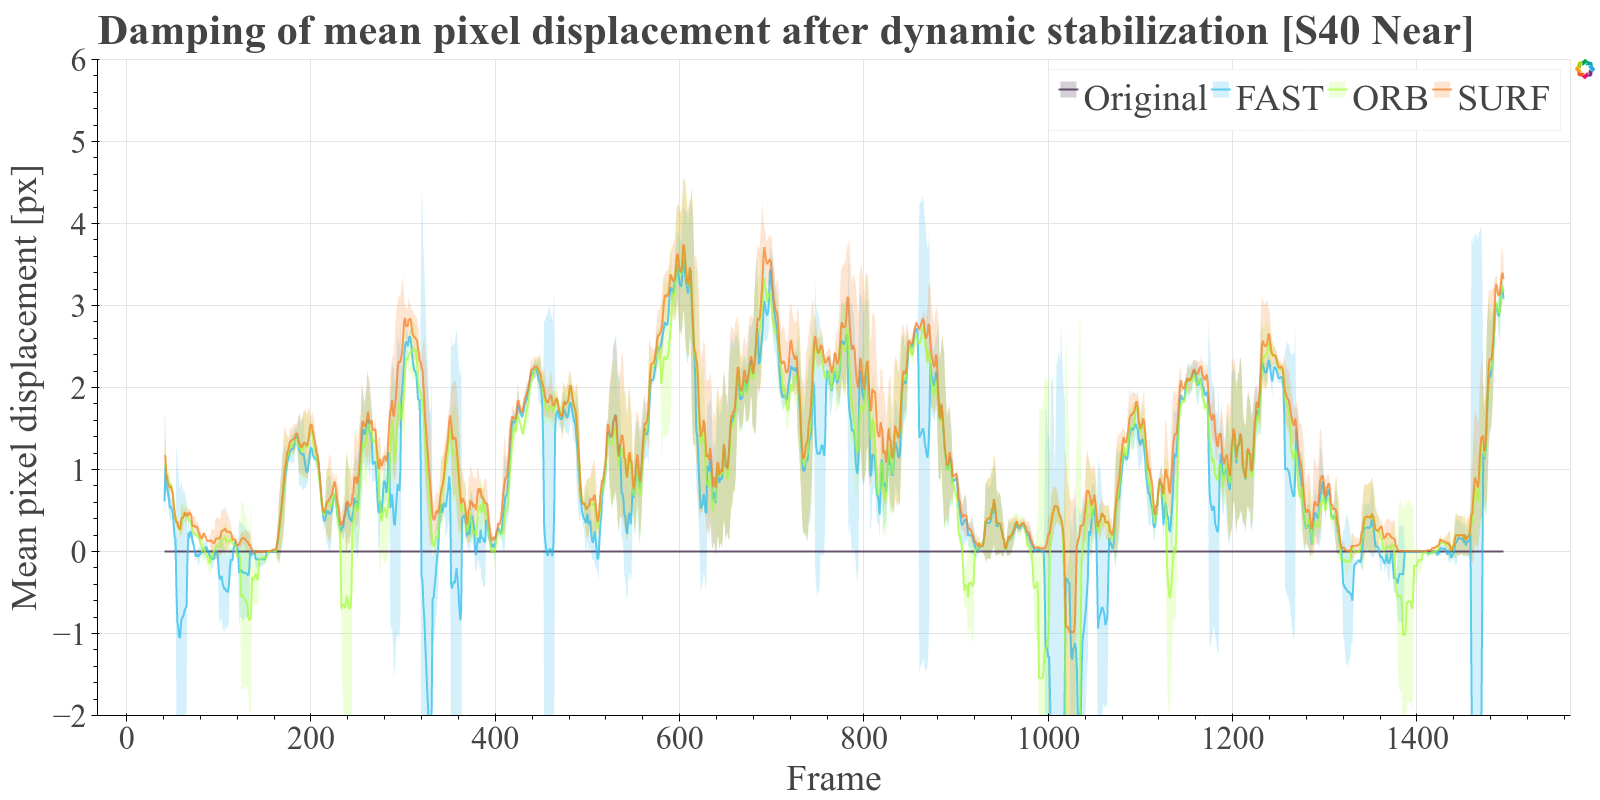
\includegraphics[width=0.475\linewidth]{diagrams/optical_flow/s40_n_near_image_raw.mp4.csv/deltas_of_mean_pixel_displacement/window_size_12.html.png}   \\ 

      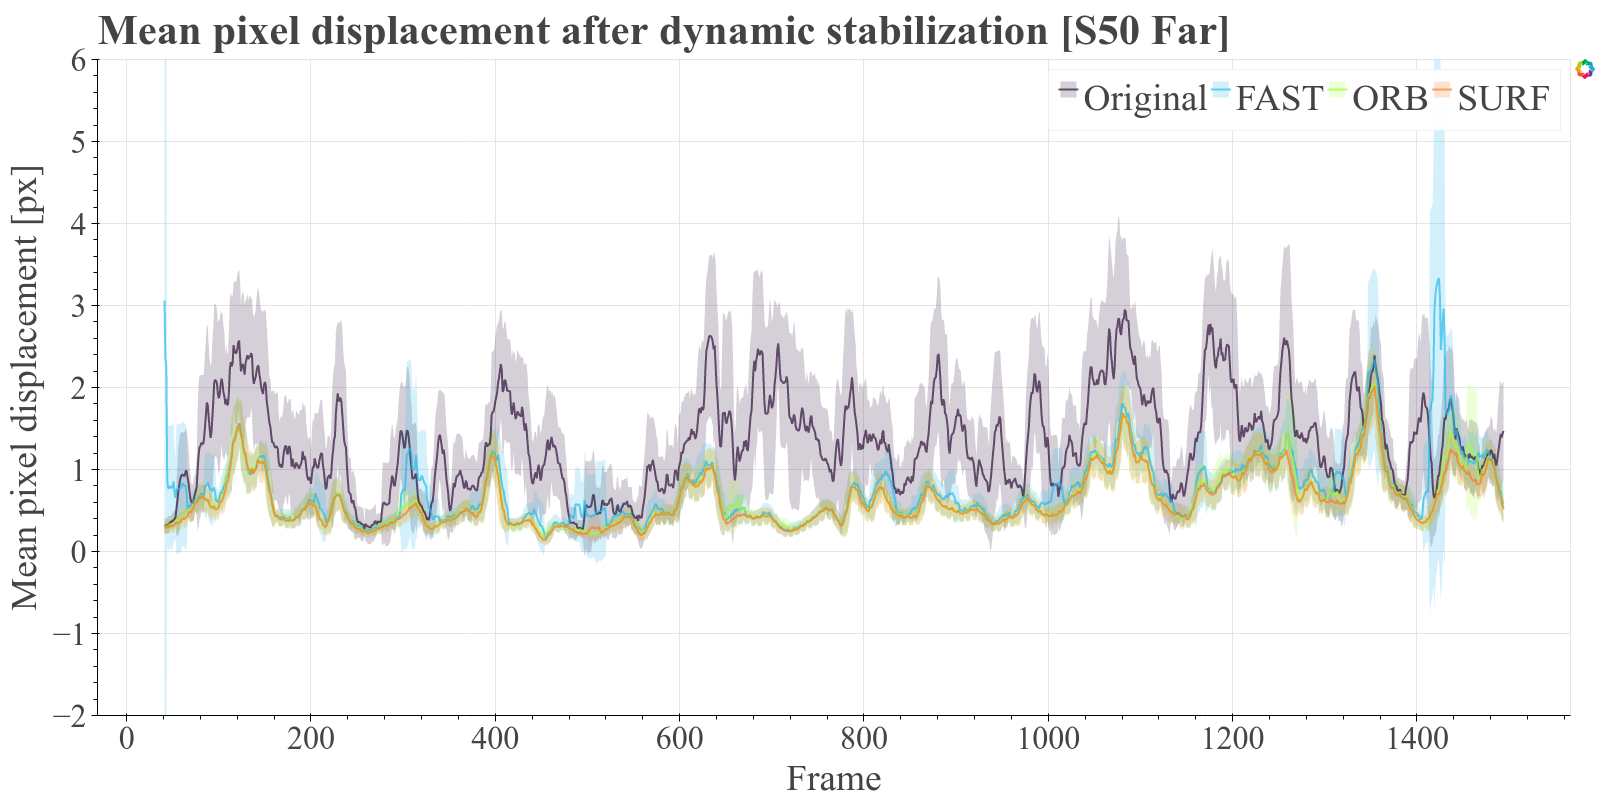
\includegraphics[width=0.475\linewidth]{diagrams/optical_flow/s50_s_far_image_raw.mp4.csv/compare_of_mean_pixel_displacement/window_size_12.html.png}    & 
      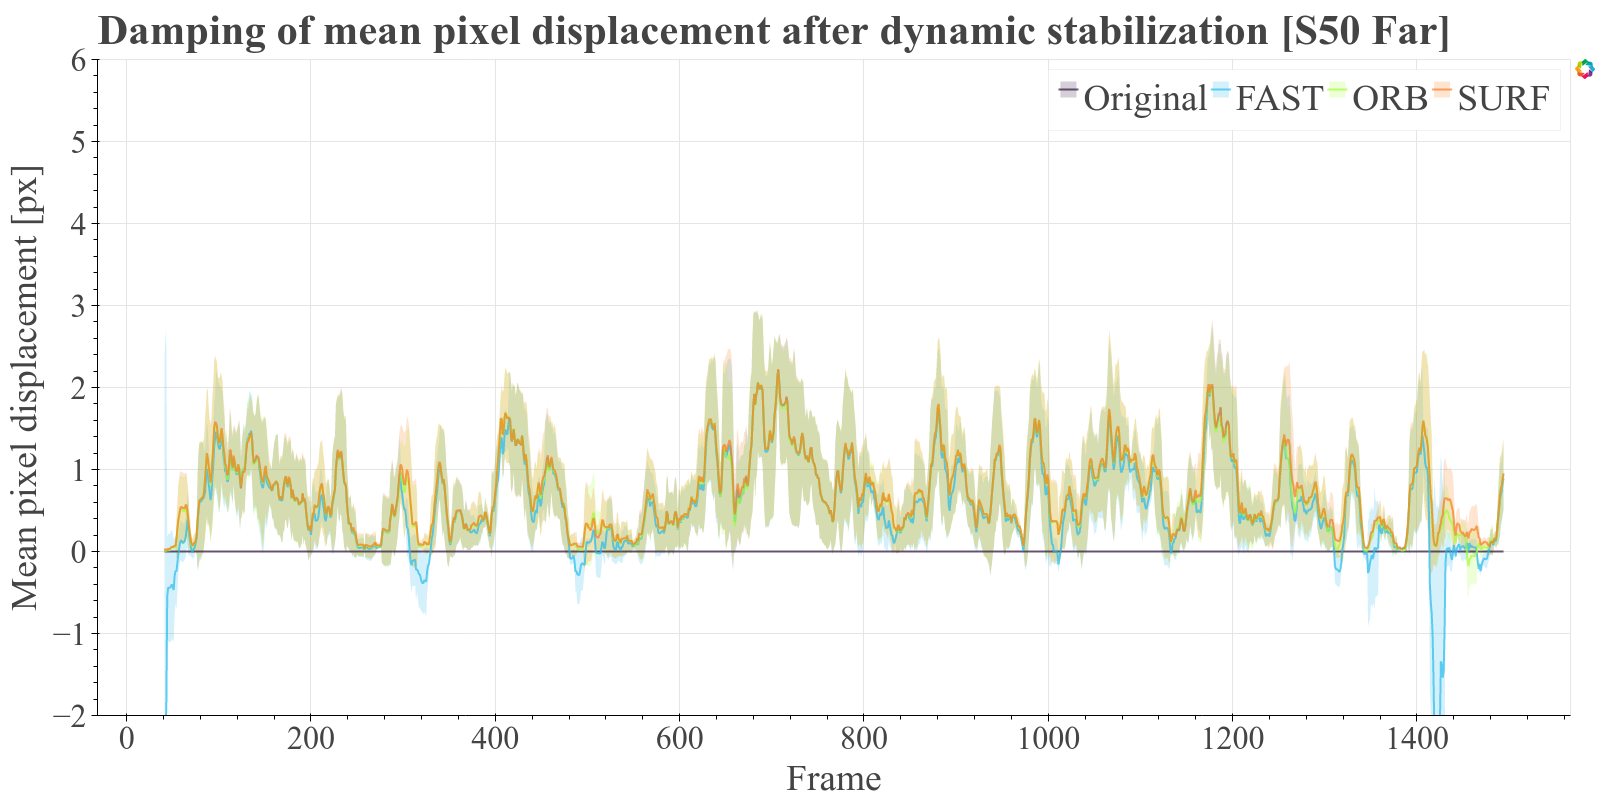
\includegraphics[width=0.475\linewidth]{diagrams/optical_flow/s50_s_far_image_raw.mp4.csv/deltas_of_mean_pixel_displacement/window_size_12.html.png}   \\ 

      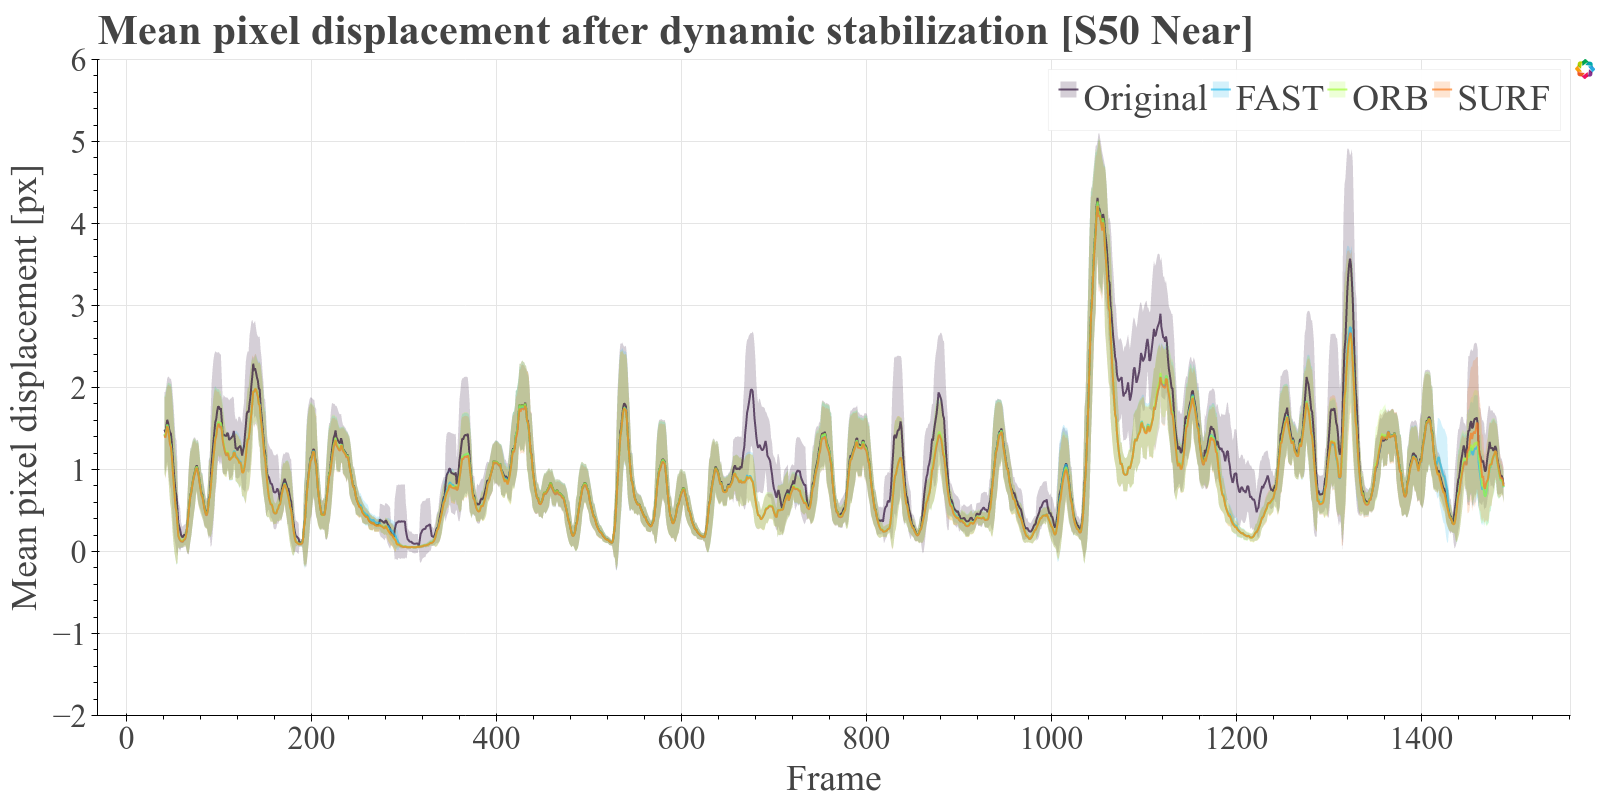
\includegraphics[width=0.475\linewidth]{diagrams/optical_flow/s50_s_near_image_raw.mp4.csv/compare_of_mean_pixel_displacement/window_size_12.html.png}    &   
      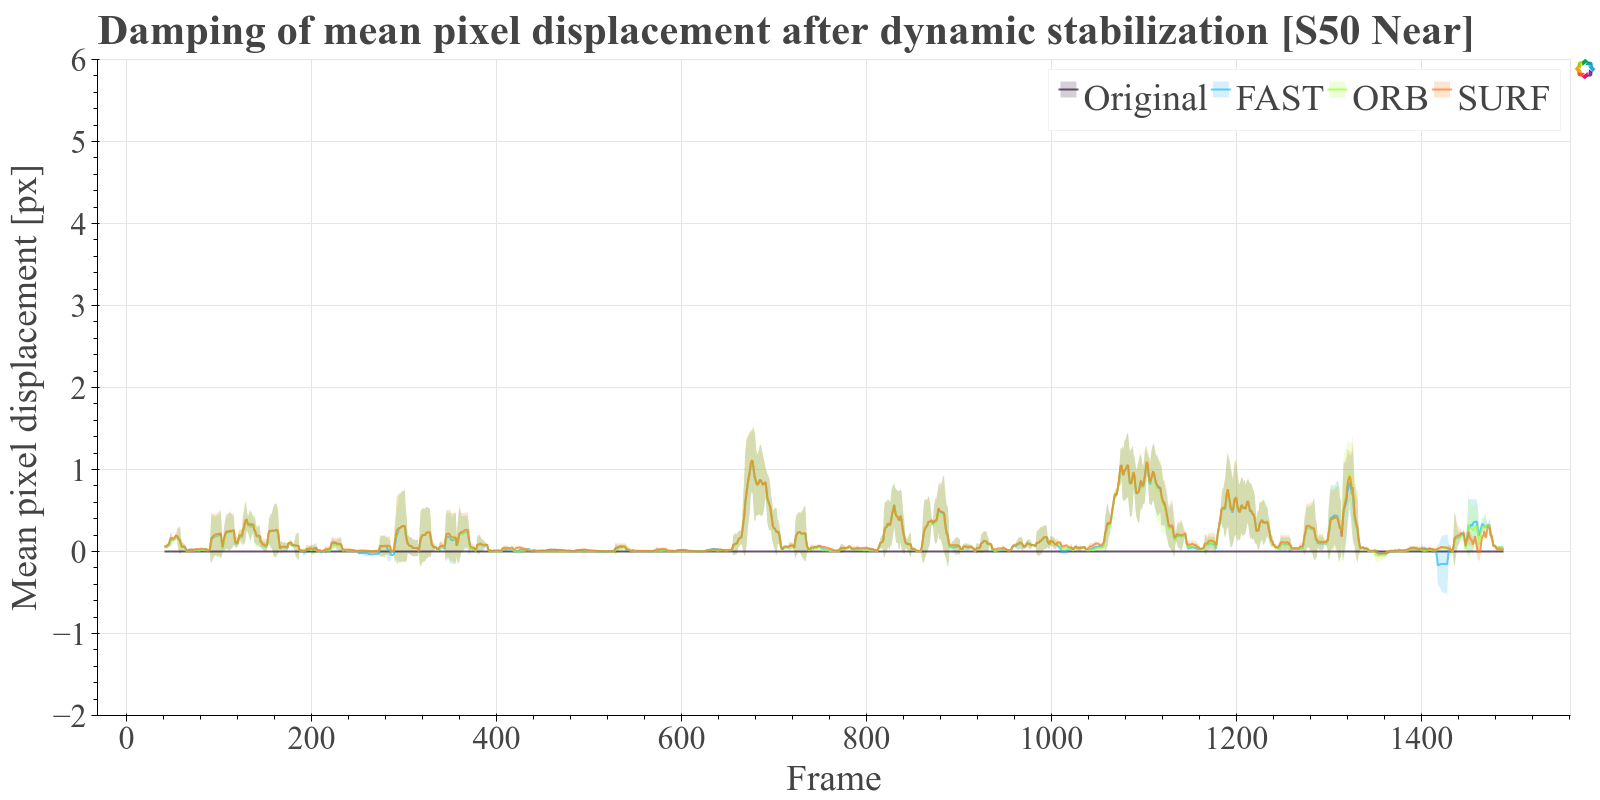
\includegraphics[width=0.475\linewidth]{diagrams/optical_flow/s50_s_near_image_raw.mp4.csv/deltas_of_mean_pixel_displacement/window_size_12.html.png}   \\ 
    \end{tabular}
    \caption{
        Left: 
        The mean pixel shifts after stabilization with SURF, ORB and FAST compared to the original not stabilized video feed using optical flow as measure (lower is better).
        Right: 
        The damping of the mean pixel shifts of the same three stabilizers (higher is better). 
        The graphs approximate the removed jitter in the mean pixel shift between the original video and the stabilizers at each frame.\\
        For visualization the values are filtered using the rolling mean over 12 frames. 
        The light areas display the standard deviation within the window. \\
        It shows that for each of the stabilizers the damping is substantial, removes most of the jitter introduced by environmental influences and leaves only wanted movement of vehicles in the dynamic foreground.
    }
    \label{fig:dynamic_stabilization_appendix}
    \end{figure*}

    


\begin{figure*}[!ht]
  \centering
  \begin{tabular}{cc}
    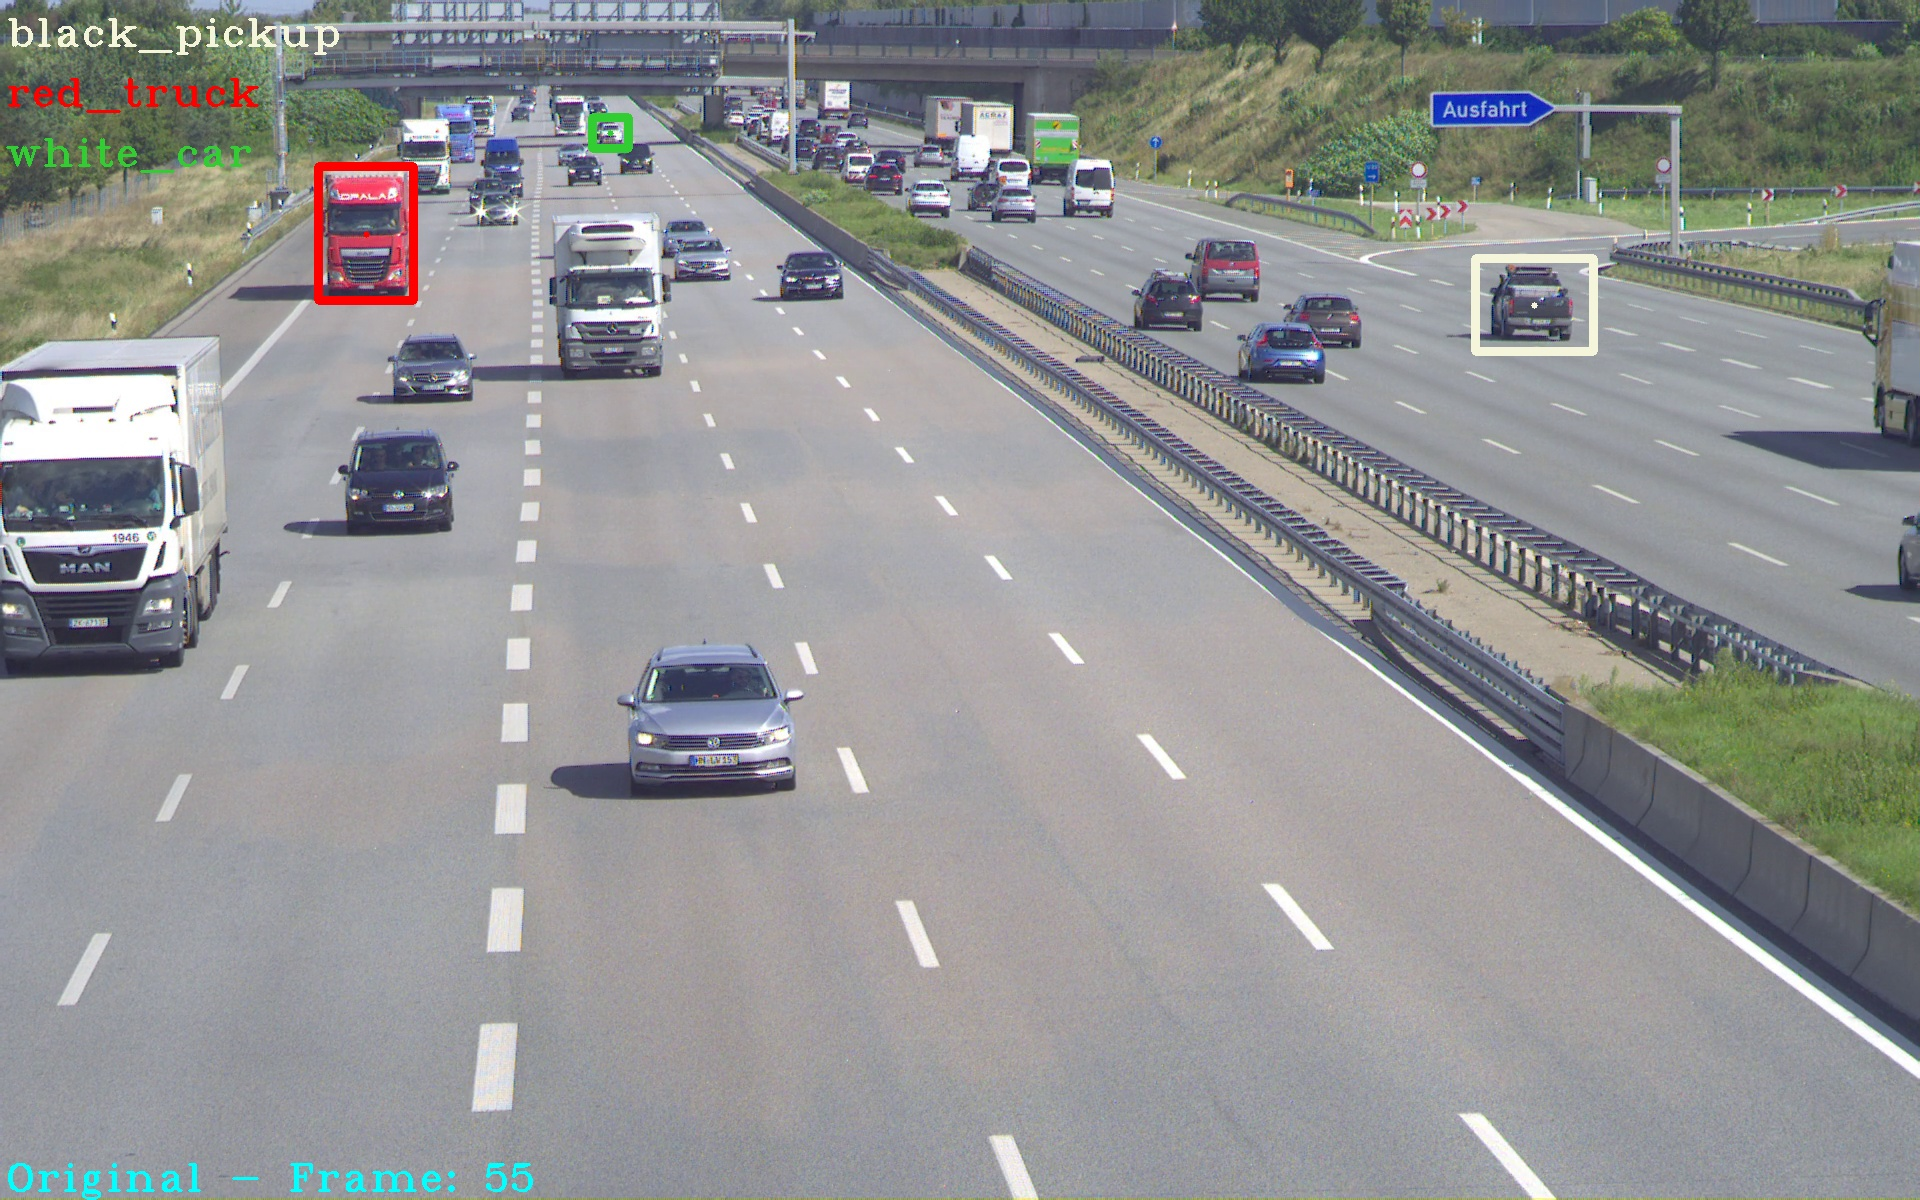
\includegraphics[width=0.45\linewidth]{diagrams/object_tracking/s40_n_far/frame.png}    &  
    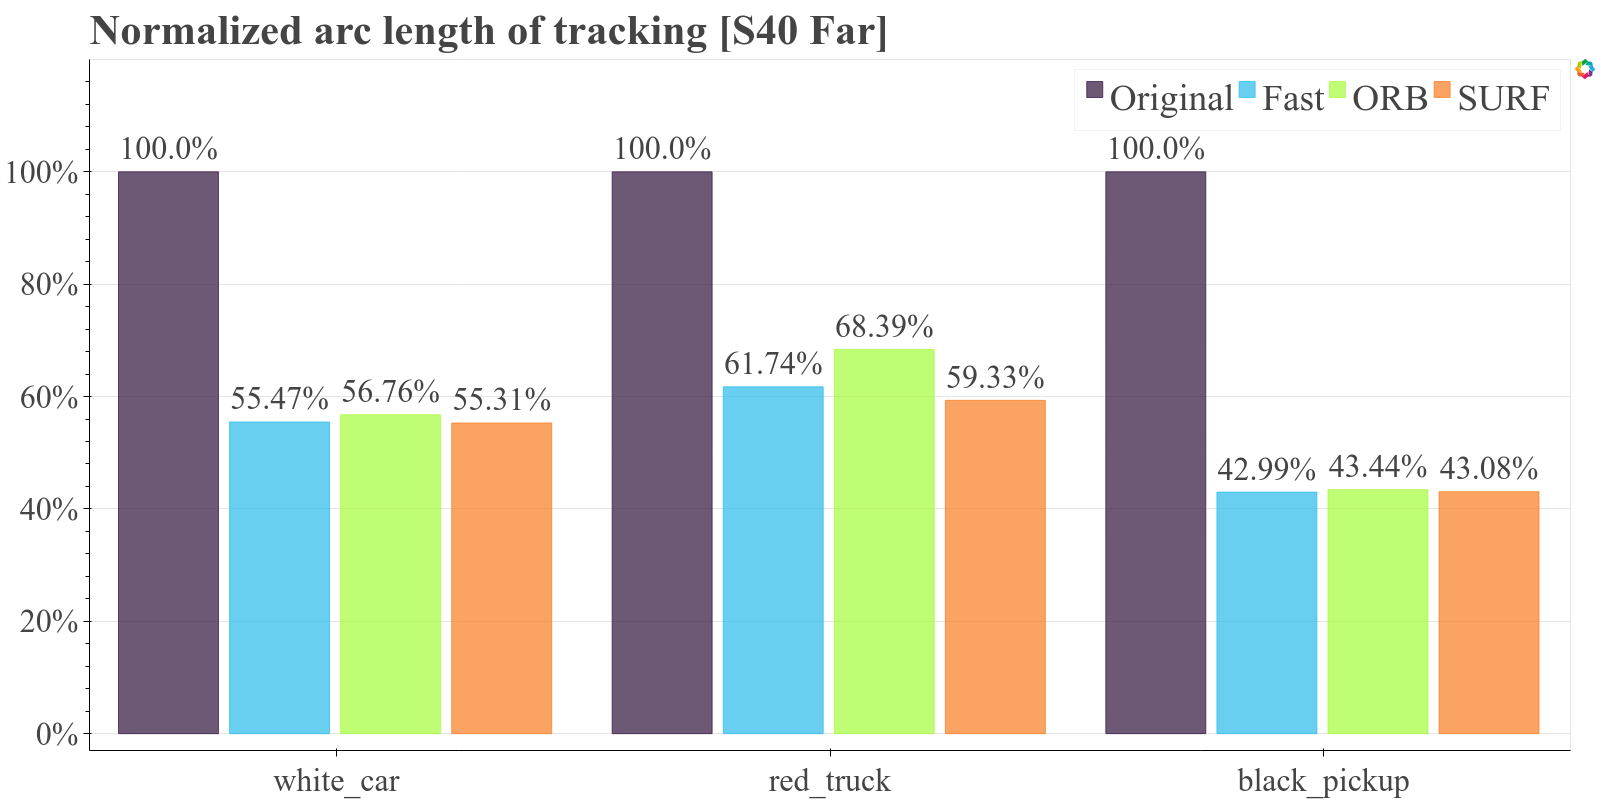
\includegraphics[width=0.475\linewidth]{diagrams/object_tracking/s40_n_far/normalized_arc_lengths.html.png}    \\

    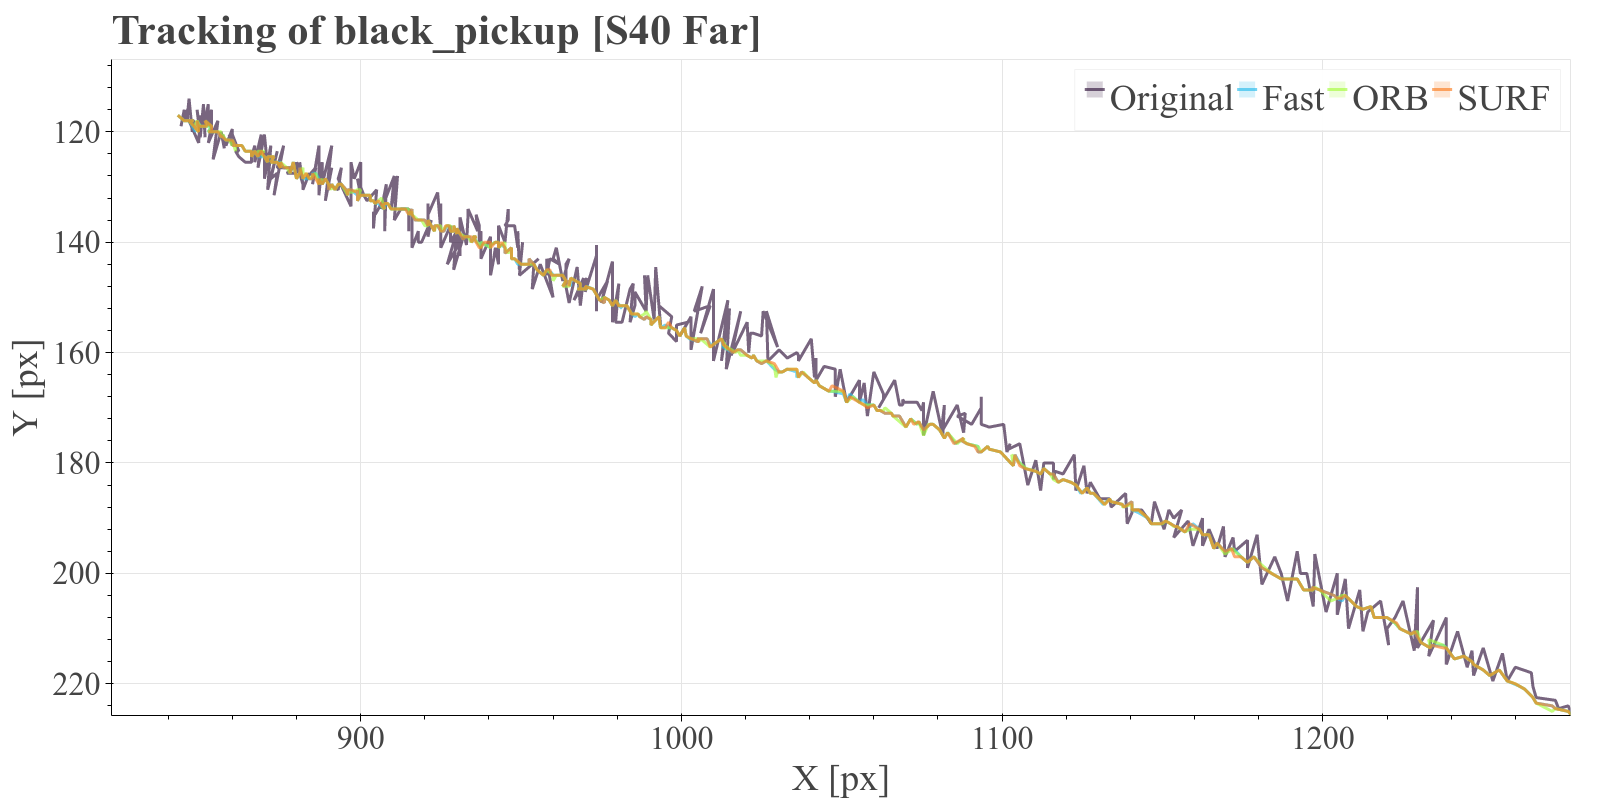
\includegraphics[width=0.475\linewidth]{diagrams/object_tracking/s40_n_far/black_pickup.png}    &  
    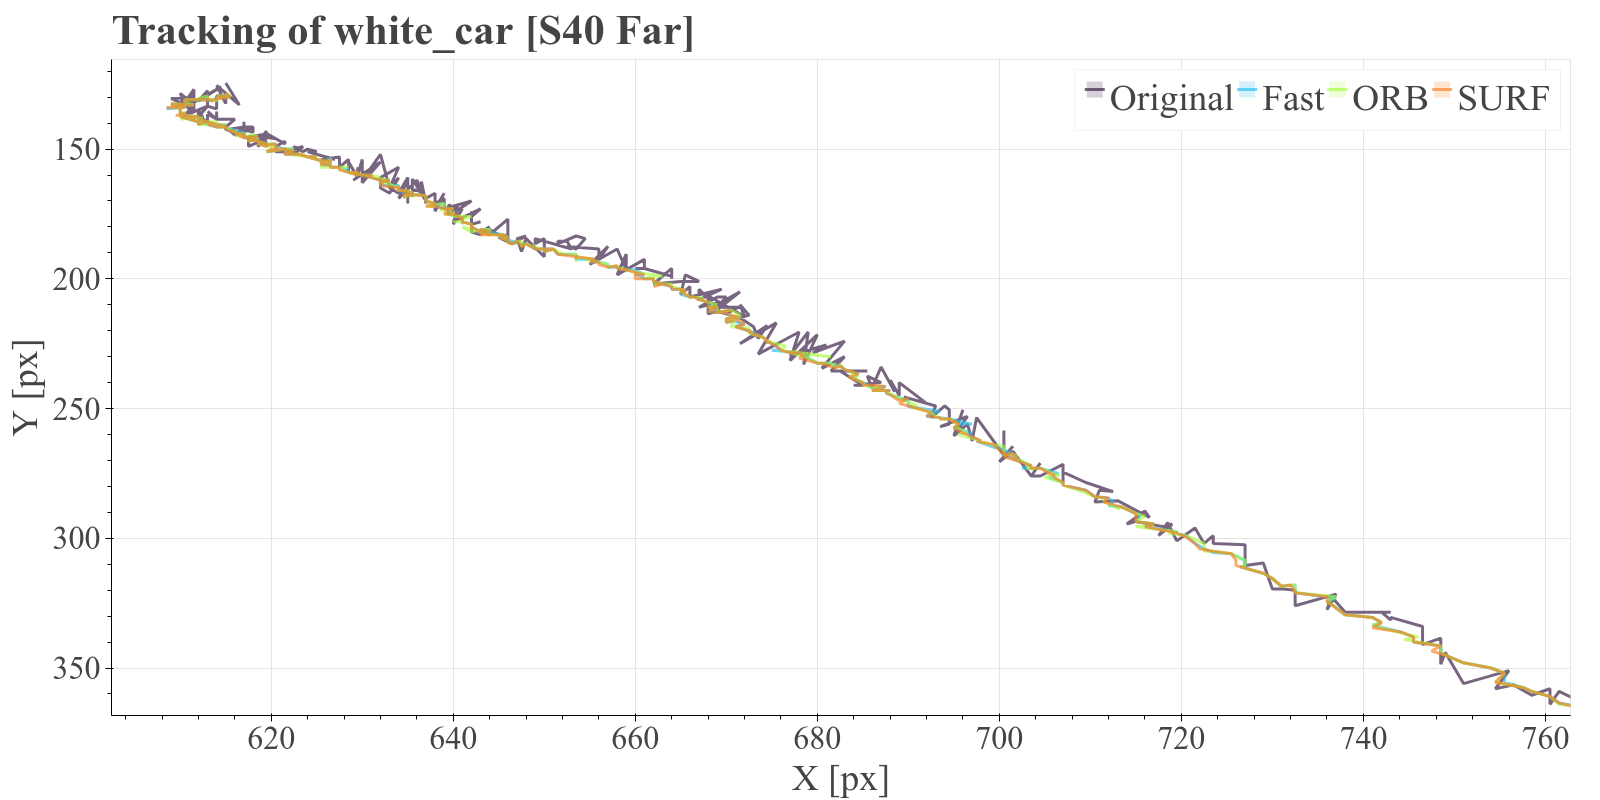
\includegraphics[width=0.475\linewidth]{diagrams/object_tracking/s40_n_far/white_car.png}    \\  
    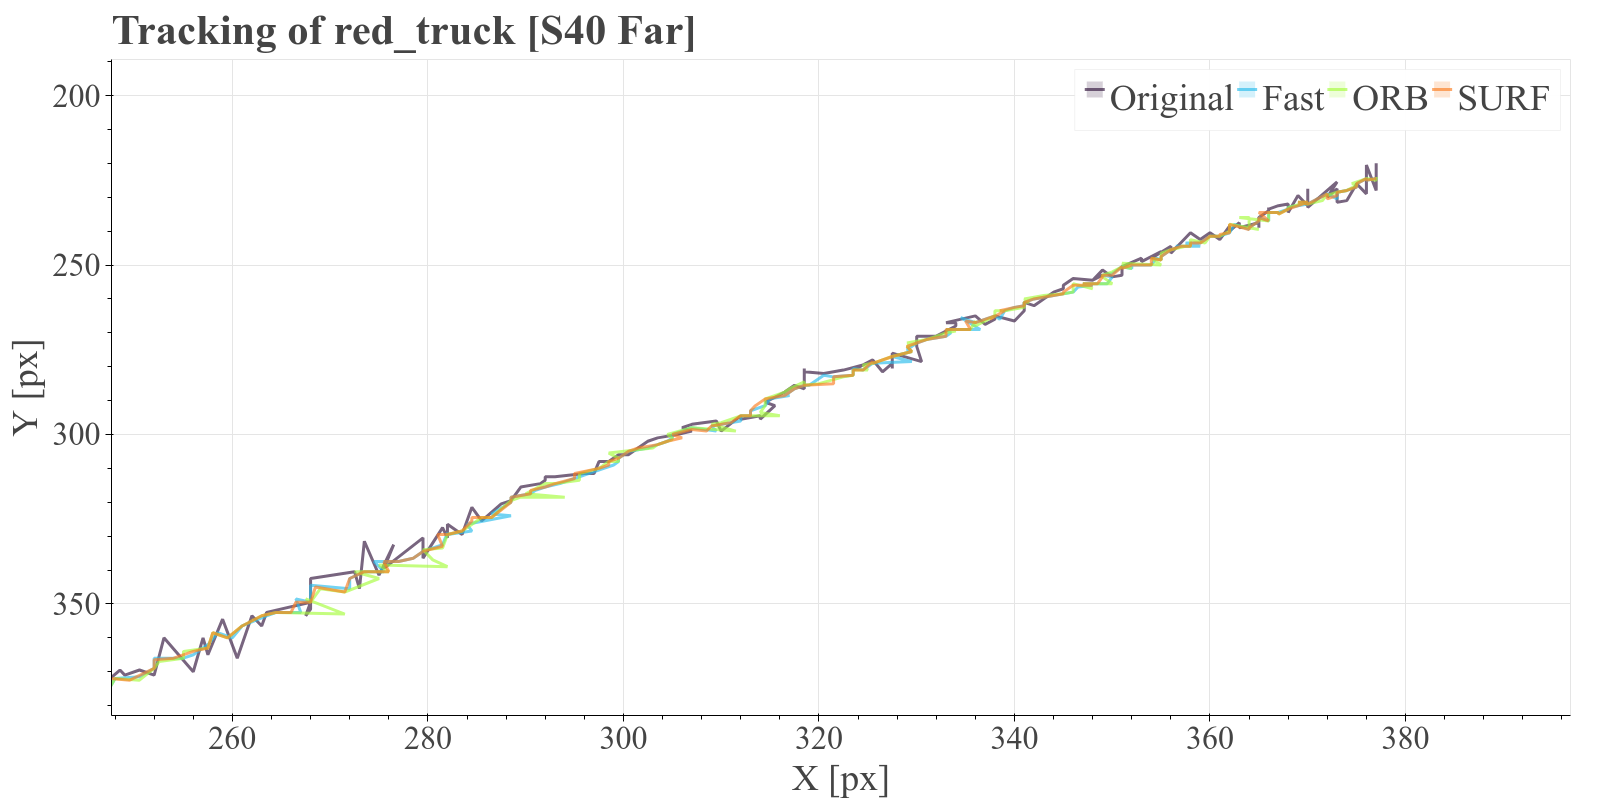
\includegraphics[width=0.475\linewidth]{diagrams/object_tracking/s40_n_far/red_truck.png}   
  \end{tabular}
  \caption{Top Left:
  The tracked vehicles in the camera \camsf{4} marked by their bounding boxes. 
  Top right: 
  The normalized arc lengths representing the path of the tracked pixels through the image.
  Bottom graphs:
  The tracked pixel locations of the vehicles as they move through the scene for the original video feed and the stabilized ones.
  The jittery motion of the camera can be clearly seen by the chaotic movement of the pixels.
  After stabilization the pixels move much more smoothly through the images, whereas the remaining jitter is mostly due to inaccuracies in the tracking. 
  }
  \label{fig:object_tracking_appendix_s40_n_far}
\end{figure*}



\begin{figure*}[!ht]
  \centering
  \begin{tabular}{cc}
    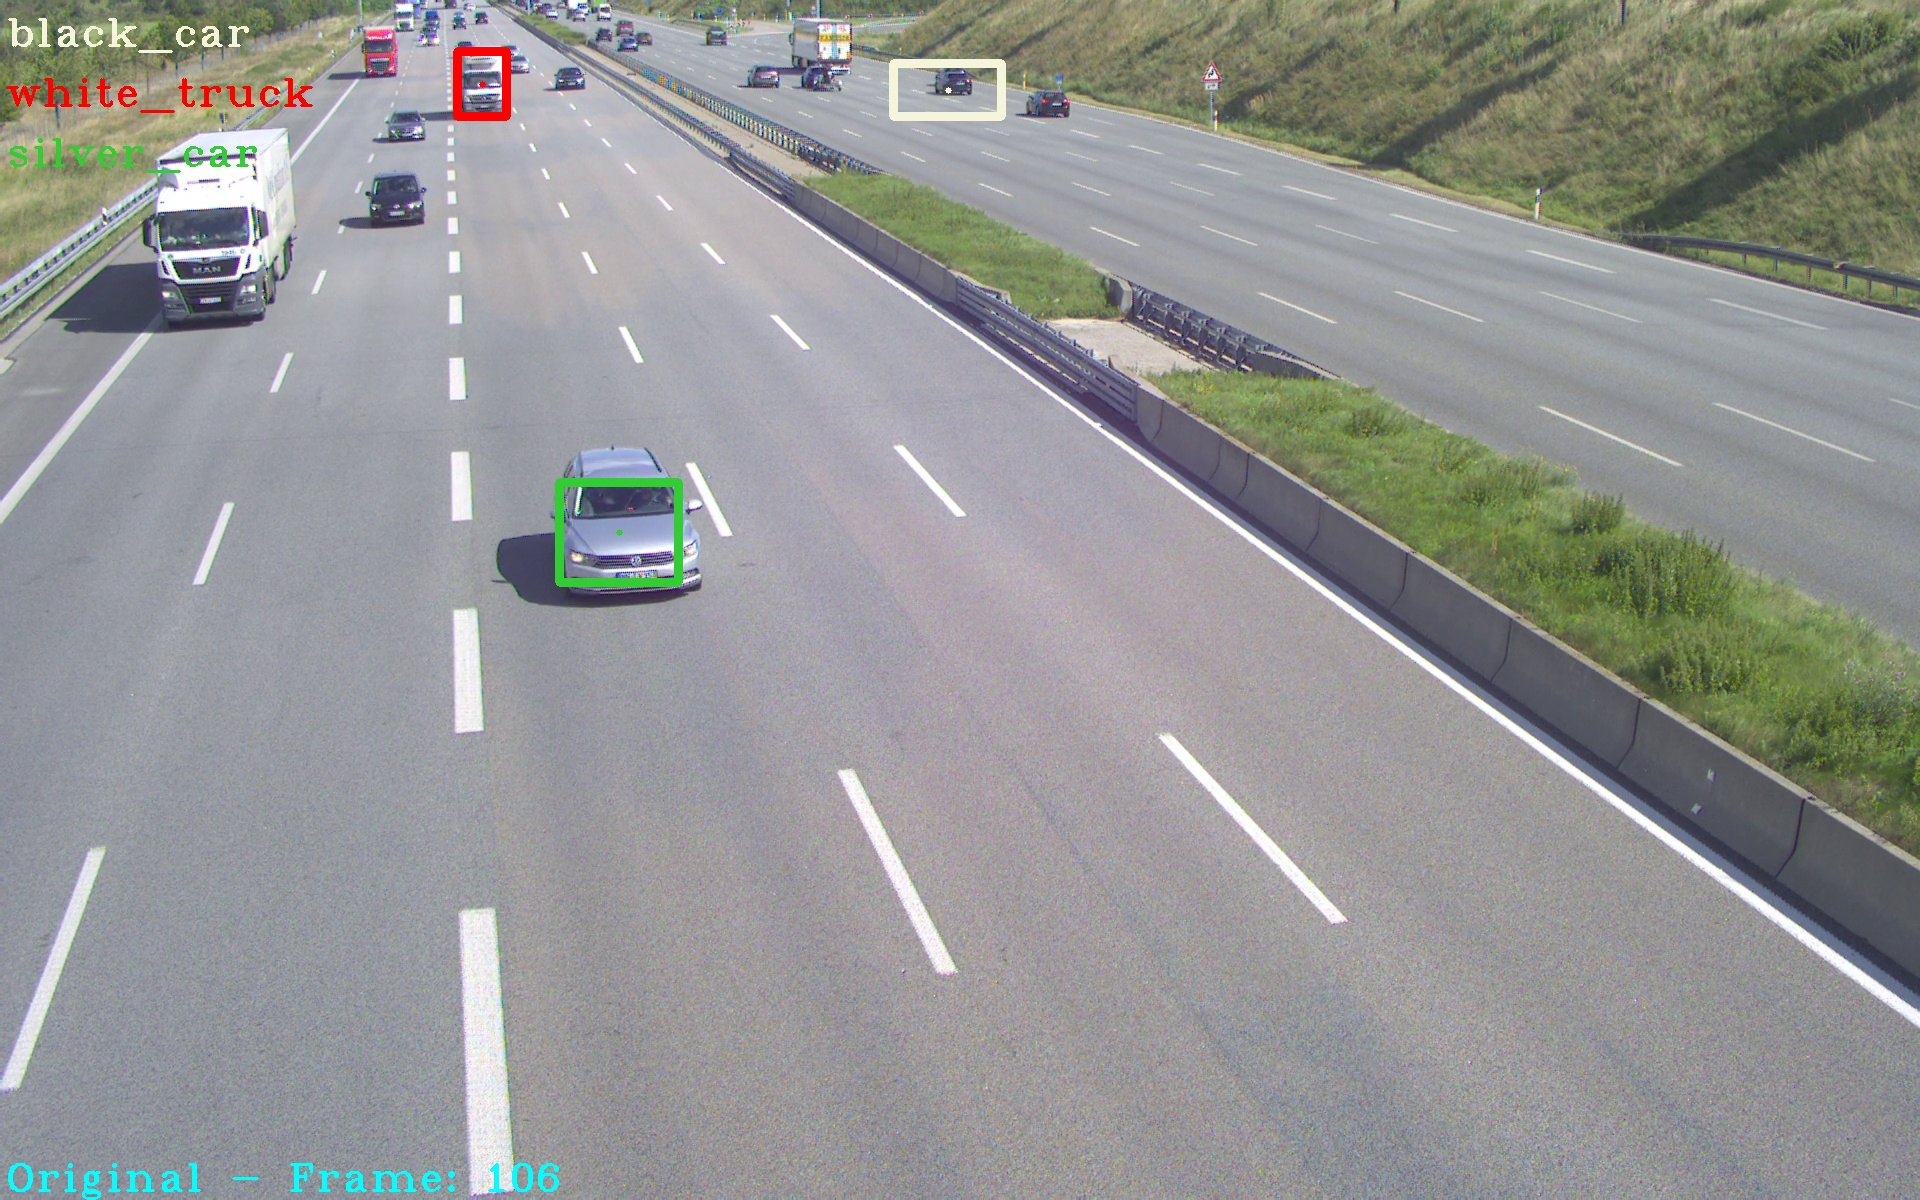
\includegraphics[width=0.45\linewidth]{diagrams/object_tracking/s40_n_near/frame.png}    &  
    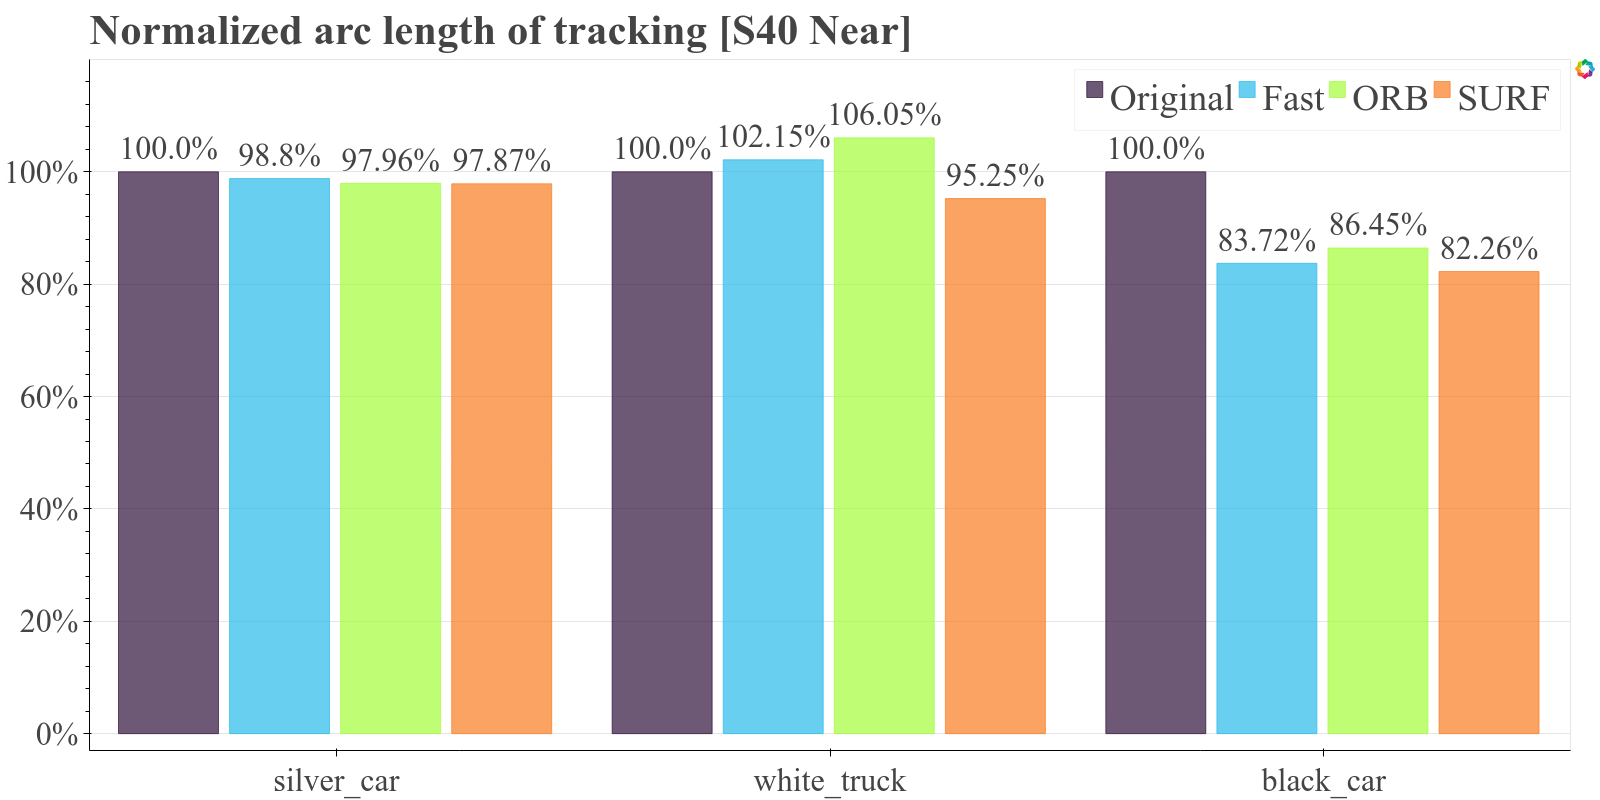
\includegraphics[width=0.475\linewidth]{diagrams/object_tracking/s40_n_near/normalized_arc_lengths.html.png}    \\

    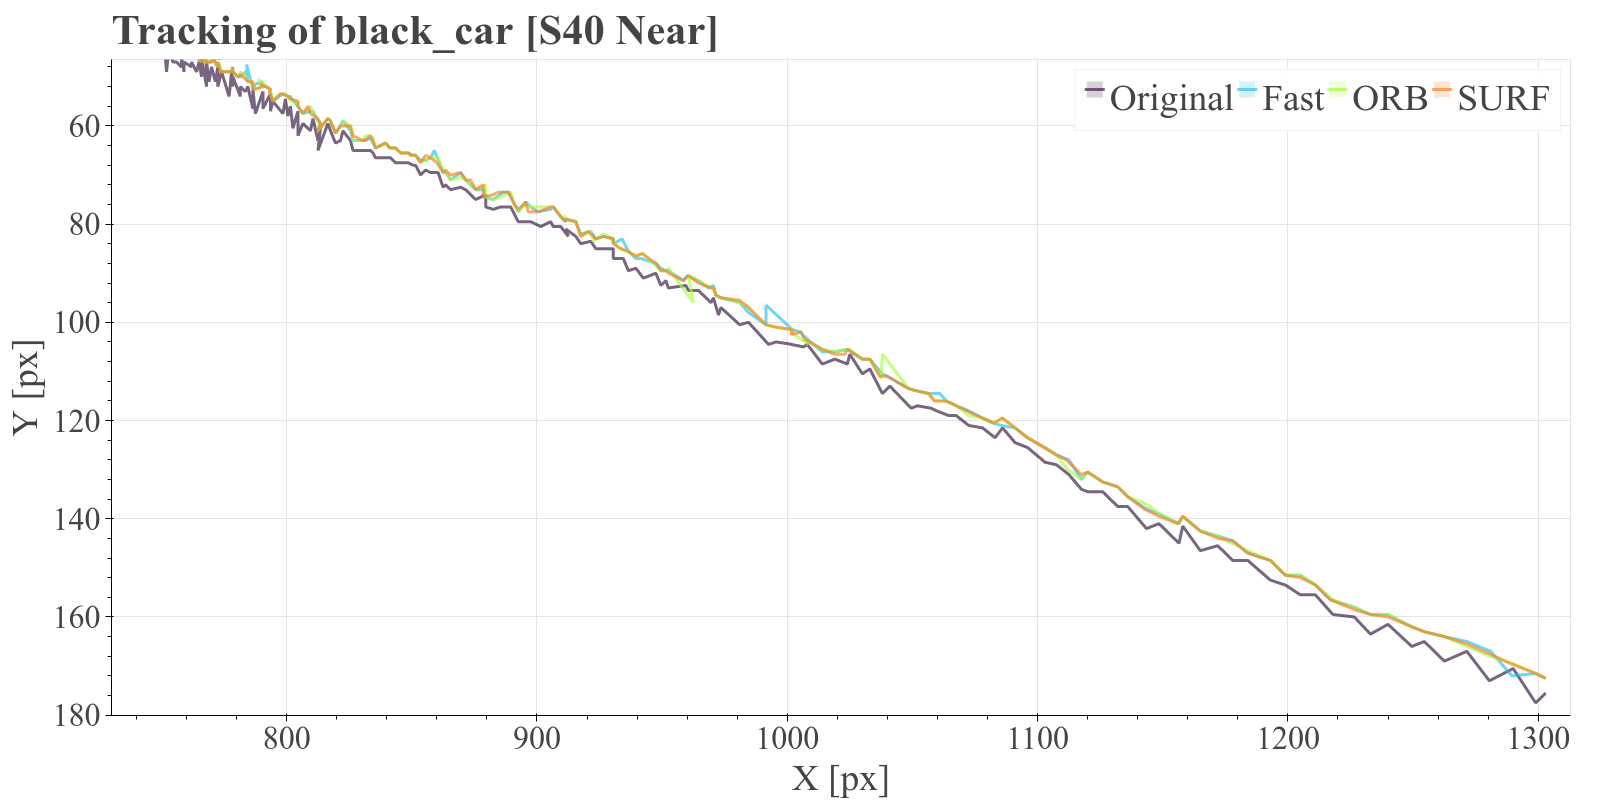
\includegraphics[width=0.475\linewidth]{diagrams/object_tracking/s40_n_near/black_car.png}    &  
    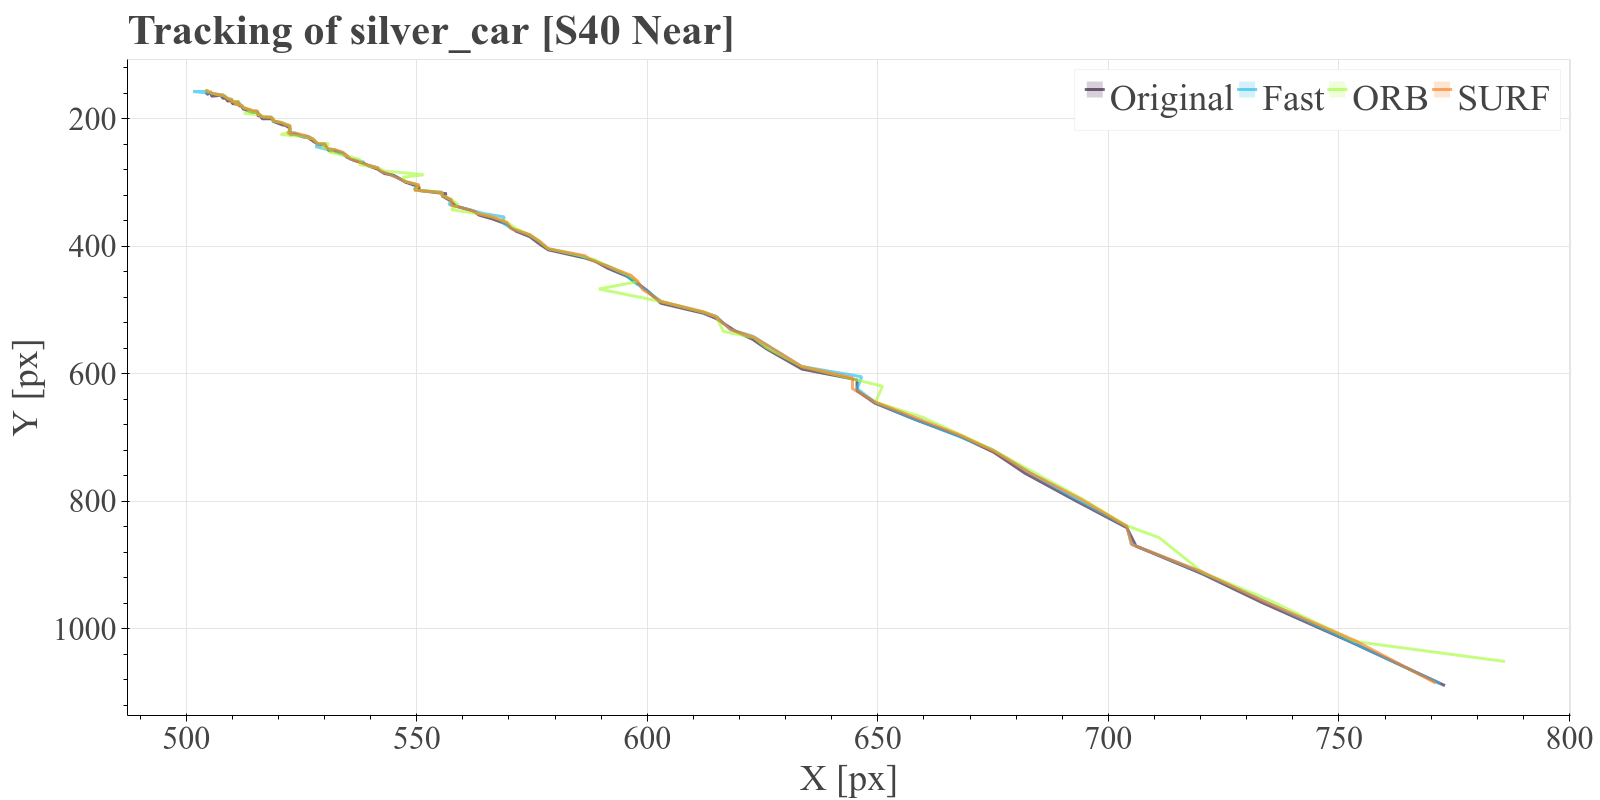
\includegraphics[width=0.475\linewidth]{diagrams/object_tracking/s40_n_near/silver_car.png}    \\  
    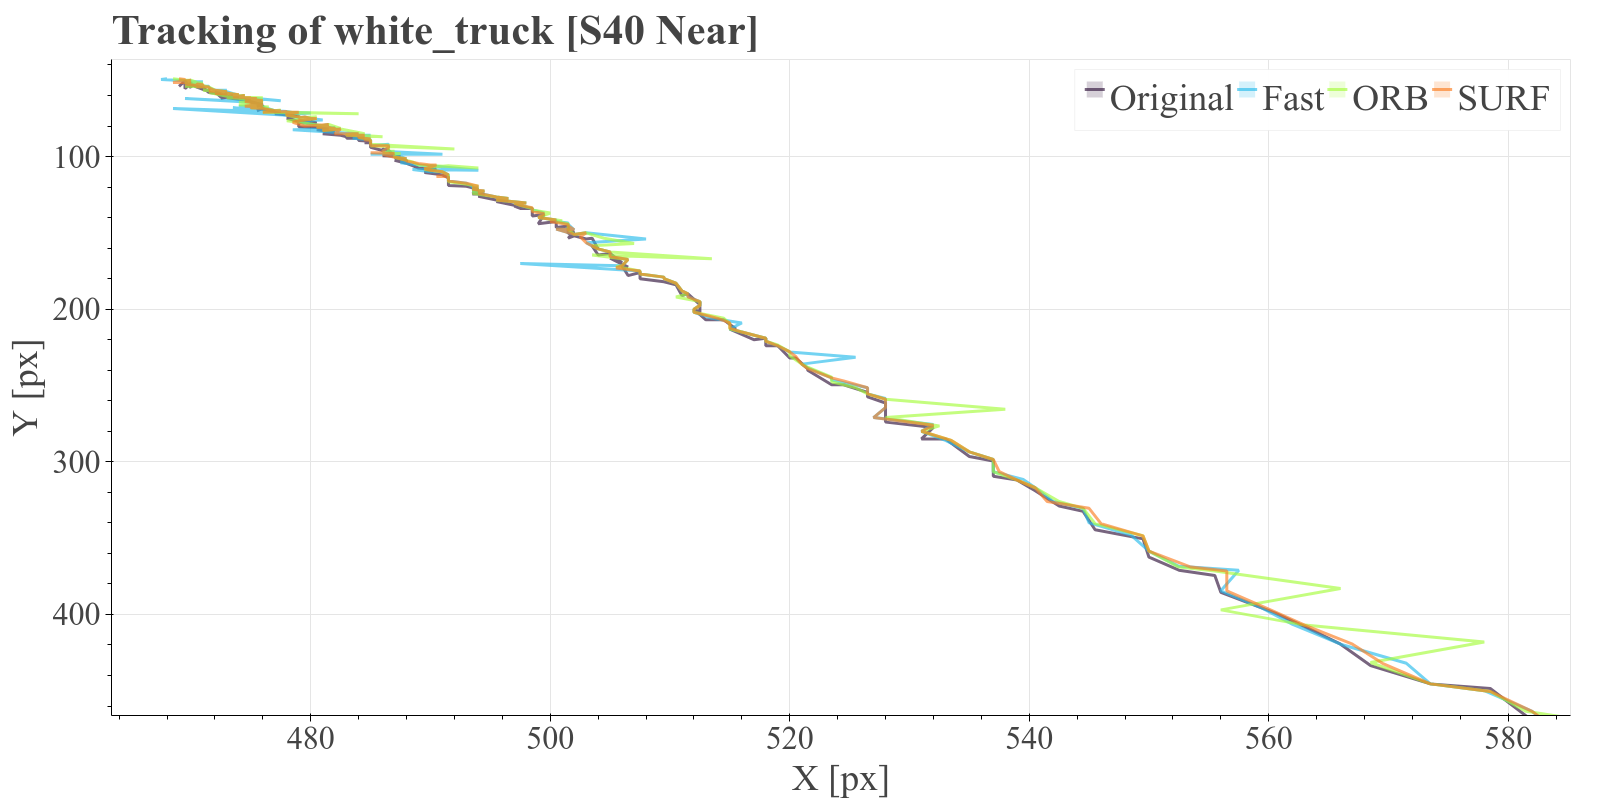
\includegraphics[width=0.475\linewidth]{diagrams/object_tracking/s40_n_near/white_truck.png}   
  \end{tabular}
  \caption{Top Left:
  The tracked vehicles in the camera \camsn{4} marked by their bounding boxes. 
  Top right: 
  The normalized arc lengths representing the path of the tracked pixels through the image.
  Bottom graphs:
  The tracked pixel locations of the vehicles as they move through the scene for the original video feed and the stabilized ones.
  It shows that the recording did not include much jitter and thus the paths are already relatively smooth.
   }
  \label{fig:object_tracking_appendix_s40_n_near}
\end{figure*}



\begin{figure*}[!ht]
  \centering
  \begin{tabular}{cc}
    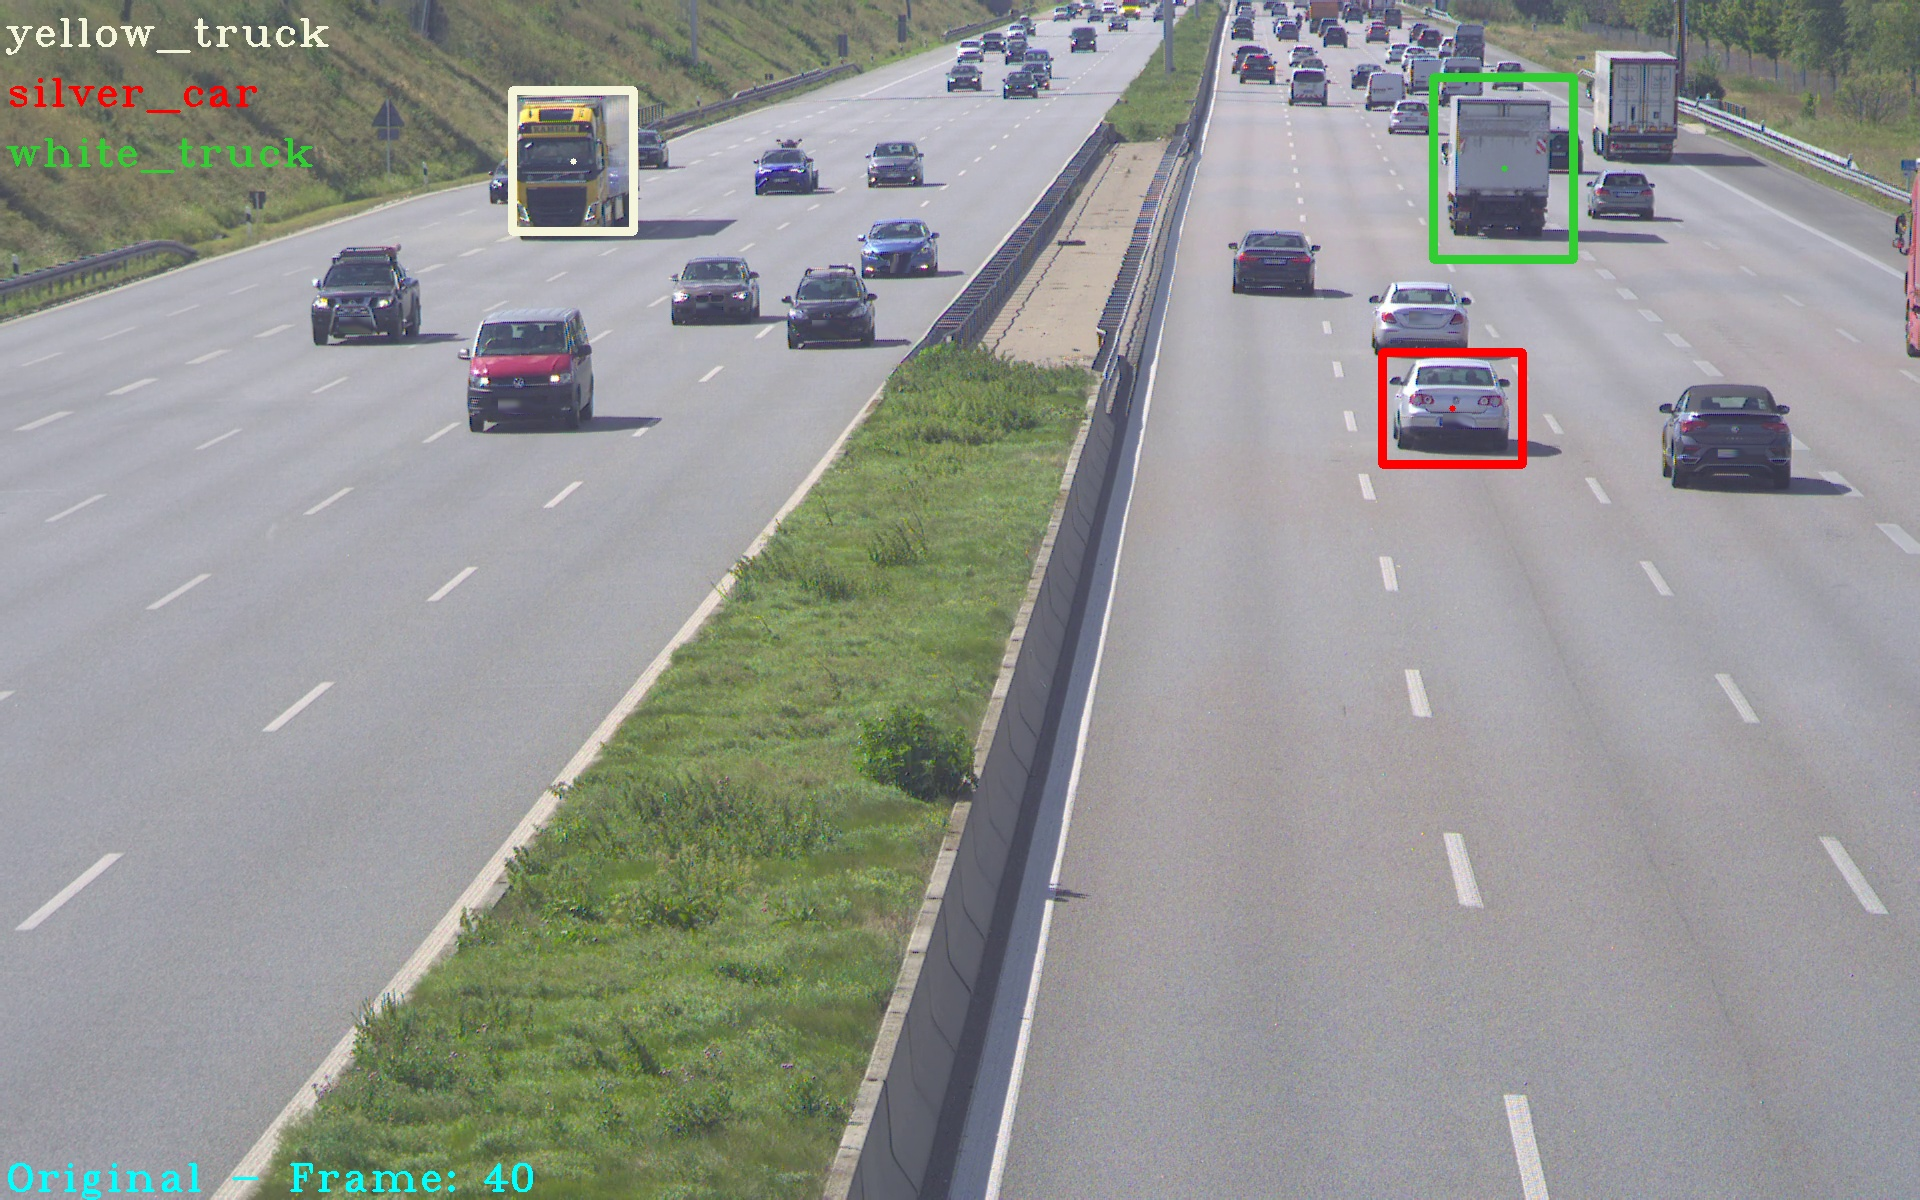
\includegraphics[width=0.45\linewidth]{diagrams/object_tracking/s50_s_far/frame.png}    &  
    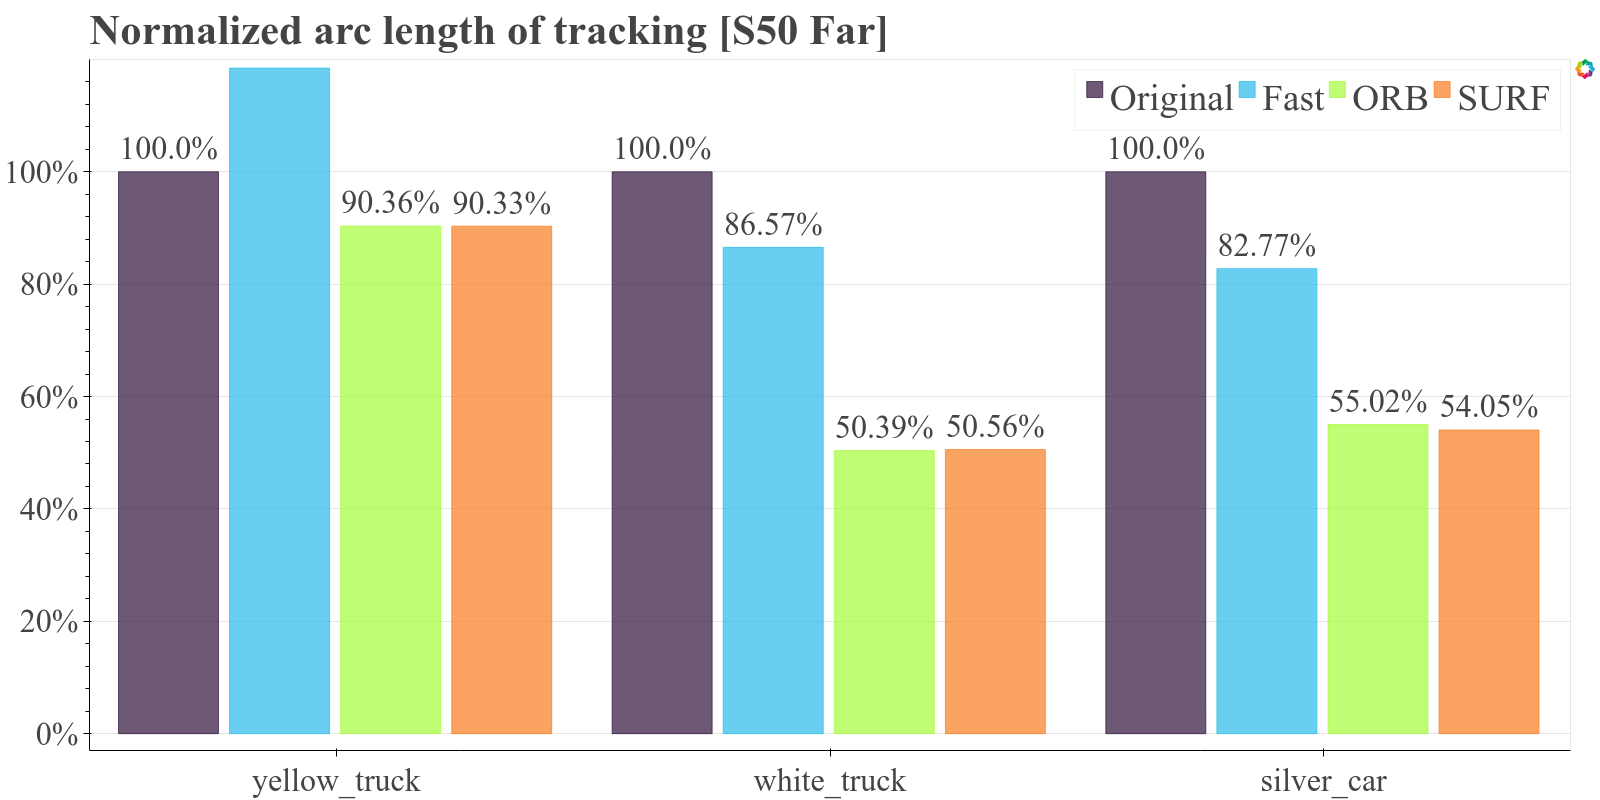
\includegraphics[width=0.475\linewidth]{diagrams/object_tracking/s50_s_far/normalized_arc_lengths.html.png}    \\

    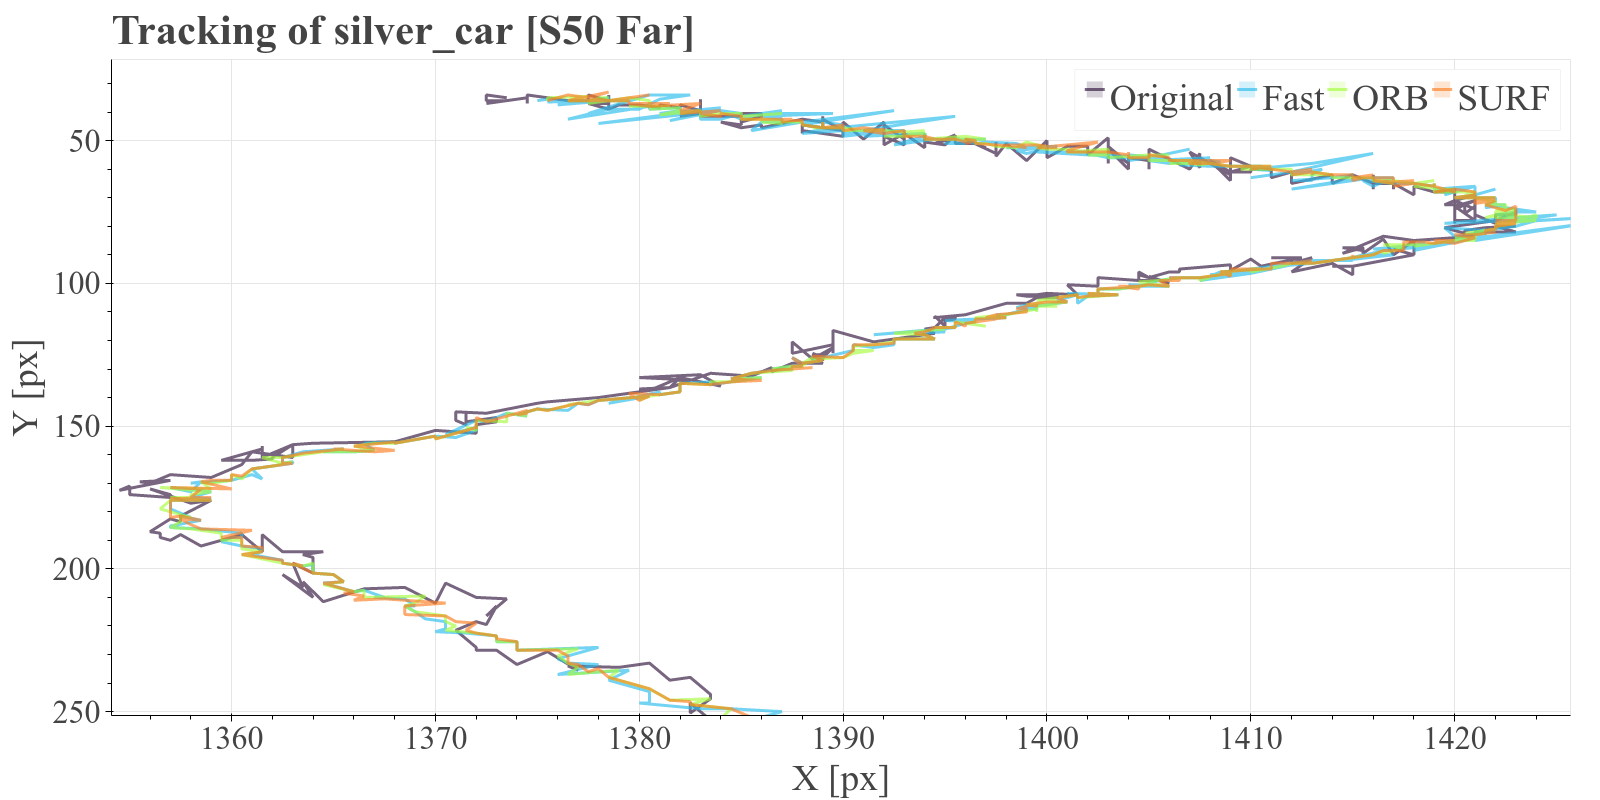
\includegraphics[width=0.475\linewidth]{diagrams/object_tracking/s50_s_far/silver_car.png}    &  
    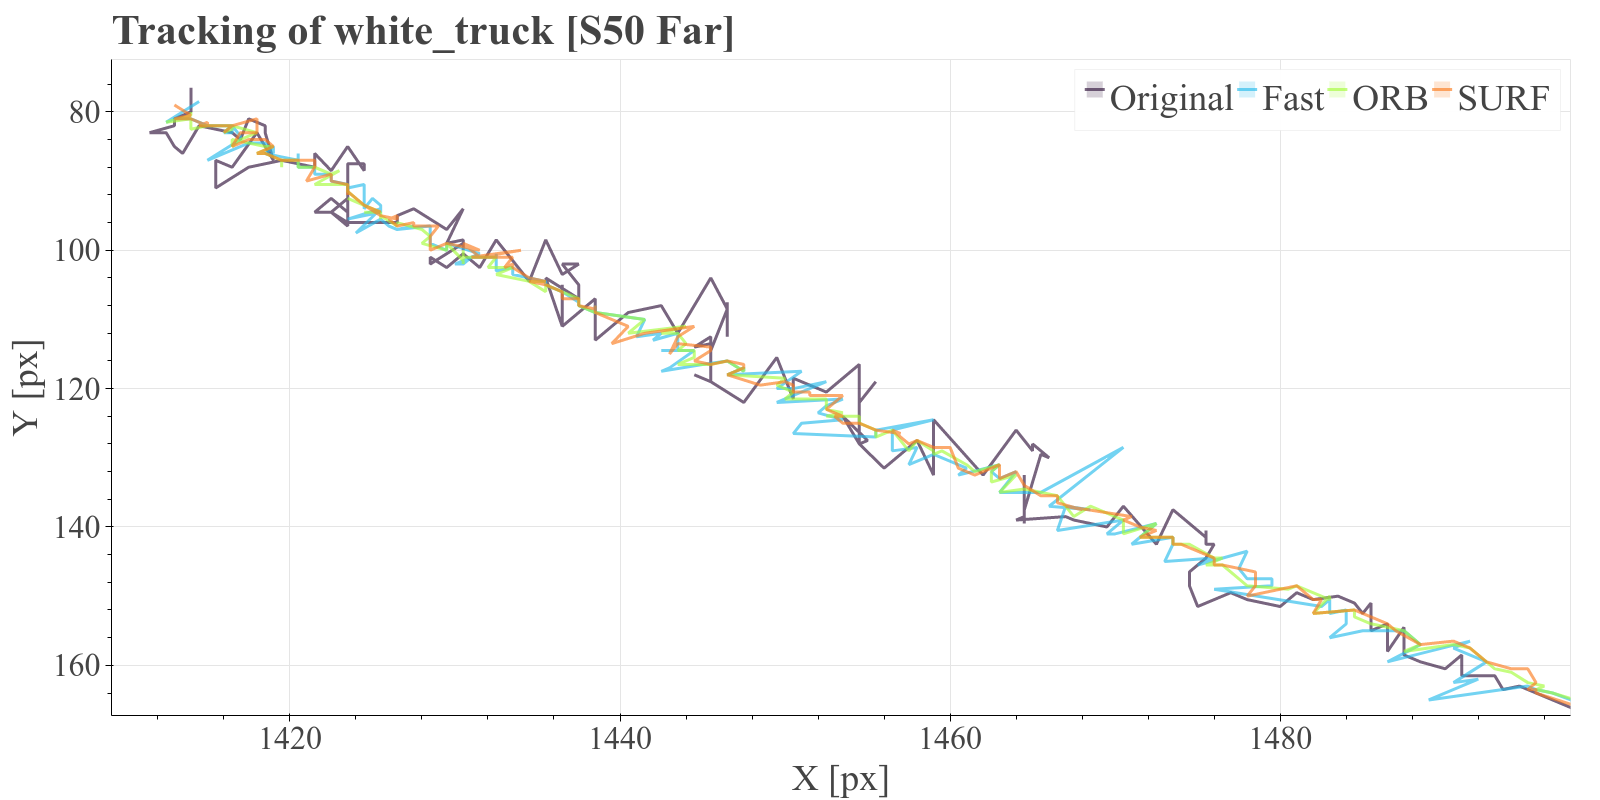
\includegraphics[width=0.475\linewidth]{diagrams/object_tracking/s50_s_far/white_truck.png}    \\  
    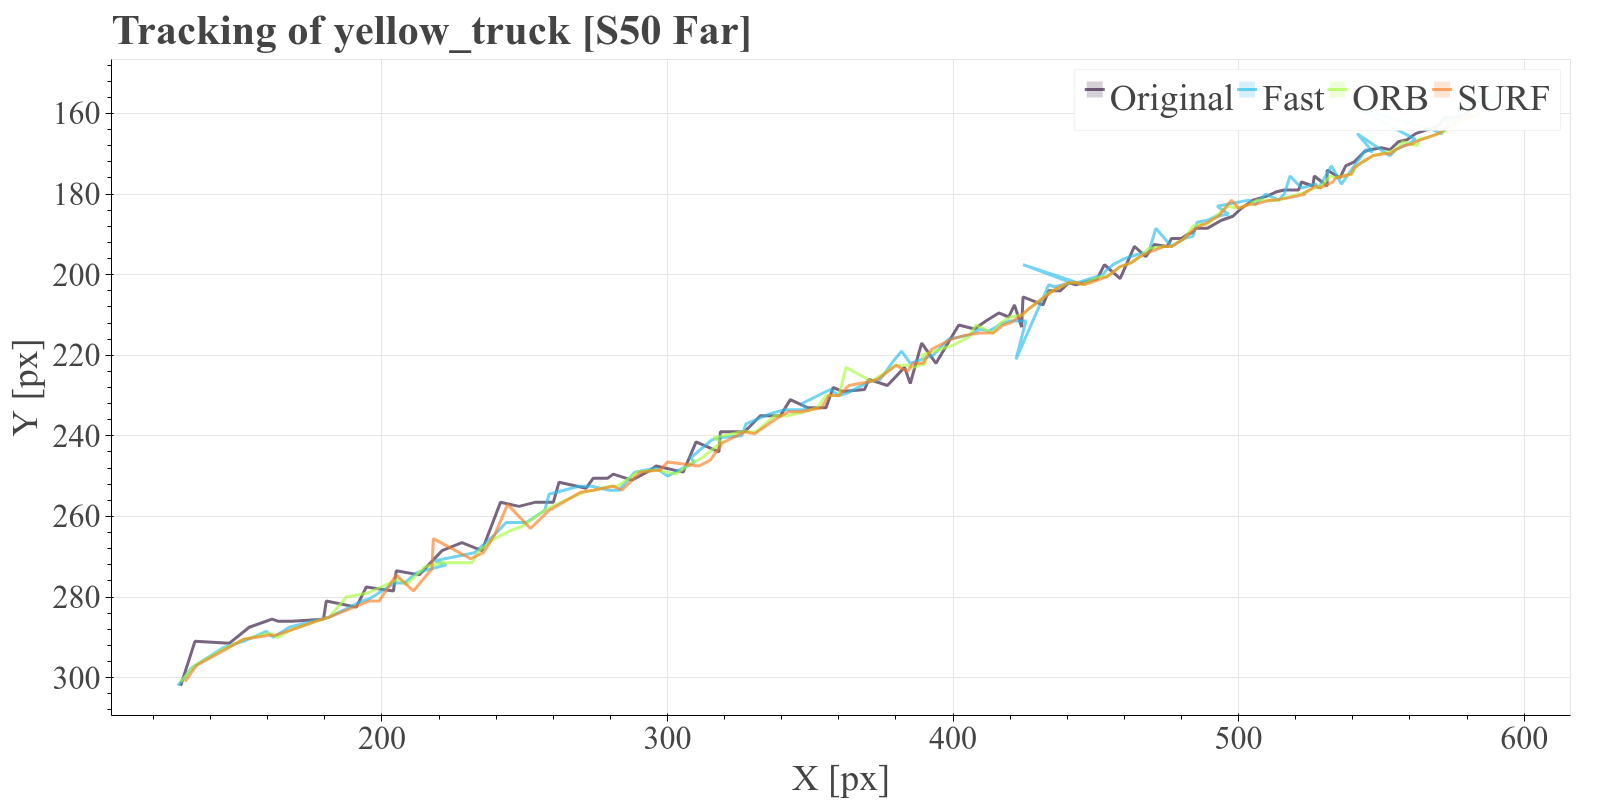
\includegraphics[width=0.475\linewidth]{diagrams/object_tracking/s50_s_far/yellow_truck.png}   
  \end{tabular}
  \caption{Top Left:
  The tracked vehicles in the camera \camsf{5} marked by their bounding boxes. 
  Top right: 
  The normalized arc lengths representing the path of the tracked pixels through the image.
  Bottom graphs:
  The tracked pixel locations of the vehicles as they move through the scene for the original video feed and the stabilized ones.
  The jittery motion of the camera can be clearly seen by the chaotic movement of the pixels.
  After stabilization the pixels move much more smoothly through the images, whereas the remaining jitter is mostly due to inaccuracies in the tracking. 
  The tracking of the silver car displays a lane change of the vehicle over two lanes.
  The tracking of the yellow truck displays an outlier for FAST as it extended the path of the tracked pixel.
  }
  \label{fig:object_tracking_appendix_s50_s_far}
\end{figure*}

\begin{figure*}[!ht]
  \centering
  \begin{tabular}{cc}
    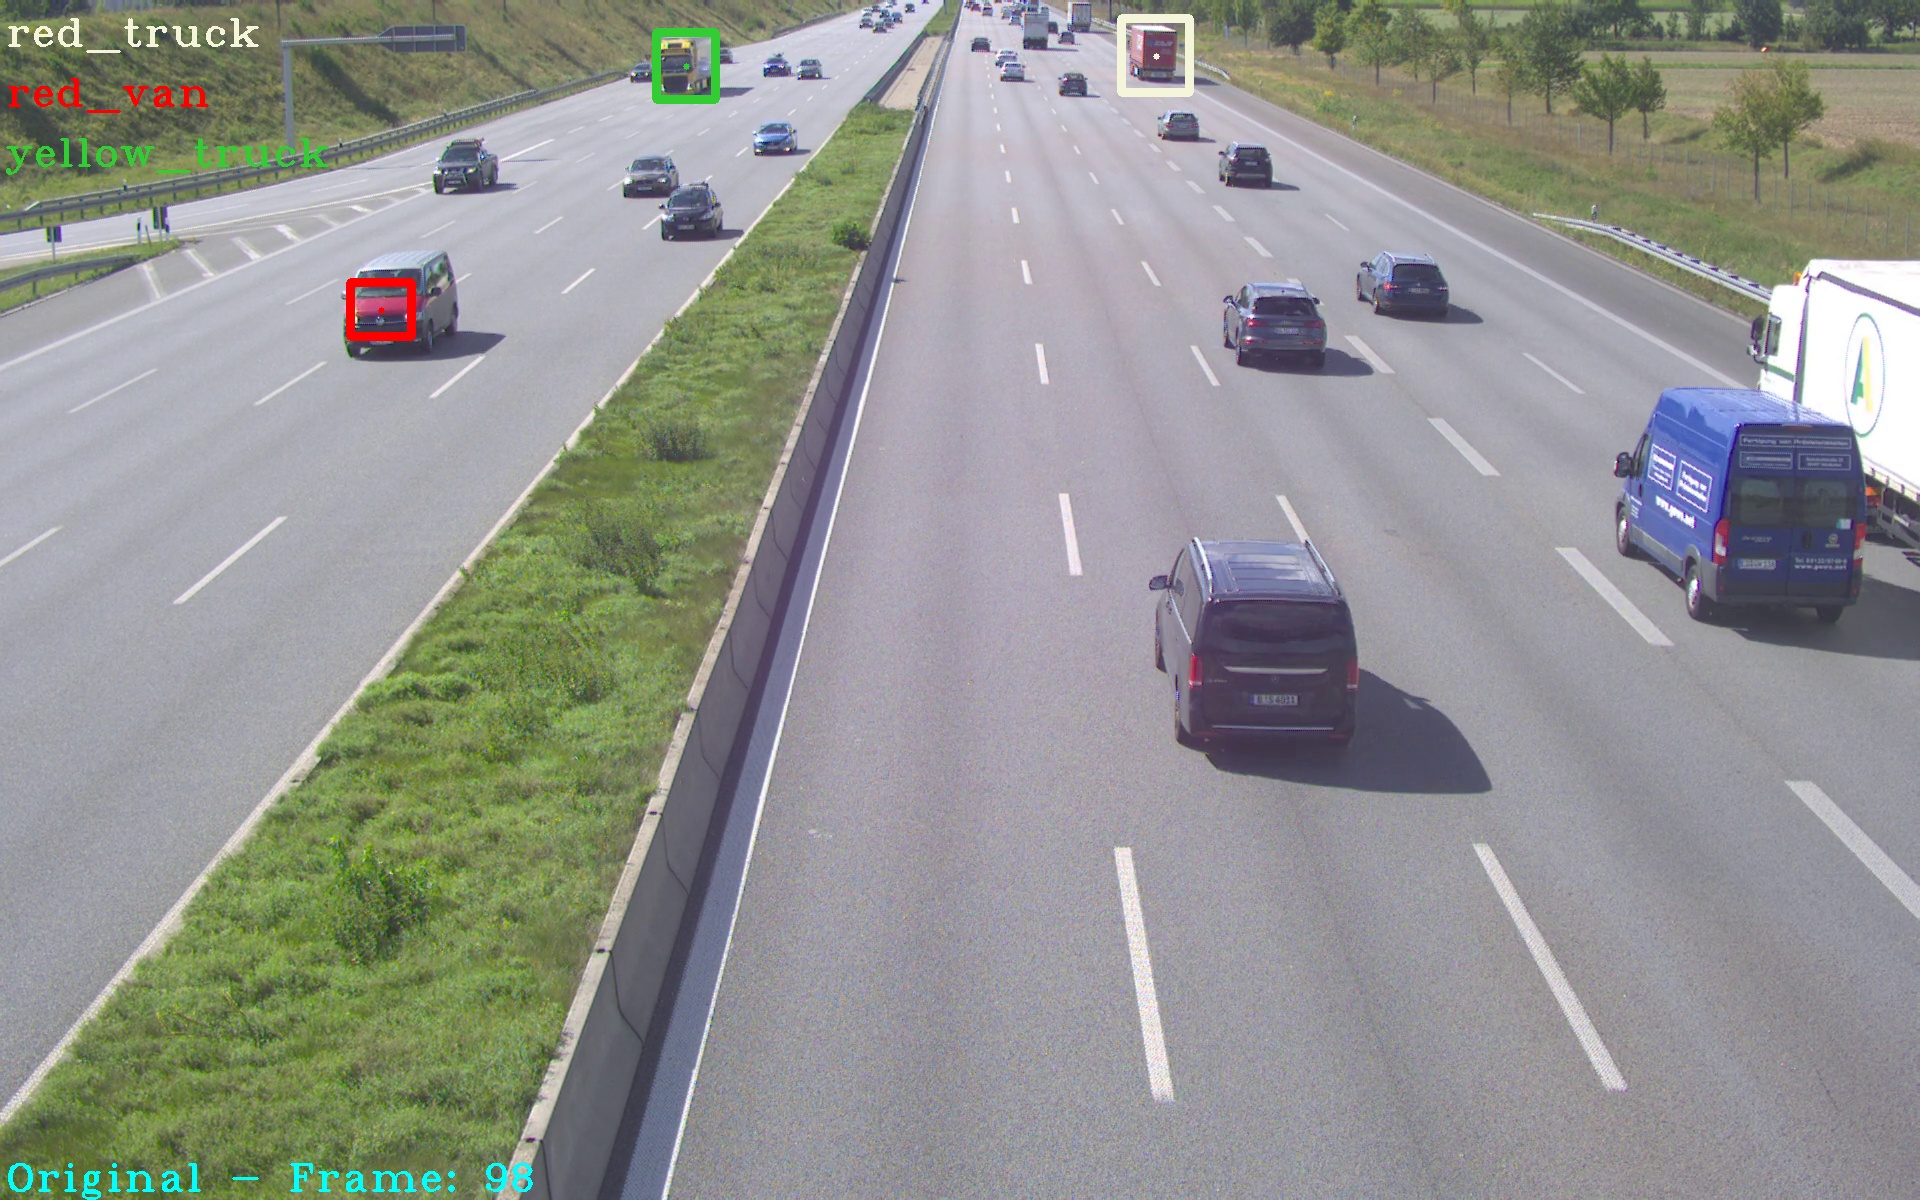
\includegraphics[width=0.45\linewidth]{diagrams/object_tracking/s50_s_near/frame.png}    &  
    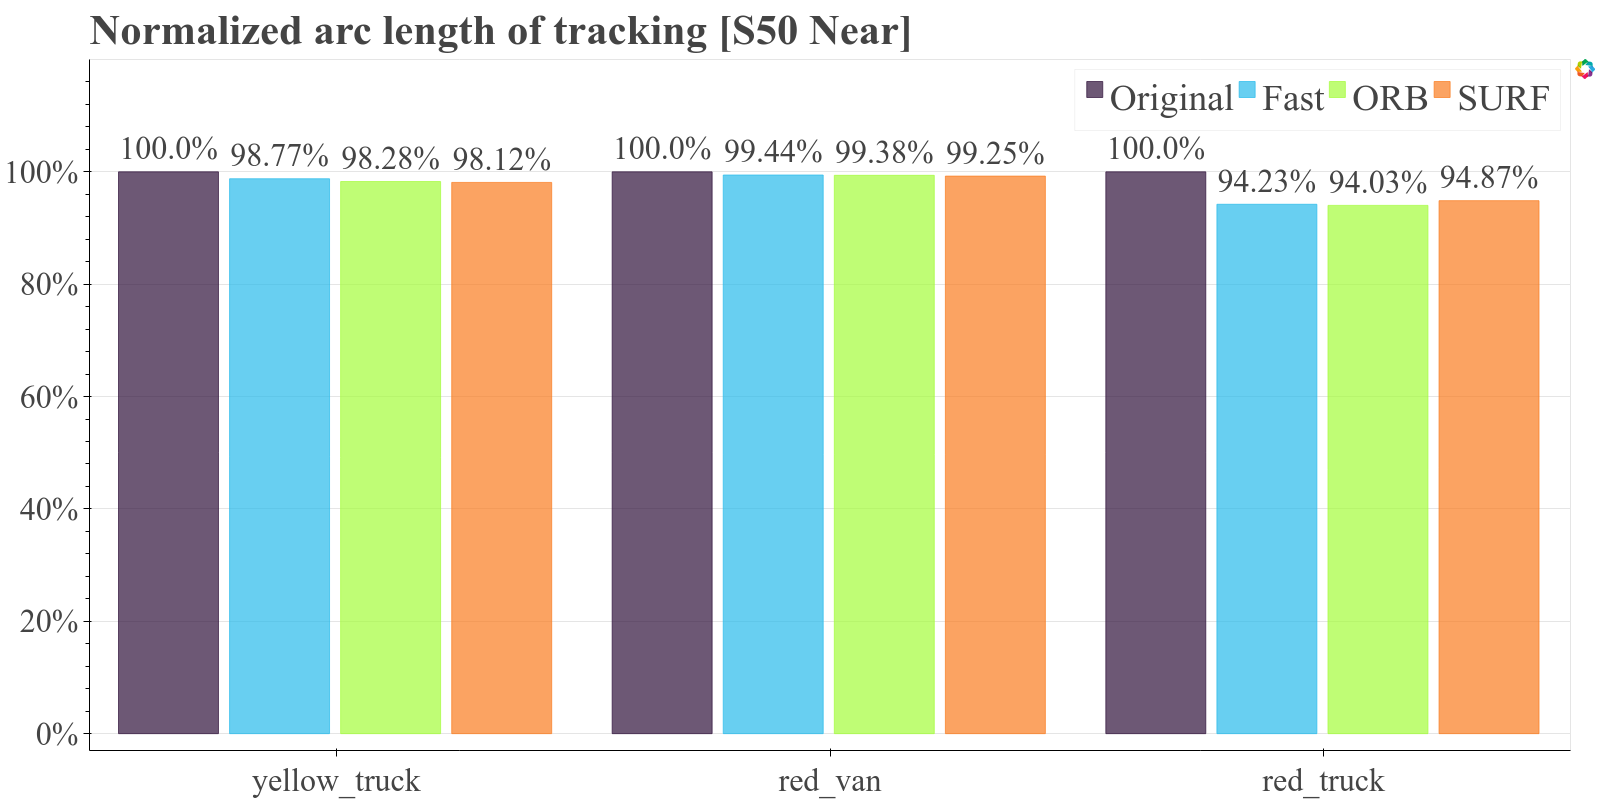
\includegraphics[width=0.475\linewidth]{diagrams/object_tracking/s50_s_near/normalized_arc_lengths.html.png}    \\

    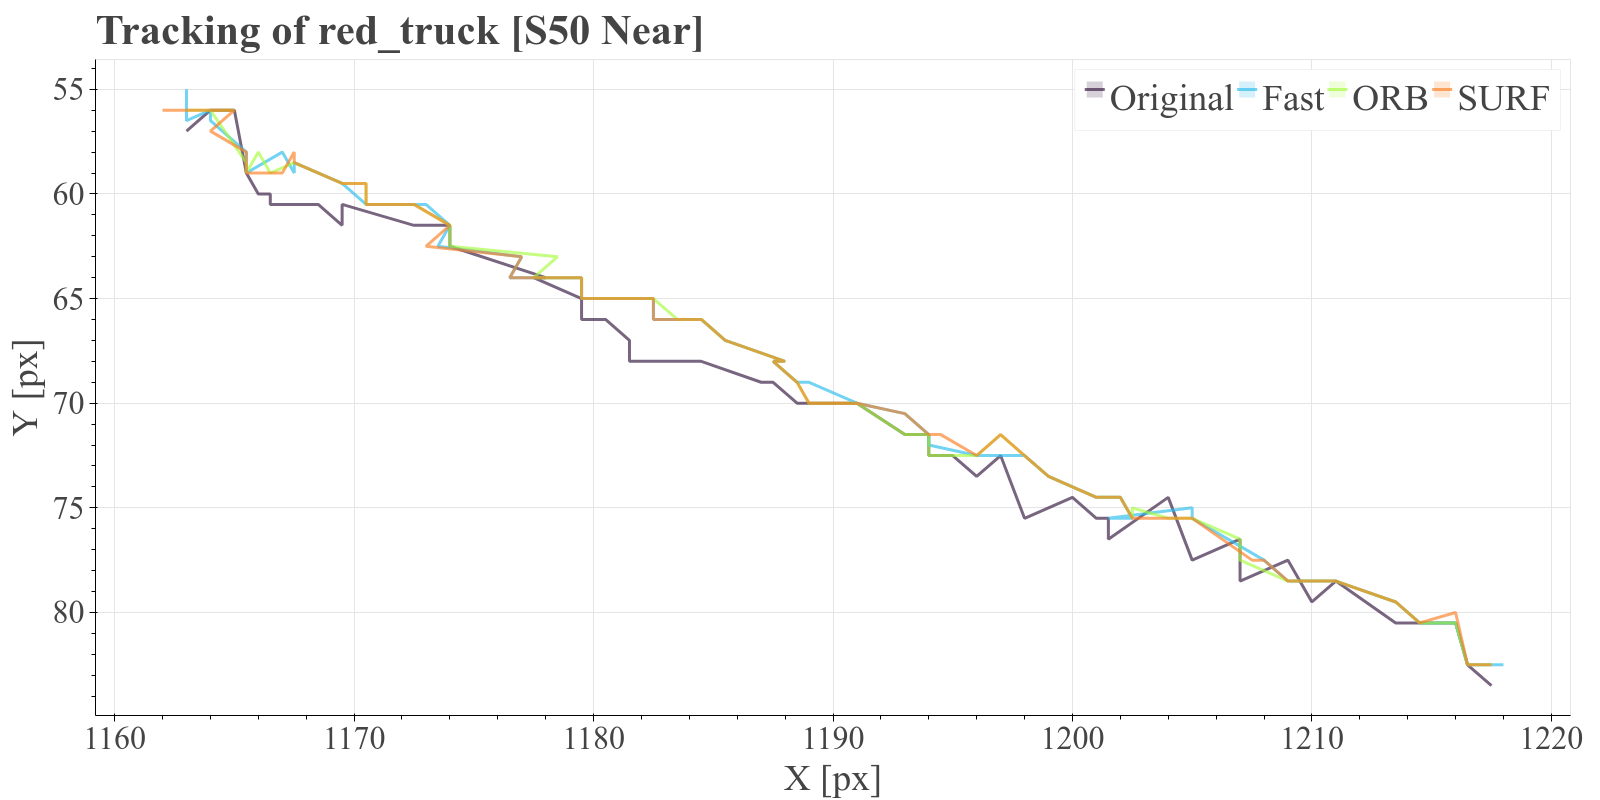
\includegraphics[width=0.475\linewidth]{diagrams/object_tracking/s50_s_near/red_truck.png}    &  
    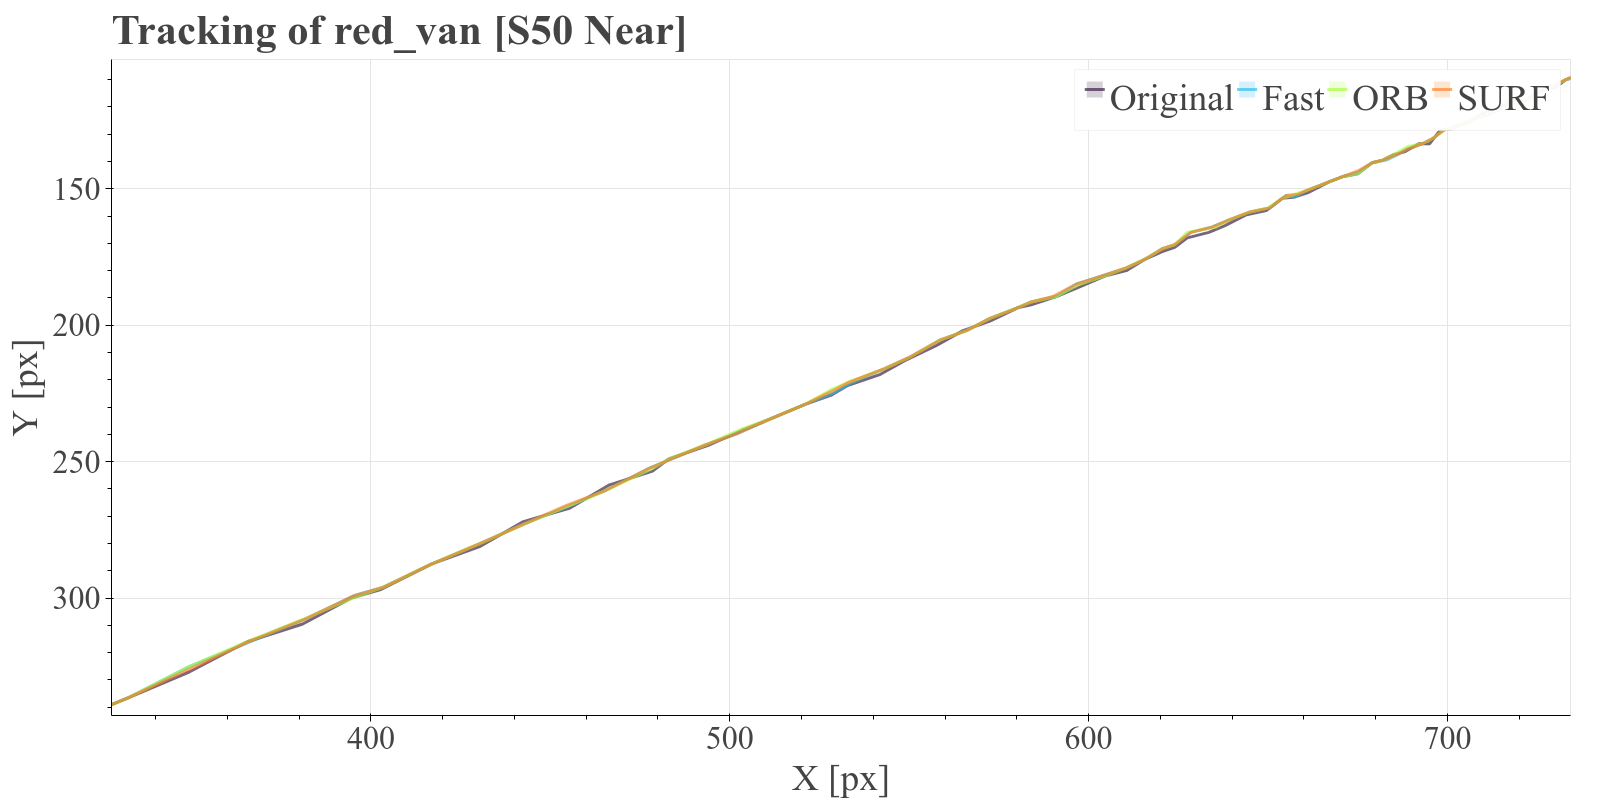
\includegraphics[width=0.475\linewidth]{diagrams/object_tracking/s50_s_near/red_van.png}    \\  
    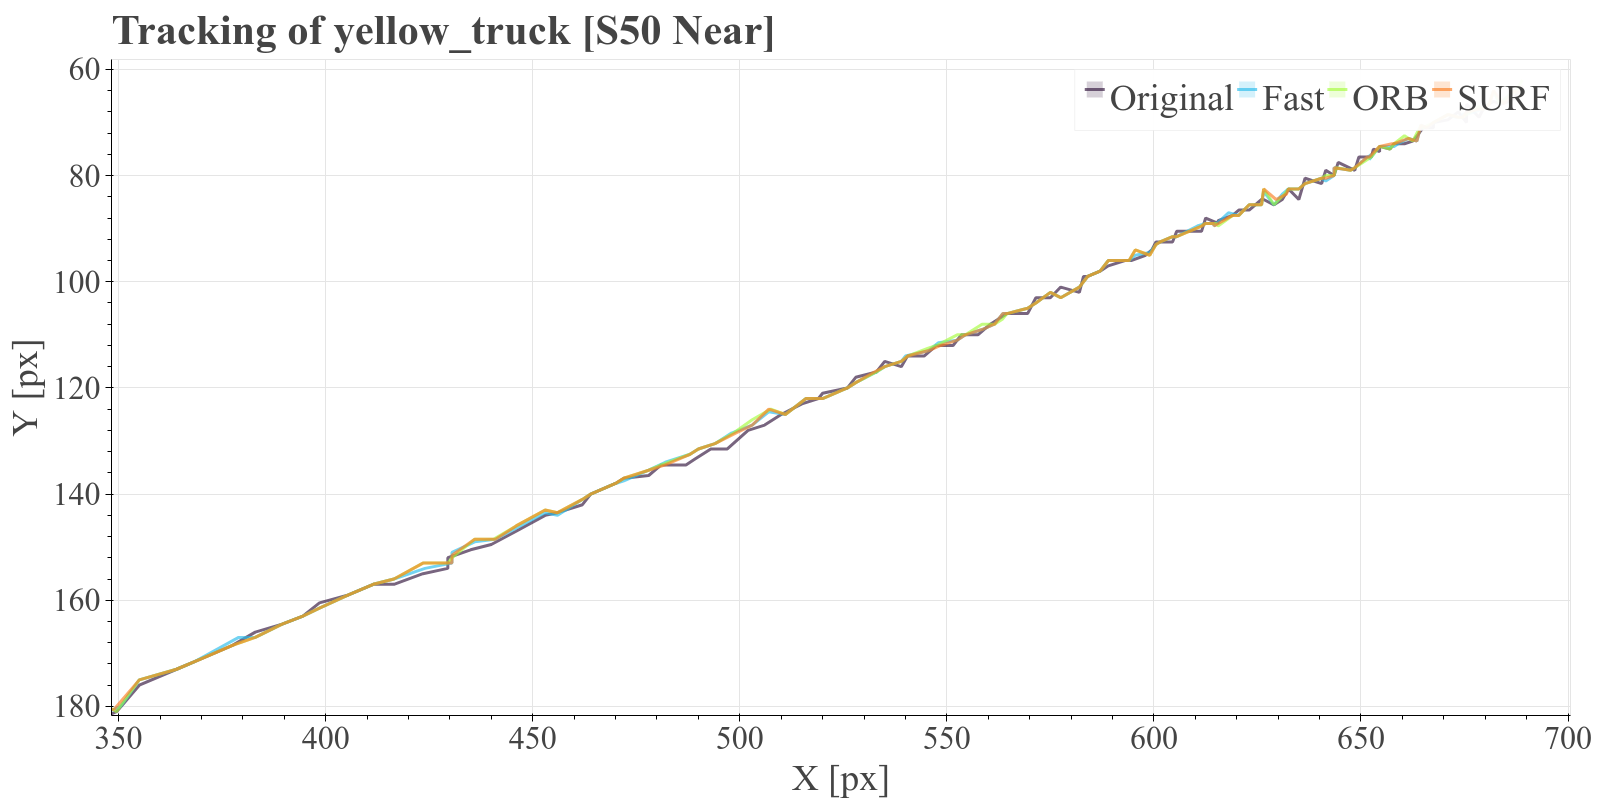
\includegraphics[width=0.475\linewidth]{diagrams/object_tracking/s50_s_near/yellow_truck.png}   
  \end{tabular}
  \caption{Top Left:
  The tracked vehicles in the camera \camsn{5} marked by their bounding boxes. 
  Top right: 
  The normalized arc lengths representing the path of the tracked pixels through the image.
  Bottom graphs:
  The tracked pixel locations of the vehicles as they move through the scene for the original video feed and the stabilized ones.
  It shows that the recording did not include much jitter and thus the paths are already relatively smooth.
  }
  \label{fig:object_tracking_appendix_s50_s_near}
\end{figure*}

\begin{figure*}[!ht]
  \centering
  \begin{tabular}{cc}
    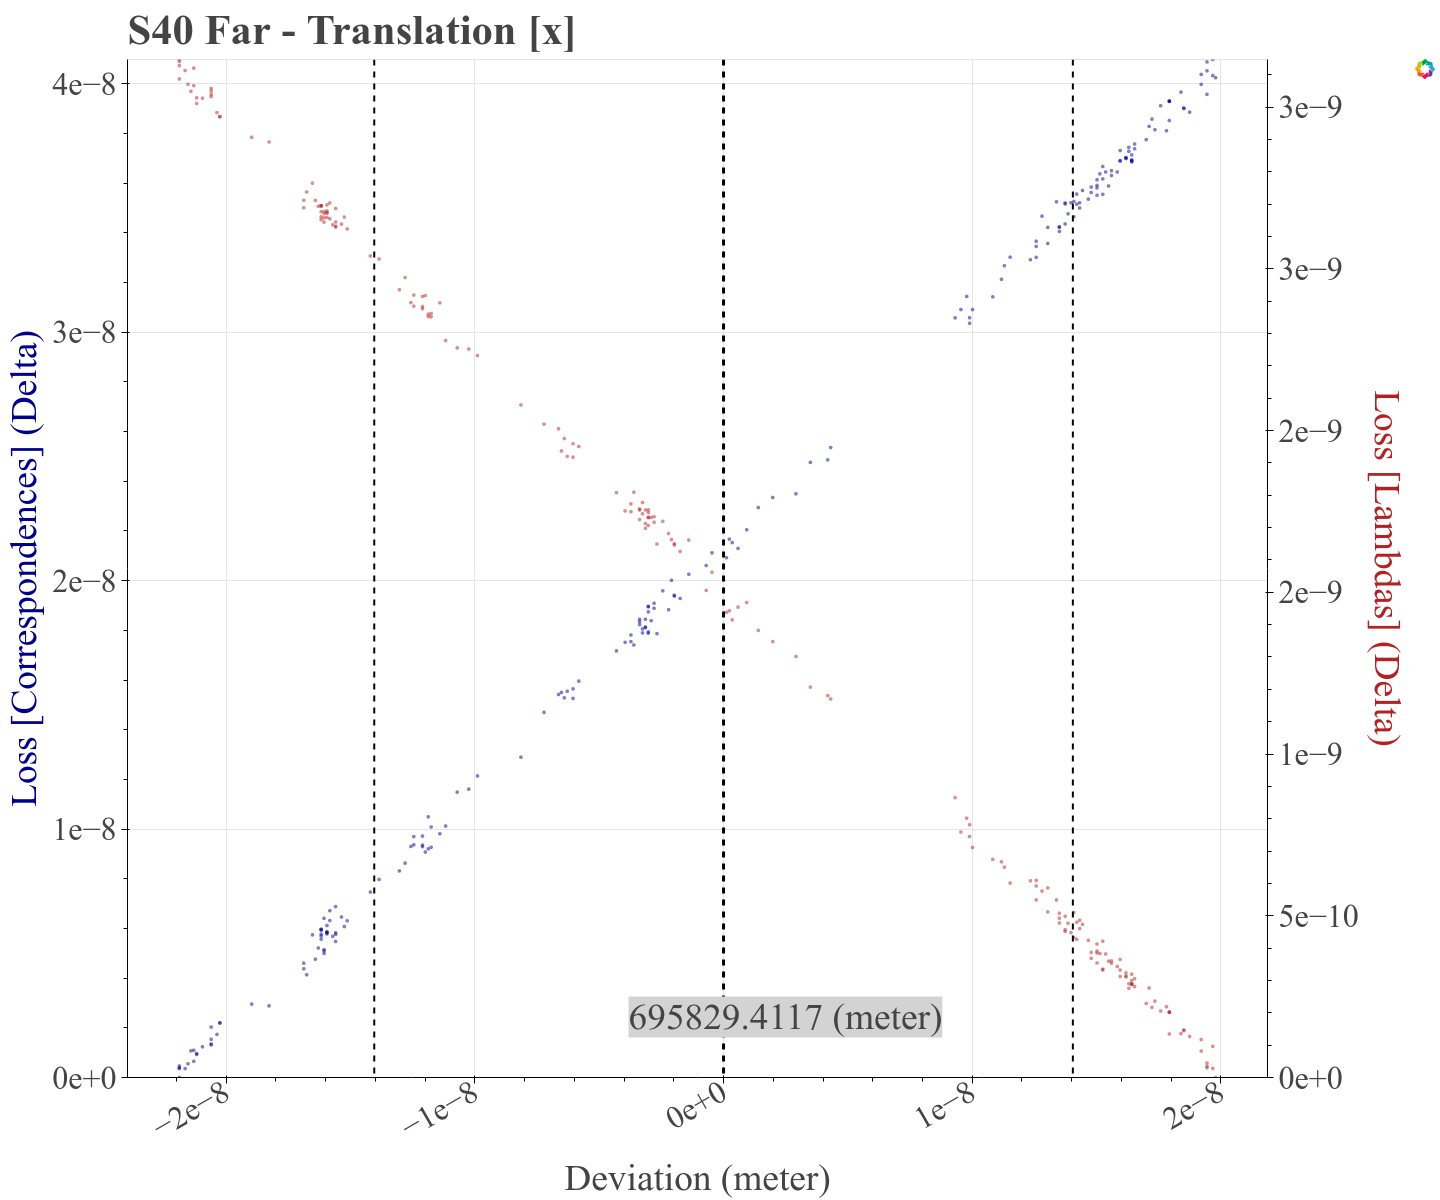
\includegraphics[width=0.45 \linewidth]{diagrams/calibration/s40_n_far/parameters.csv/Translation[x]_vs_Loss[Correspondences]_vs_Loss[Lambdas]_cluster_All.png} &
    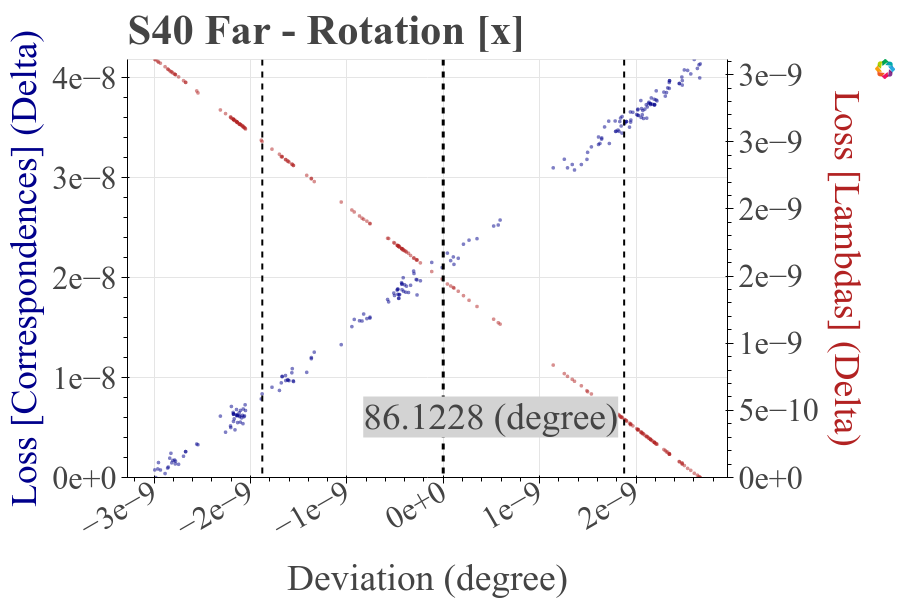
\includegraphics[width=0.45 \linewidth]{diagrams/calibration/s40_n_far/parameters.csv/Rotation[x]_vs_Loss[Correspondences]_vs_Loss[Lambdas]_cluster_All.png} \\
    
    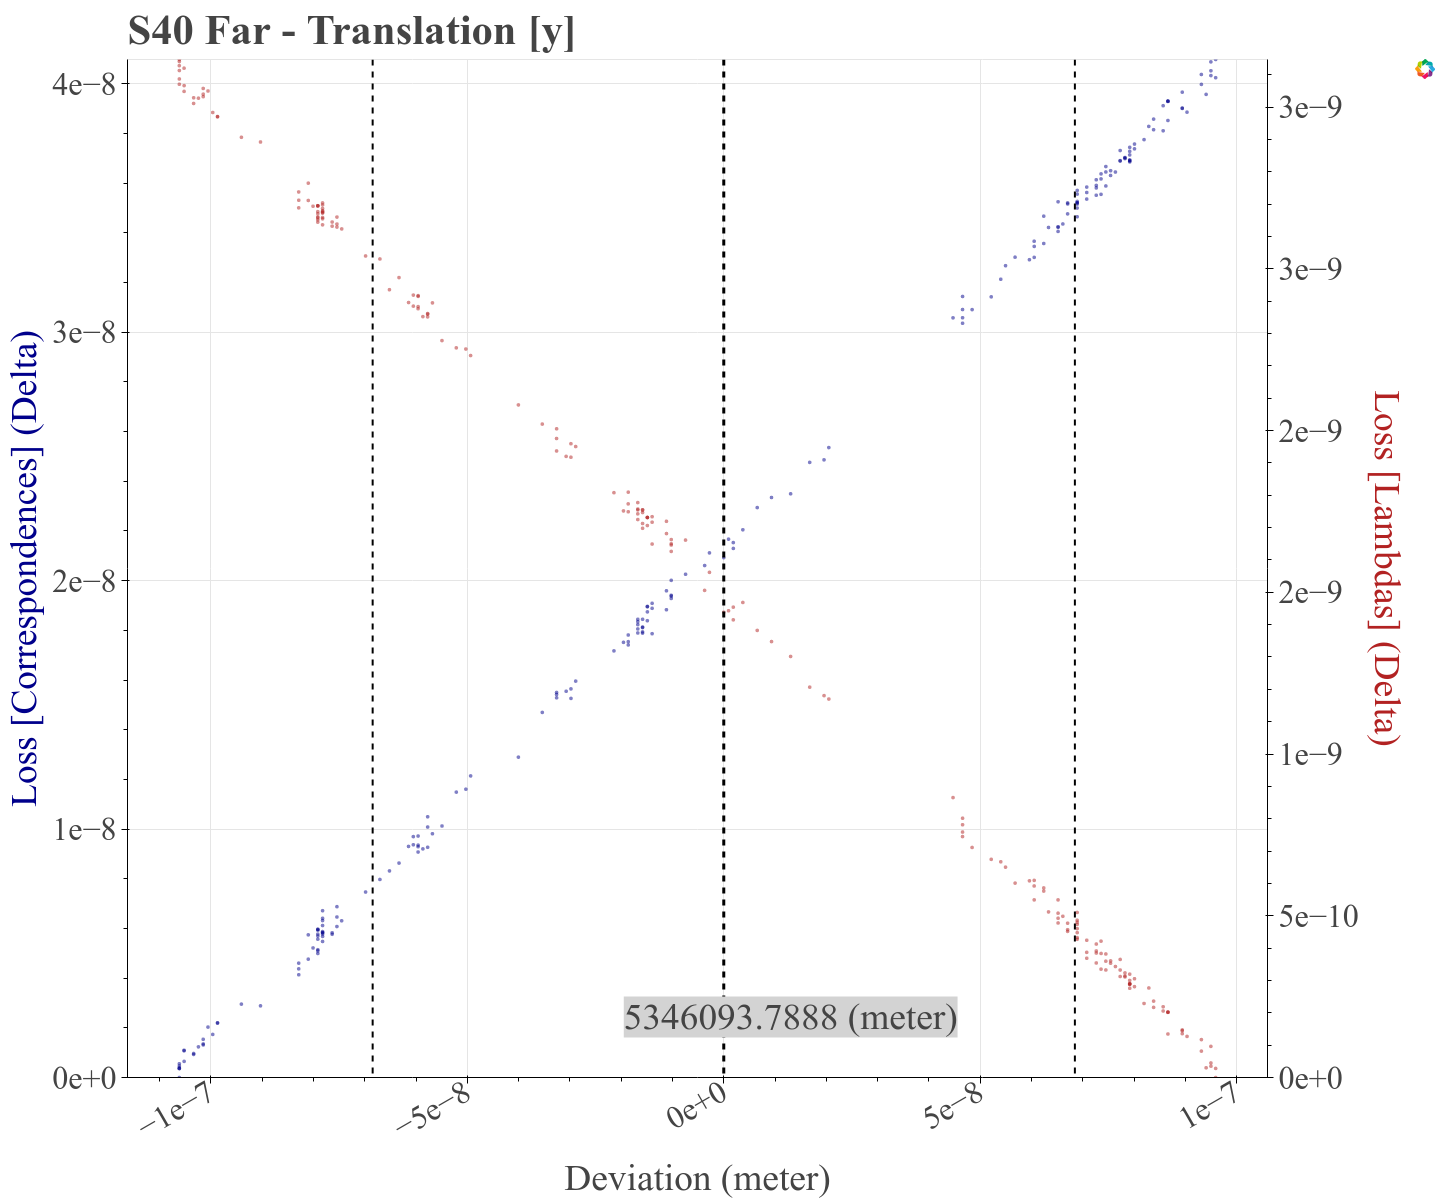
\includegraphics[width=0.45 \linewidth]{diagrams/calibration/s40_n_far/parameters.csv/Translation[y]_vs_Loss[Correspondences]_vs_Loss[Lambdas]_cluster_All.png} &
    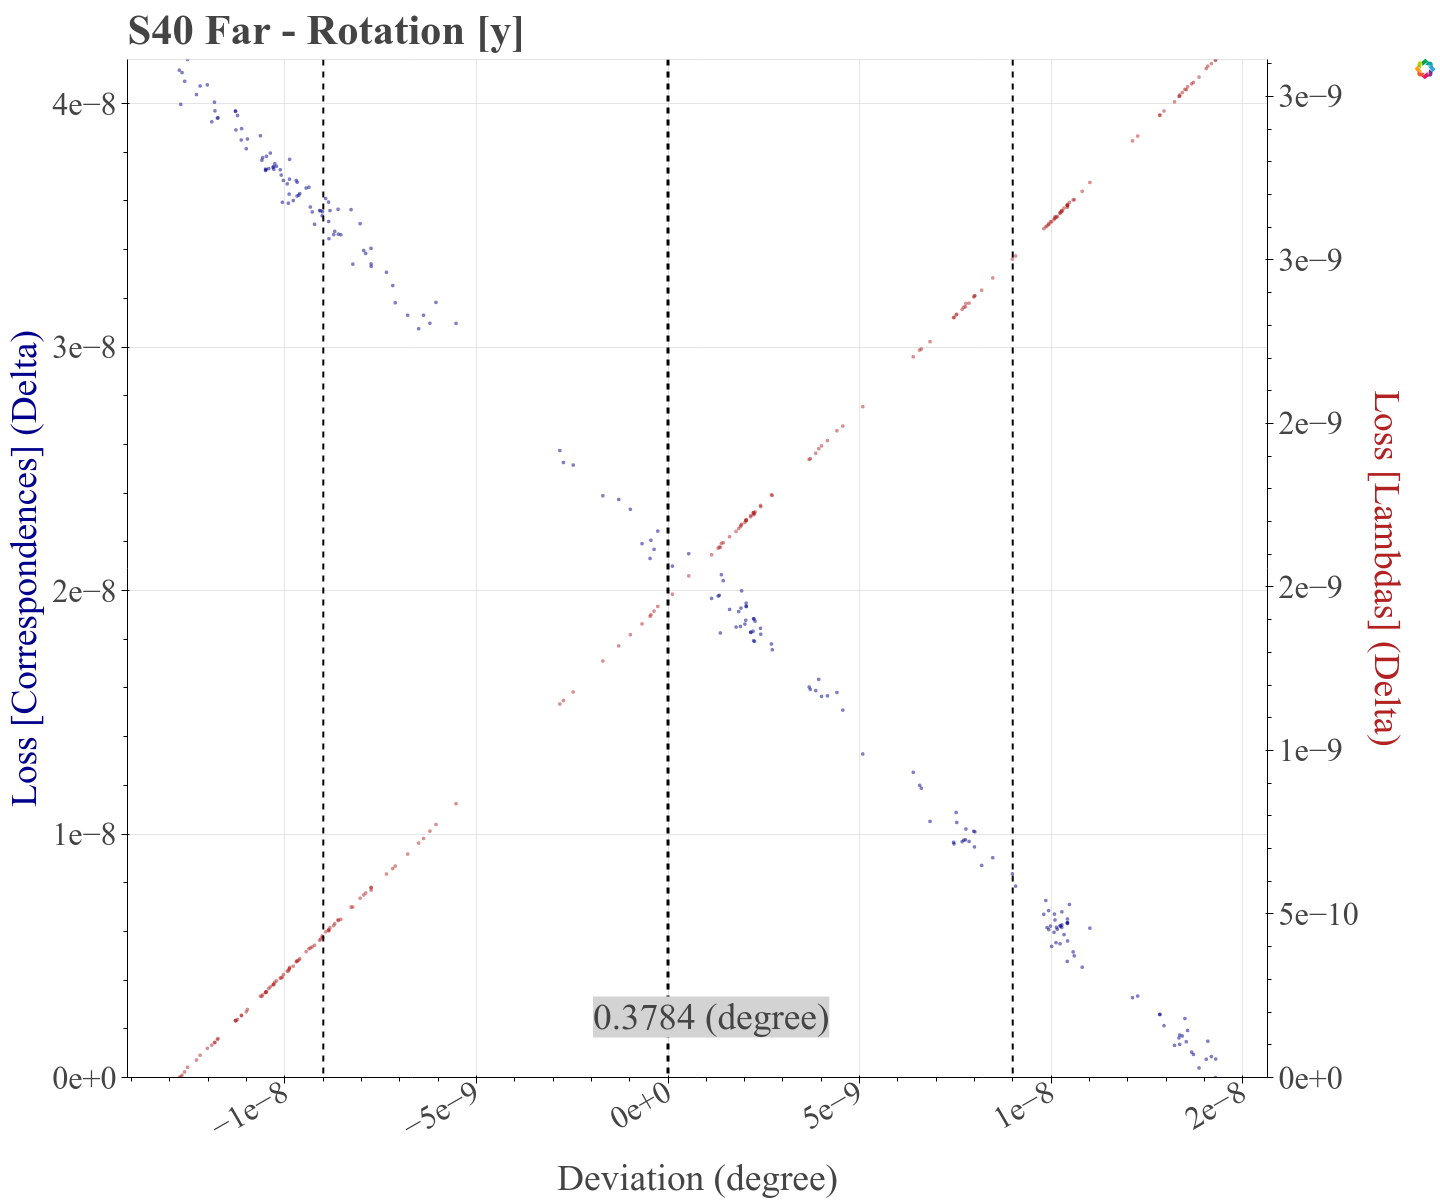
\includegraphics[width=0.45 \linewidth]{diagrams/calibration/s40_n_far/parameters.csv/Rotation[y]_vs_Loss[Correspondences]_vs_Loss[Lambdas]_cluster_All.png} \\
    
    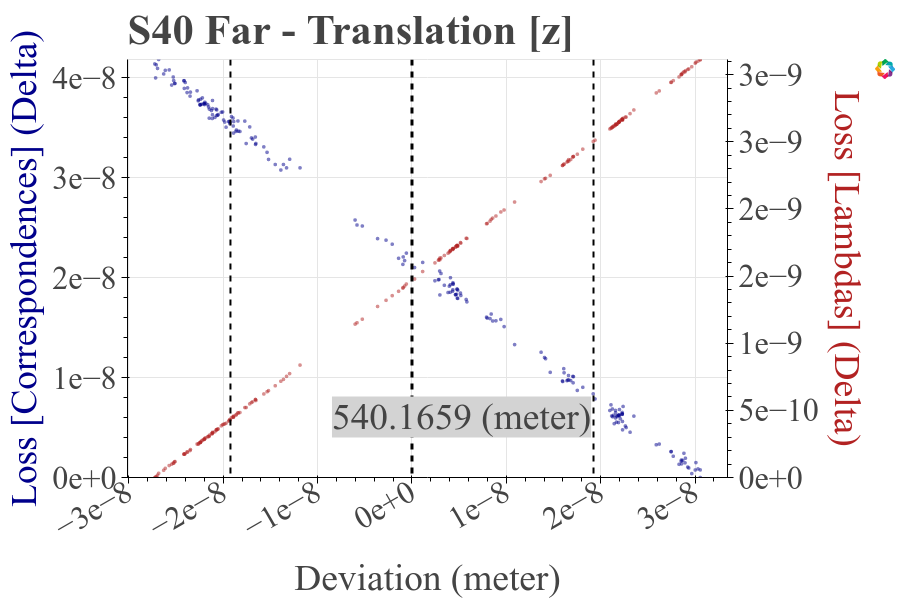
\includegraphics[width=0.45 \linewidth]{diagrams/calibration/s40_n_far/parameters.csv/Translation[z]_vs_Loss[Correspondences]_vs_Loss[Lambdas]_cluster_All.png} &
    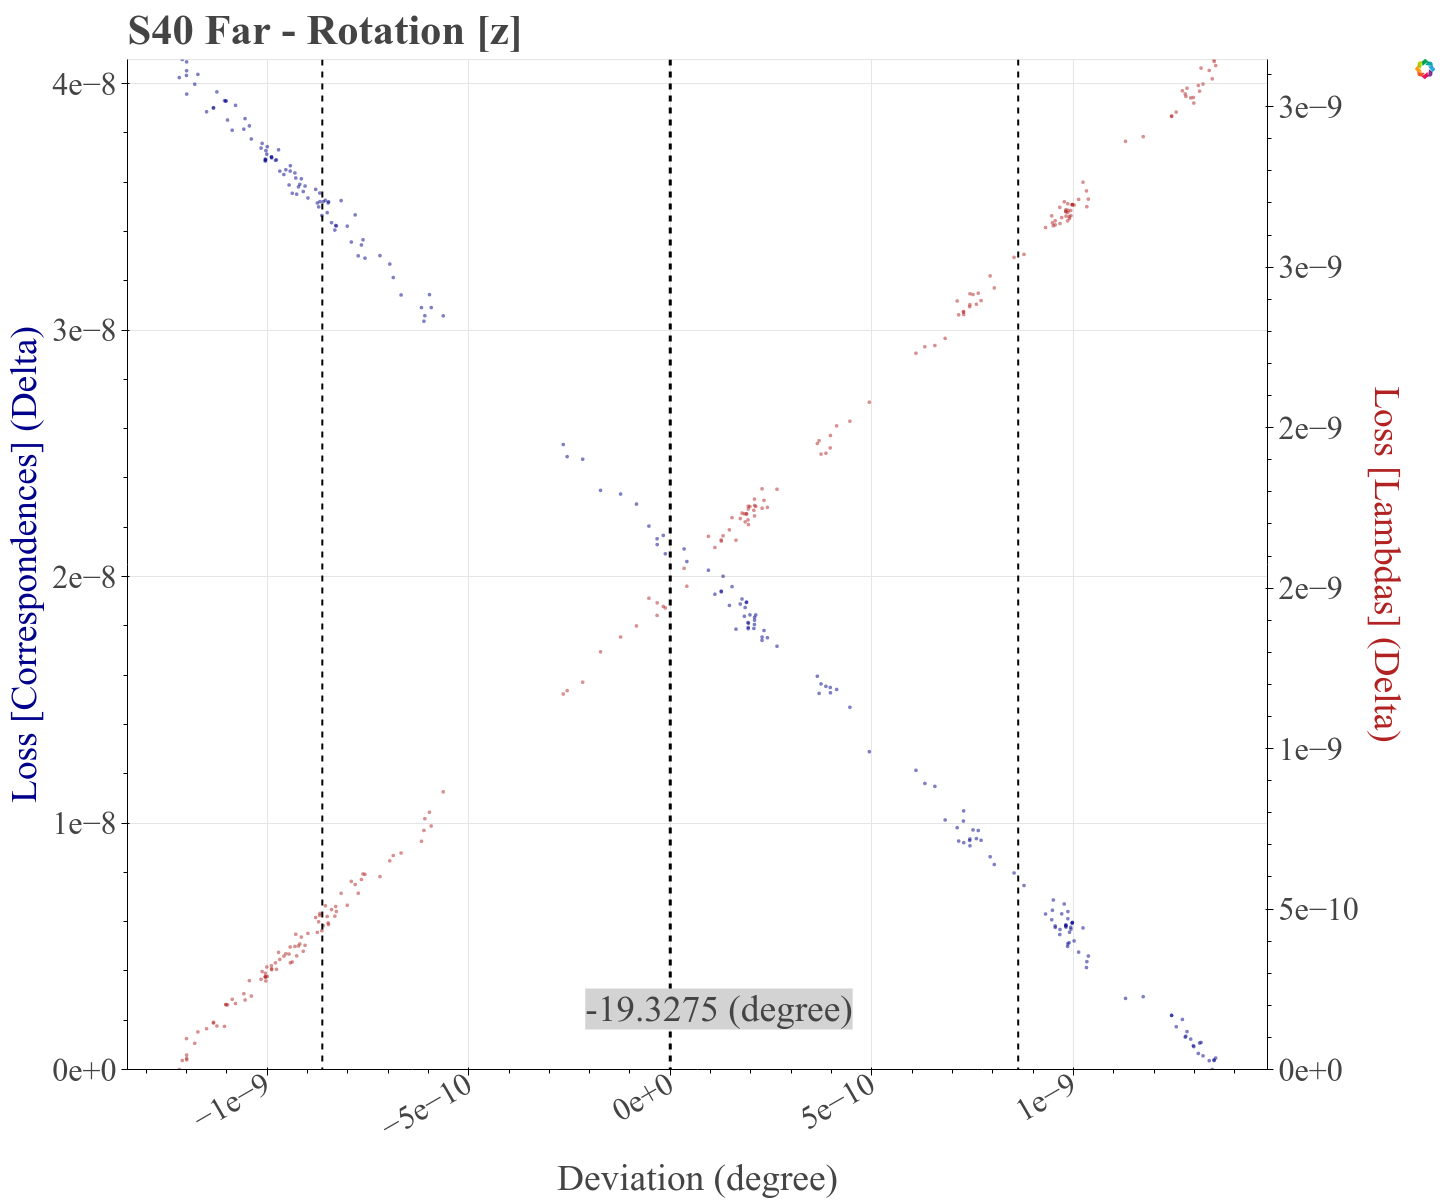
\includegraphics[width=0.45 \linewidth]{diagrams/calibration/s40_n_far/parameters.csv/Rotation[z]_vs_Loss[Correspondences]_vs_Loss[Lambdas]_cluster_All.png} \\

    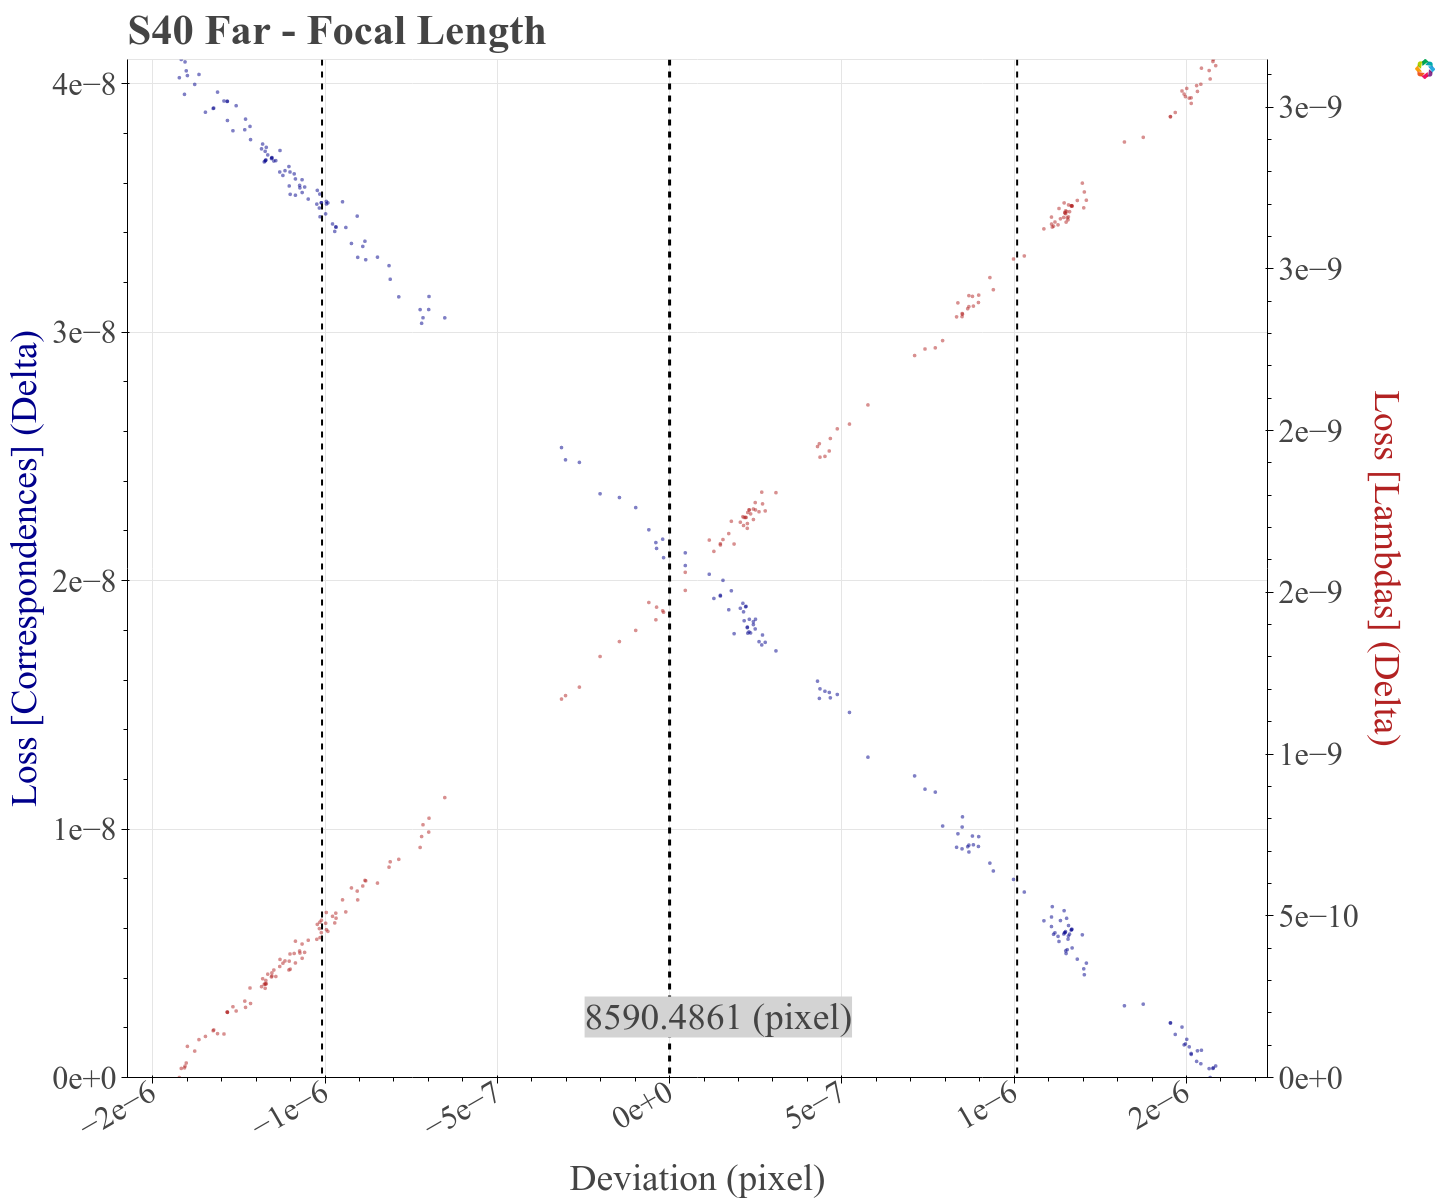
\includegraphics[width=0.45 \linewidth]{diagrams/calibration/s40_n_far/parameters.csv/FocalLength_vs_Loss[Correspondences]_vs_Loss[Lambdas]_cluster_All.png} &
\end{tabular}
\caption{
  Camera: \camsf{4}.
  Left: The resulting translational parameters plotted against the remaining losses. 
  Right: The resulting rotational parameters plotted against the remaining losses.
  Bottom: The resulting focal length  plotted against the remaining losses.
   }
\label{fig:static_calibration_algorithmic_error_s40_n_far}
\end{figure*}

\begin{figure*}[!ht]
  \centering
  \begin{tabular}{cc}
    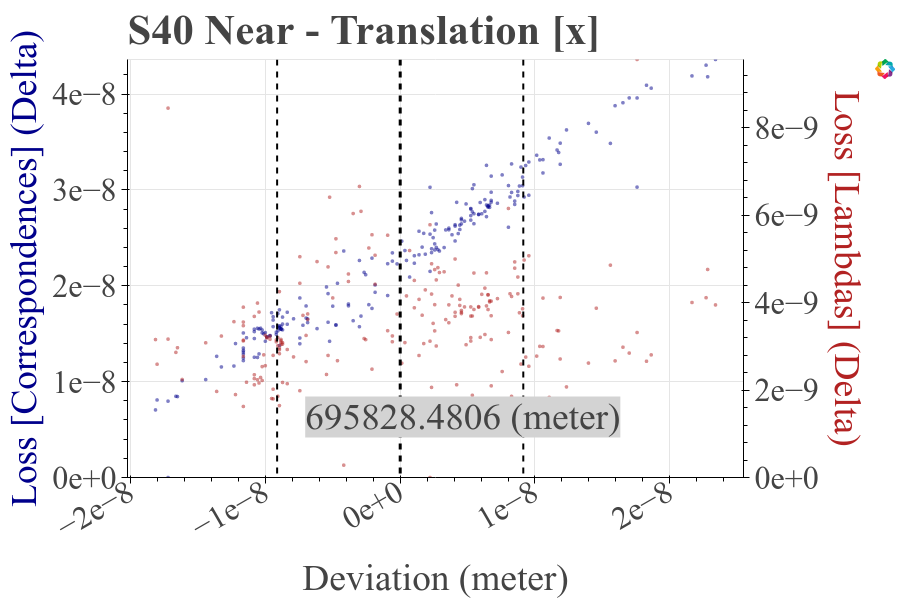
\includegraphics[width=0.45 \linewidth]{diagrams/calibration/s40_n_near/parameters.csv/Translation[x]_vs_Loss[Correspondences]_vs_Loss[Lambdas]_cluster_All.png} &
    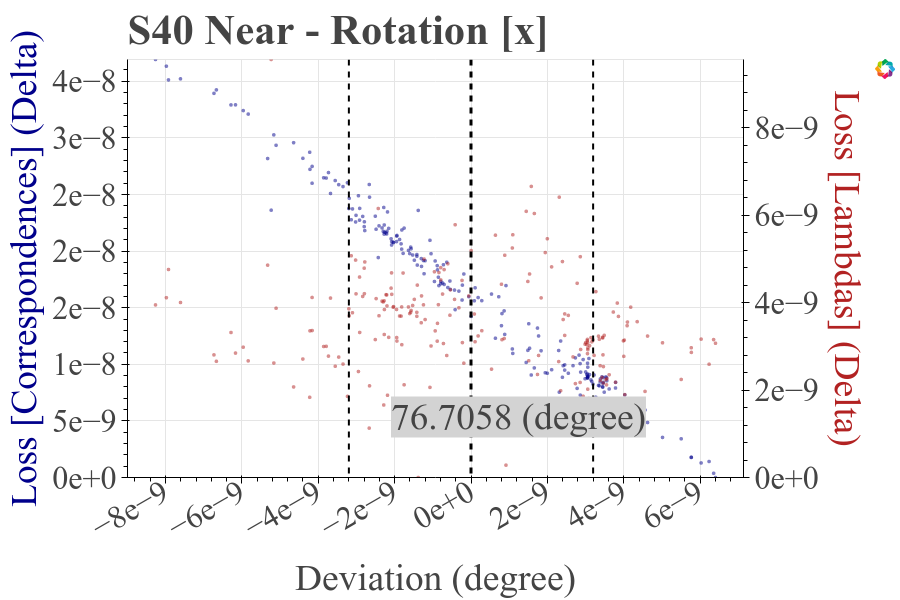
\includegraphics[width=0.45 \linewidth]{diagrams/calibration/s40_n_near/parameters.csv/Rotation[x]_vs_Loss[Correspondences]_vs_Loss[Lambdas]_cluster_All.png} \\
    
    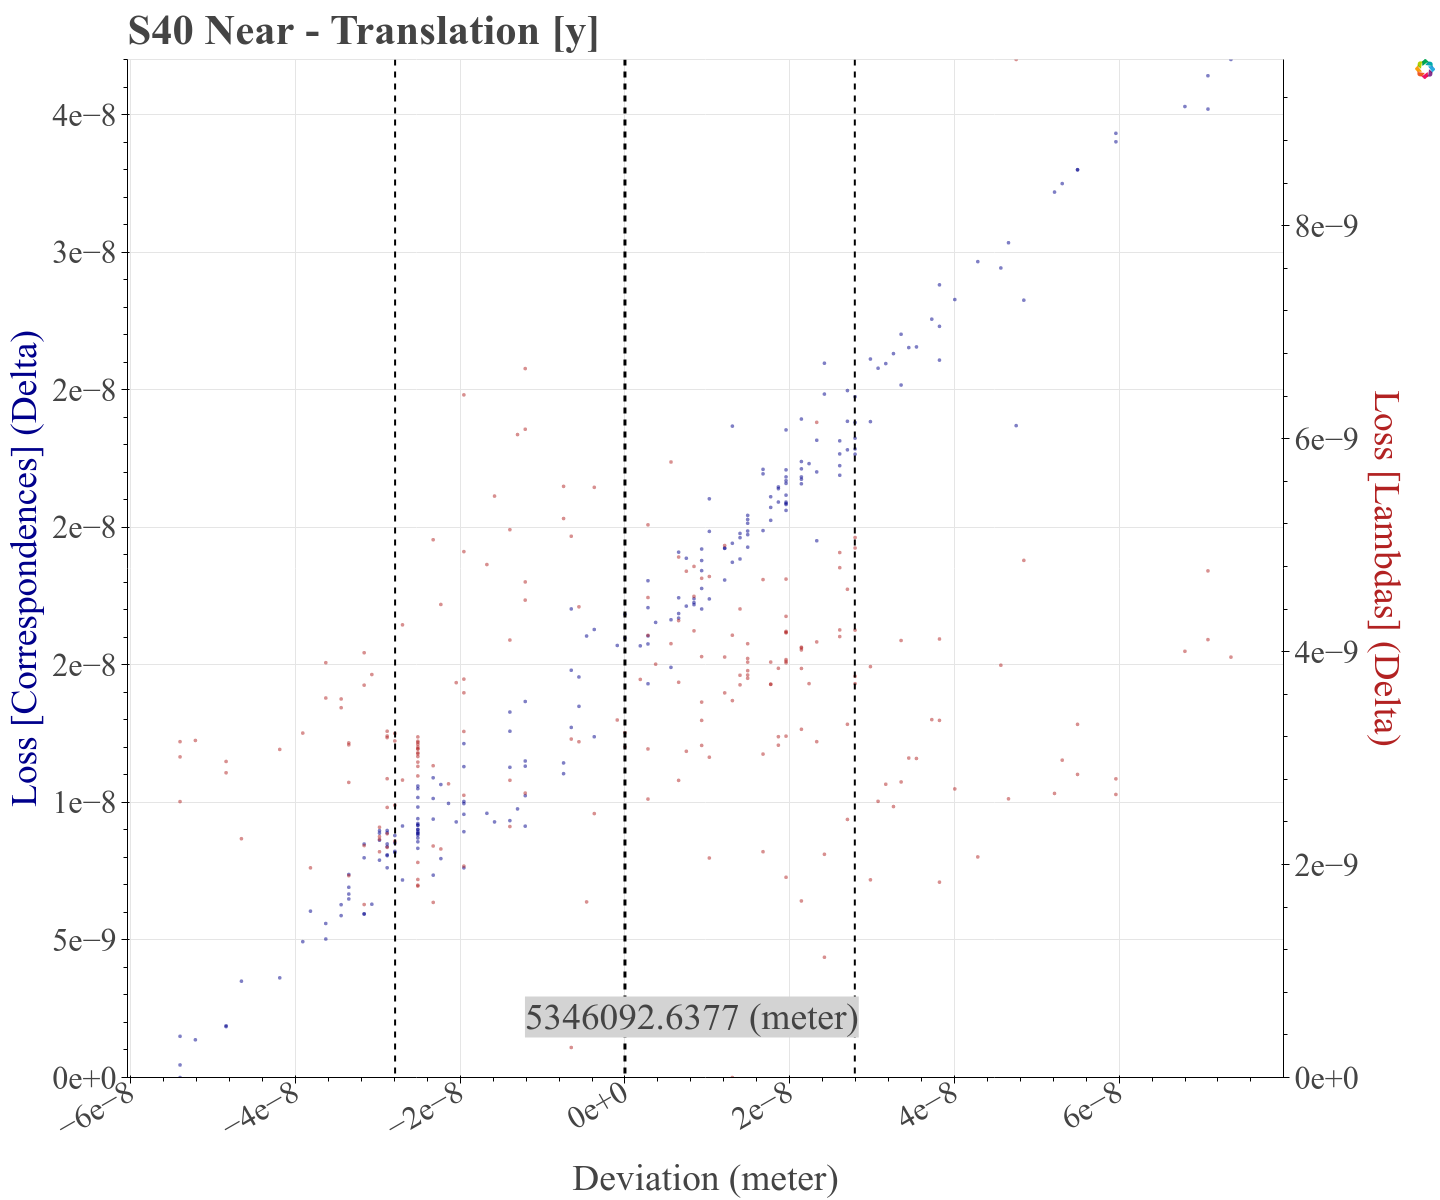
\includegraphics[width=0.45 \linewidth]{diagrams/calibration/s40_n_near/parameters.csv/Translation[y]_vs_Loss[Correspondences]_vs_Loss[Lambdas]_cluster_All.png} &
    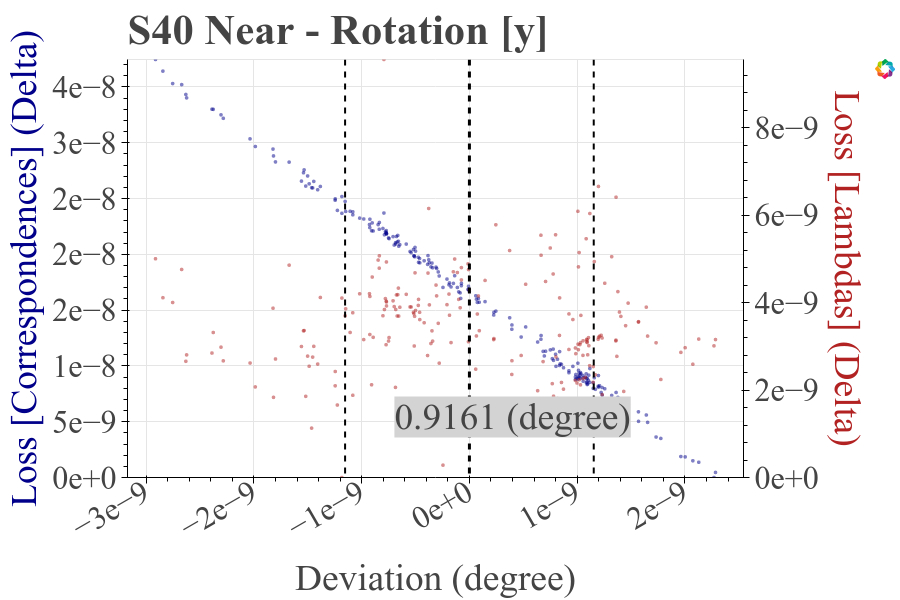
\includegraphics[width=0.45 \linewidth]{diagrams/calibration/s40_n_near/parameters.csv/Rotation[y]_vs_Loss[Correspondences]_vs_Loss[Lambdas]_cluster_All.png} \\
    
    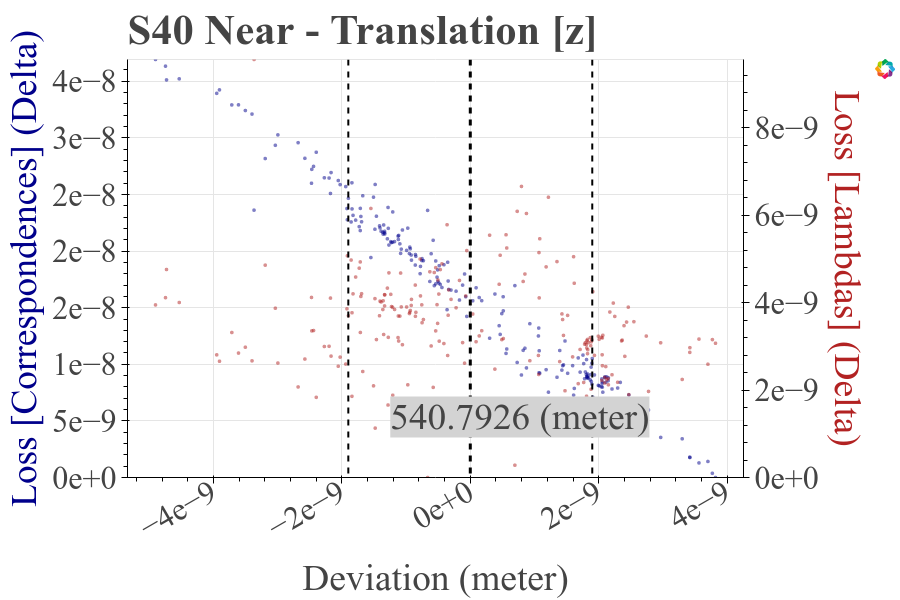
\includegraphics[width=0.45 \linewidth]{diagrams/calibration/s40_n_near/parameters.csv/Translation[z]_vs_Loss[Correspondences]_vs_Loss[Lambdas]_cluster_All.png} &
    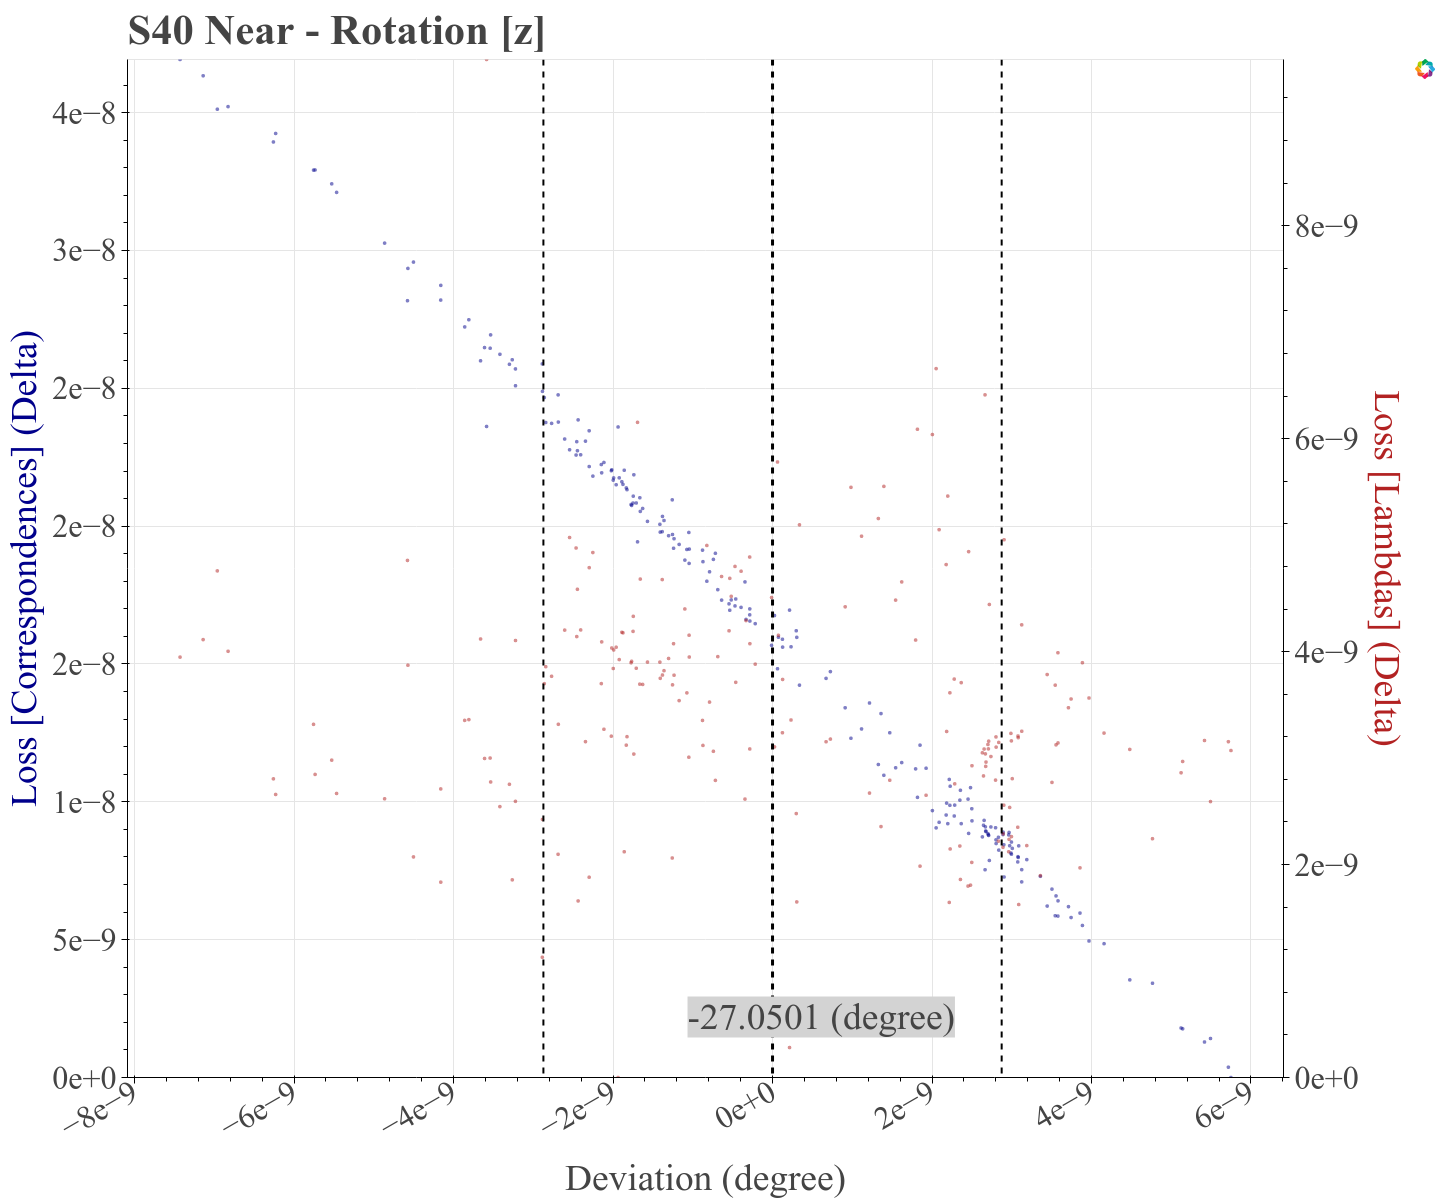
\includegraphics[width=0.45 \linewidth]{diagrams/calibration/s40_n_near/parameters.csv/Rotation[z]_vs_Loss[Correspondences]_vs_Loss[Lambdas]_cluster_All.png} \\

    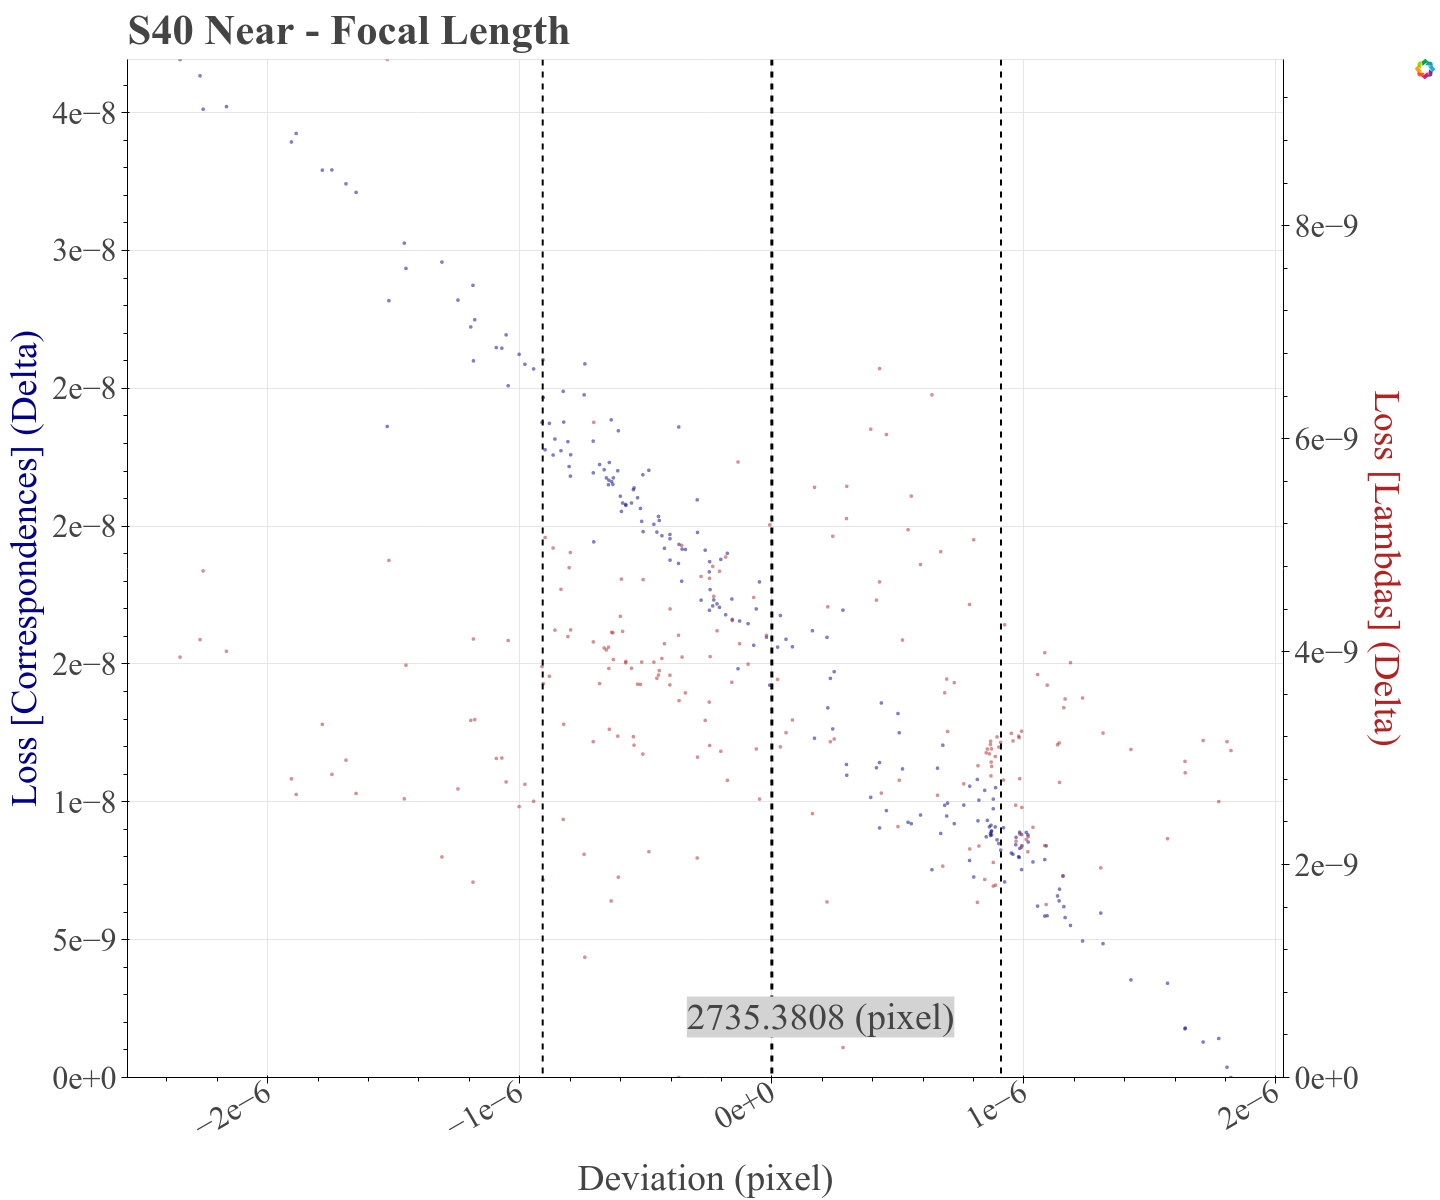
\includegraphics[width=0.45 \linewidth]{diagrams/calibration/s40_n_near/parameters.csv/FocalLength_vs_Loss[Correspondences]_vs_Loss[Lambdas]_cluster_All.png} &
\end{tabular}
\caption{
  Camera: \camsn{4}.
  Left: The resulting translational parameters plotted against the remaining losses. 
  Right: The resulting rotational parameters plotted against the remaining losses.
  Bottom: The resulting focal length  plotted against the remaining losses.
     }
\label{fig:static_calibration_algorithmic_error_s40_n_near}
\end{figure*}

\begin{figure*}[!ht]
  \centering
  \begin{tabular}{cc}
    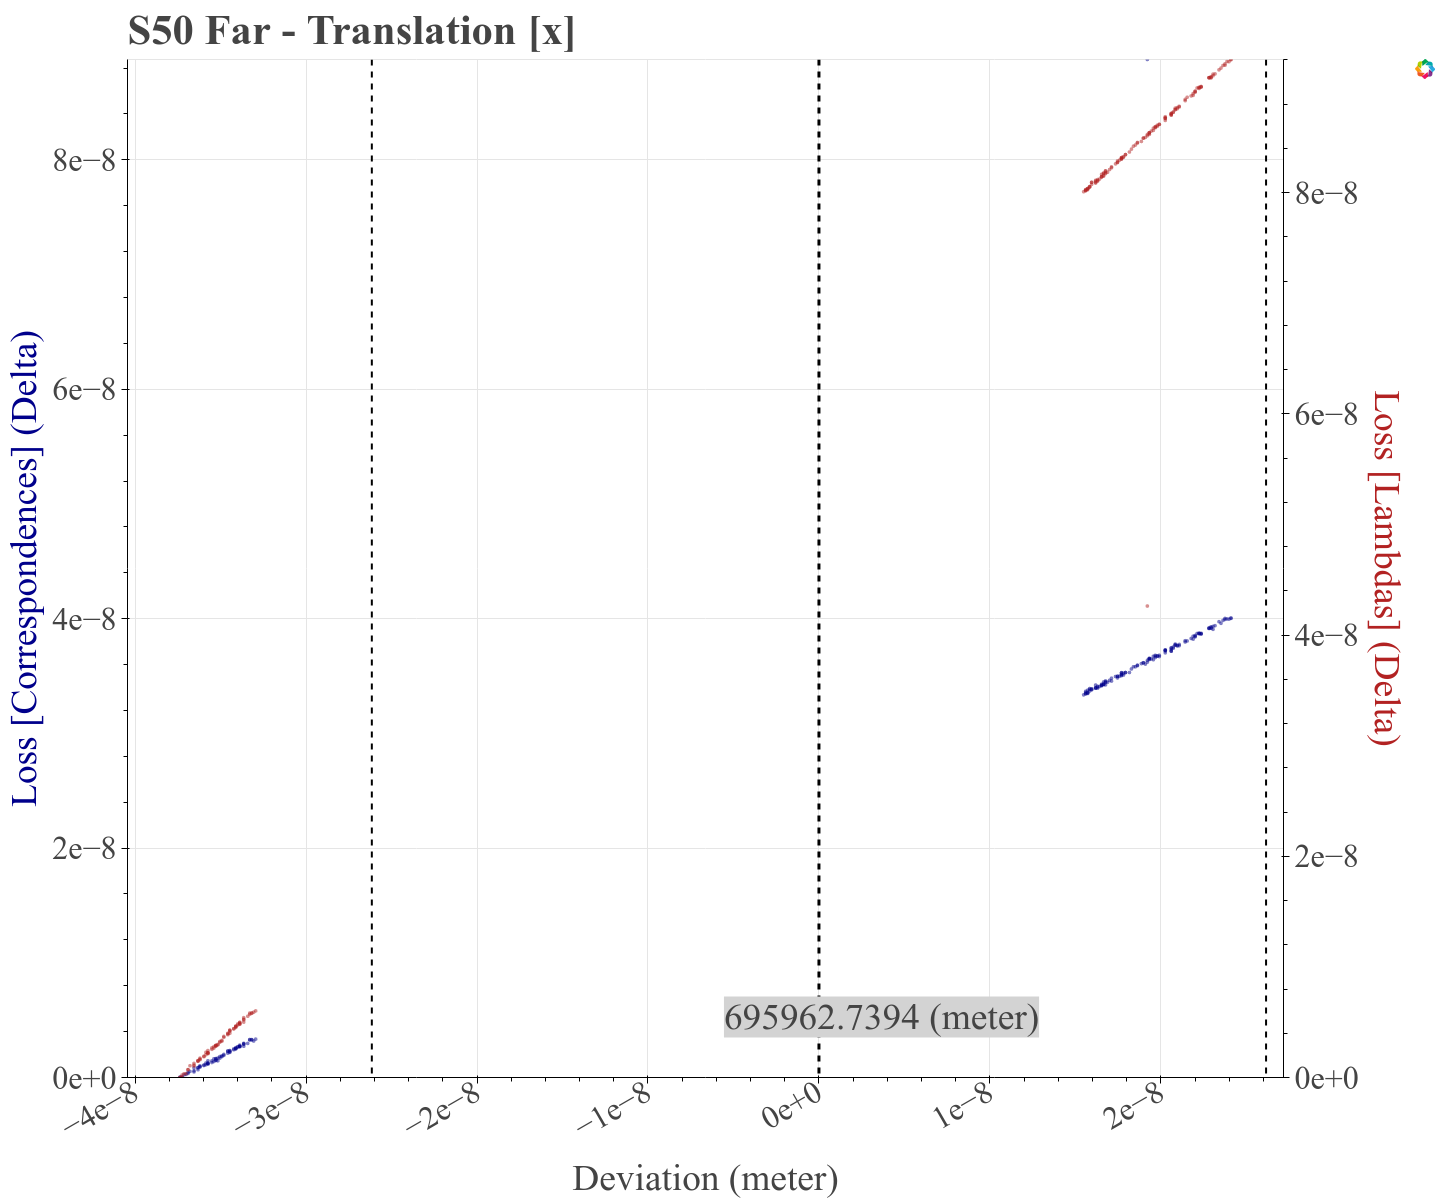
\includegraphics[width=0.45 \linewidth]{diagrams/calibration/s50_s_far/parameters.csv/Translation[x]_vs_Loss[Correspondences]_vs_Loss[Lambdas]_cluster_All.png} &
    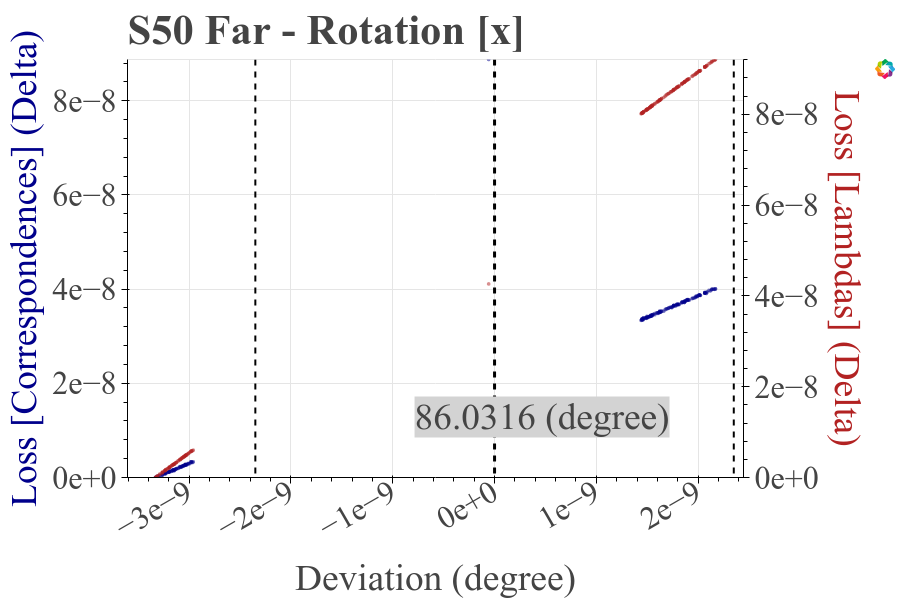
\includegraphics[width=0.45 \linewidth]{diagrams/calibration/s50_s_far/parameters.csv/Rotation[x]_vs_Loss[Correspondences]_vs_Loss[Lambdas]_cluster_All.png} \\
    
    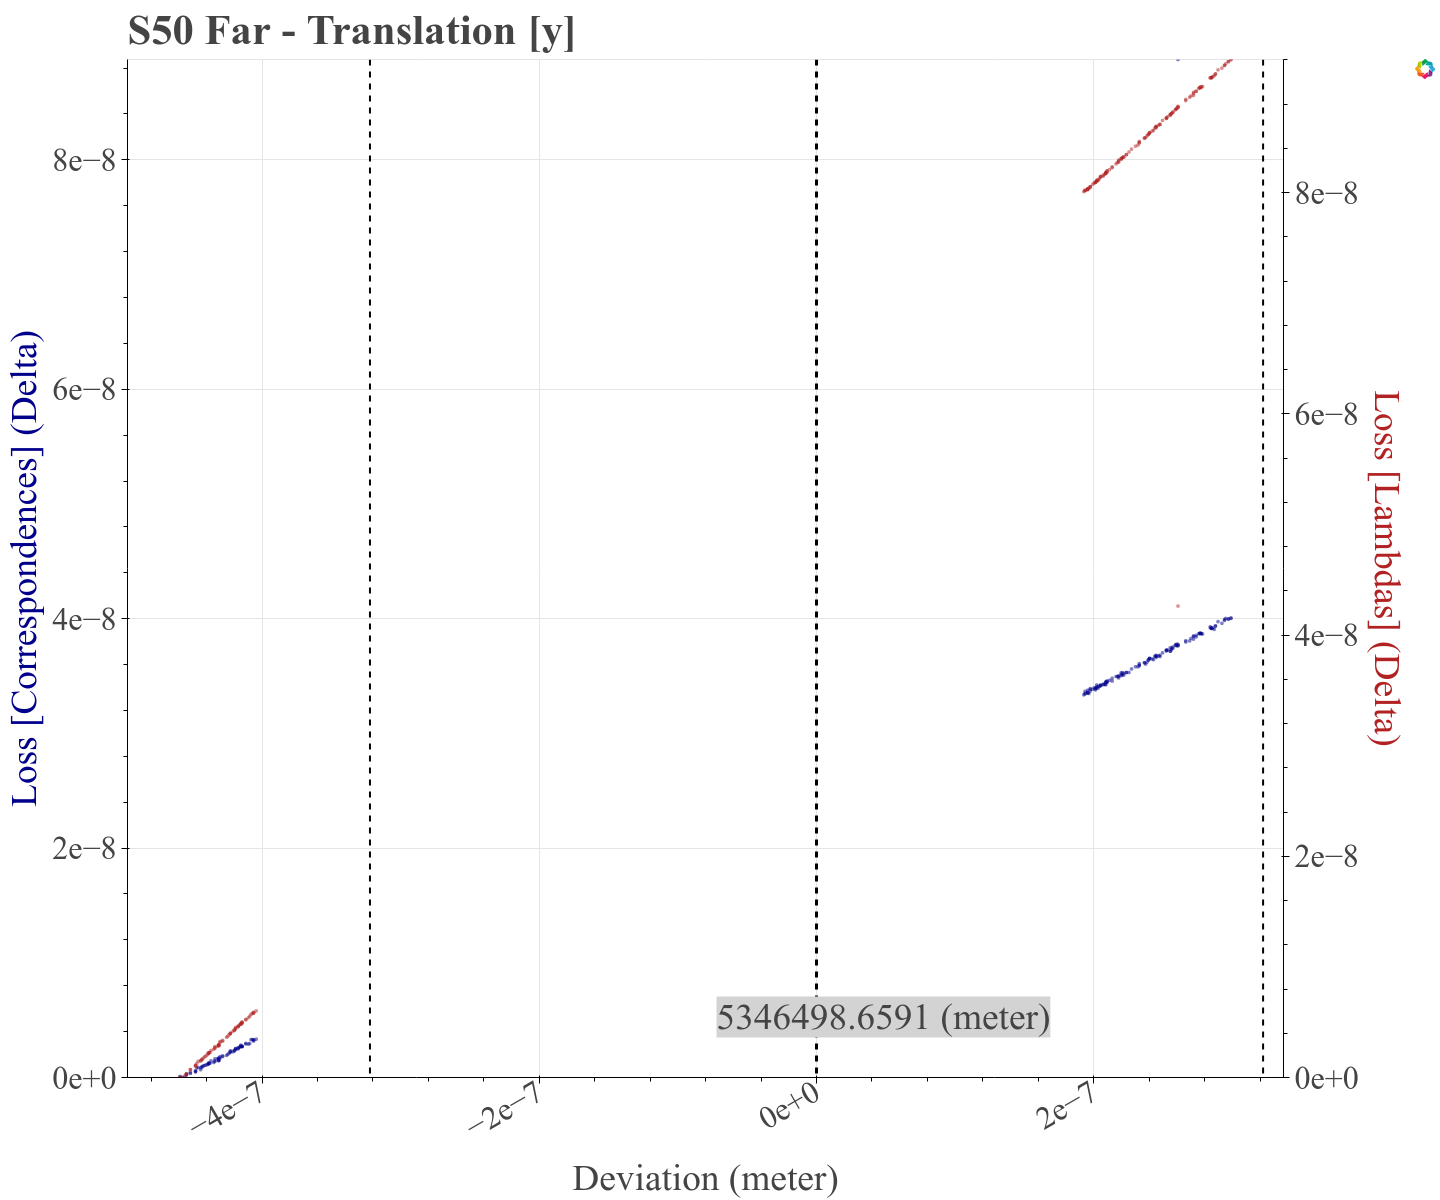
\includegraphics[width=0.45 \linewidth]{diagrams/calibration/s50_s_far/parameters.csv/Translation[y]_vs_Loss[Correspondences]_vs_Loss[Lambdas]_cluster_All.png} &
    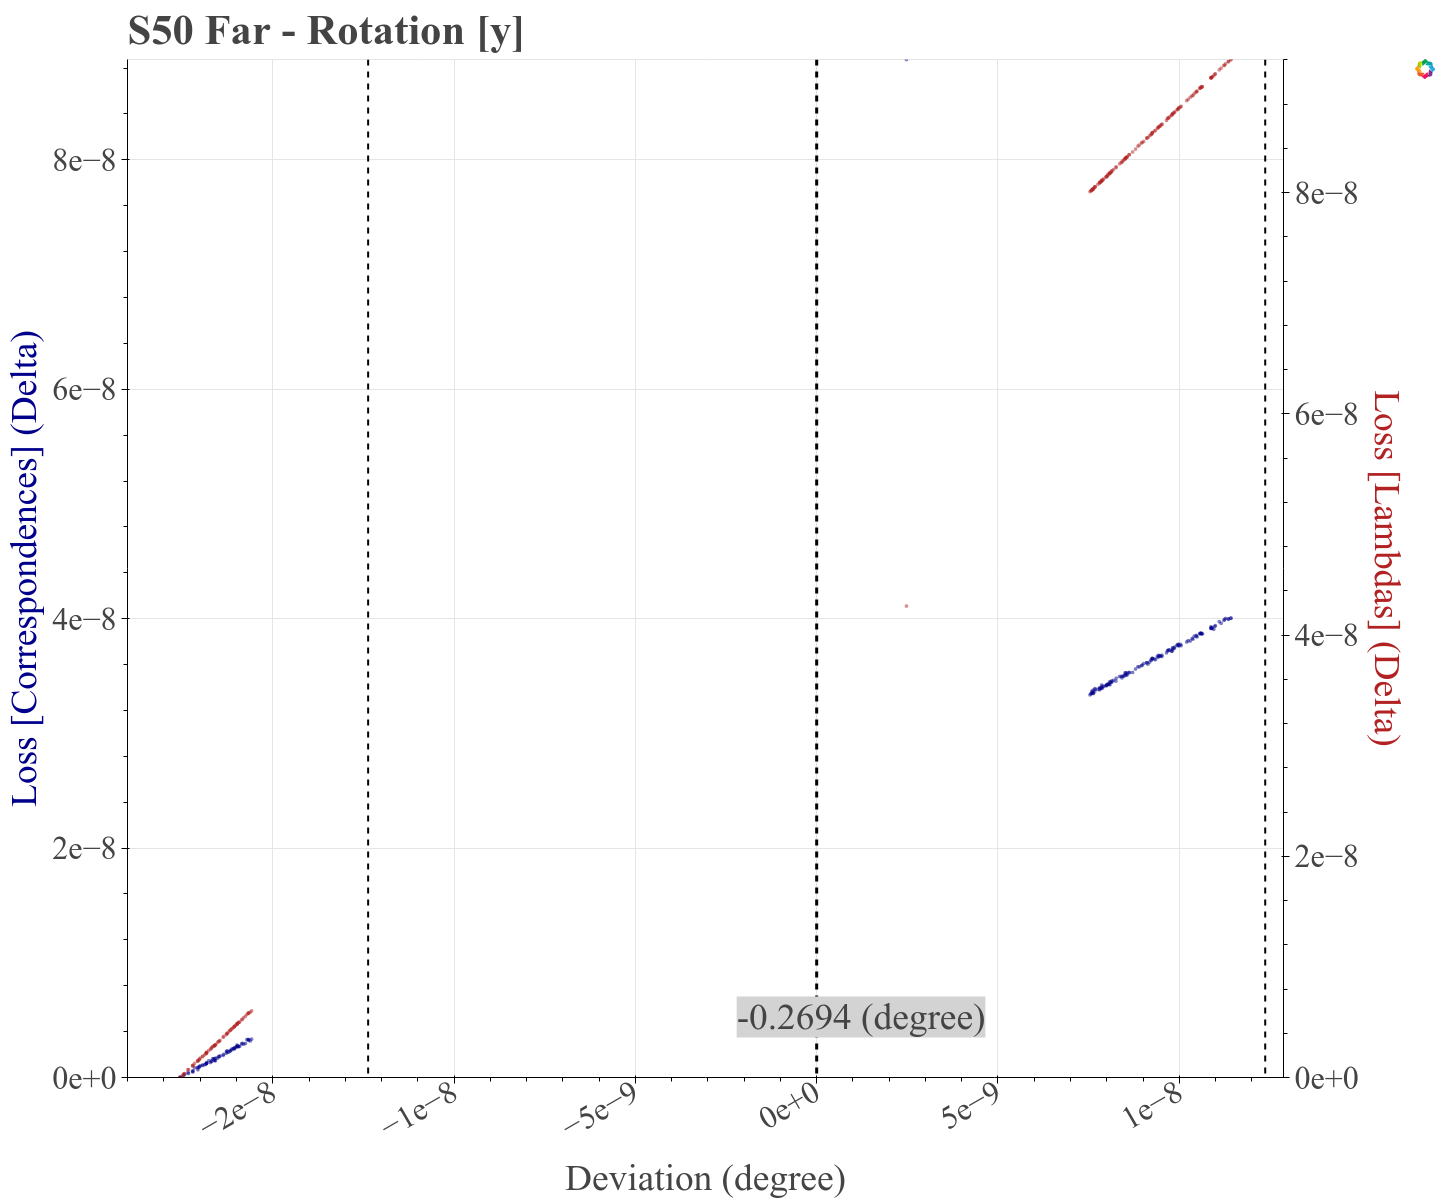
\includegraphics[width=0.45 \linewidth]{diagrams/calibration/s50_s_far/parameters.csv/Rotation[y]_vs_Loss[Correspondences]_vs_Loss[Lambdas]_cluster_All.png} \\
    
    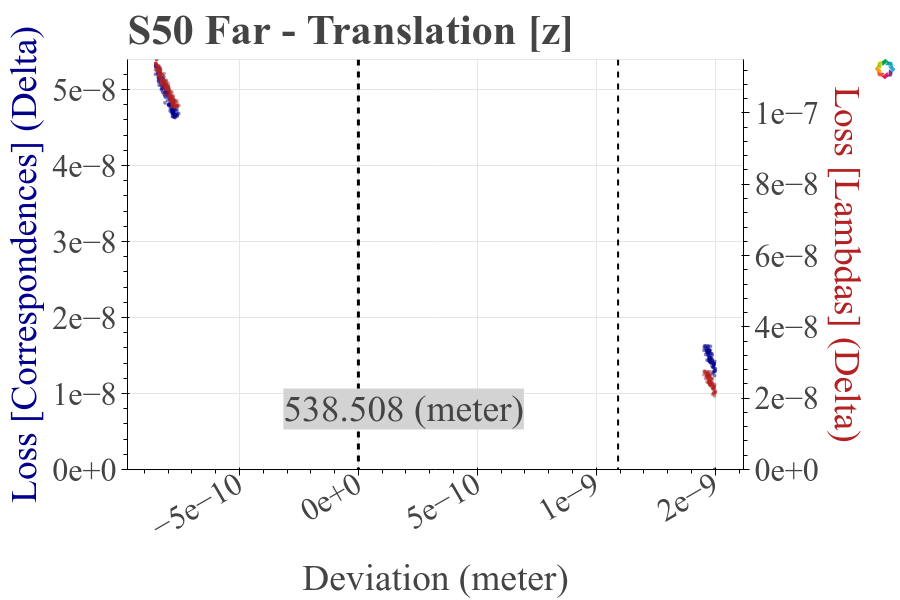
\includegraphics[width=0.45 \linewidth]{diagrams/calibration/s50_s_far/parameters.csv/Translation[z]_vs_Loss[Correspondences]_vs_Loss[Lambdas]_cluster_All.png} &
    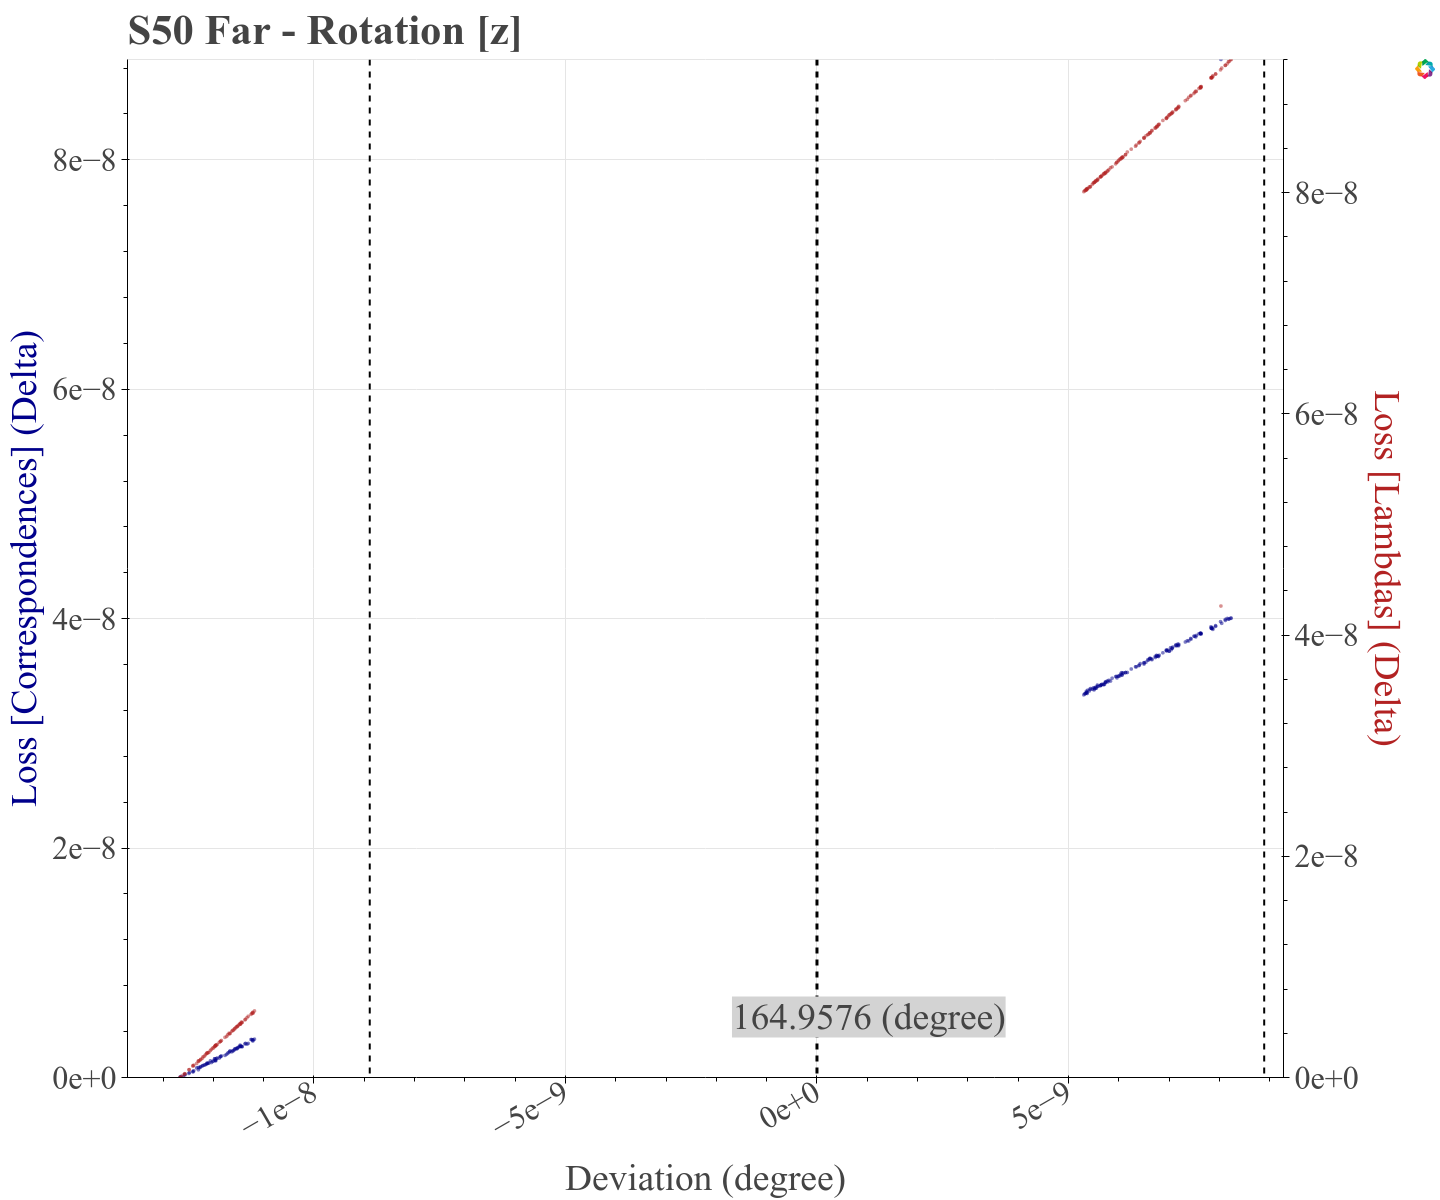
\includegraphics[width=0.45 \linewidth]{diagrams/calibration/s50_s_far/parameters.csv/Rotation[z]_vs_Loss[Correspondences]_vs_Loss[Lambdas]_cluster_All.png} \\

    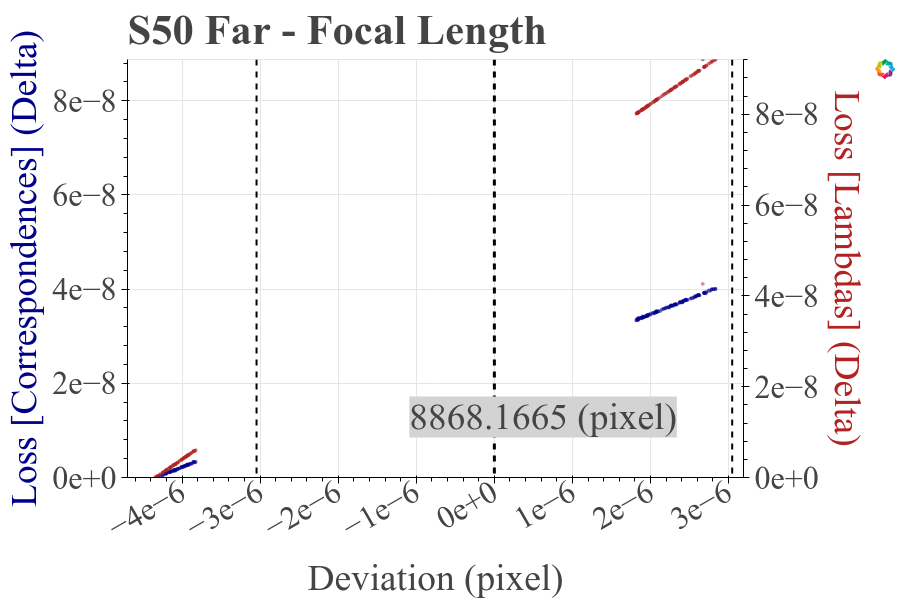
\includegraphics[width=0.45 \linewidth]{diagrams/calibration/s50_s_far/parameters.csv/FocalLength_vs_Loss[Correspondences]_vs_Loss[Lambdas]_cluster_All.png} &

  \end{tabular}
\caption{
  Camera: \camsf{5}.
  Left: The resulting translational parameters plotted against the remaining losses. 
  Right: The resulting rotational parameters plotted against the remaining losses.
  Bottom: The resulting focal length  plotted against the remaining losses.
    }
\label{fig:static_calibration_algorithmic_error_s50_s_far}
\end{figure*}

\begin{figure*}[!ht]
  \centering
  \begin{tabular}{cc}
    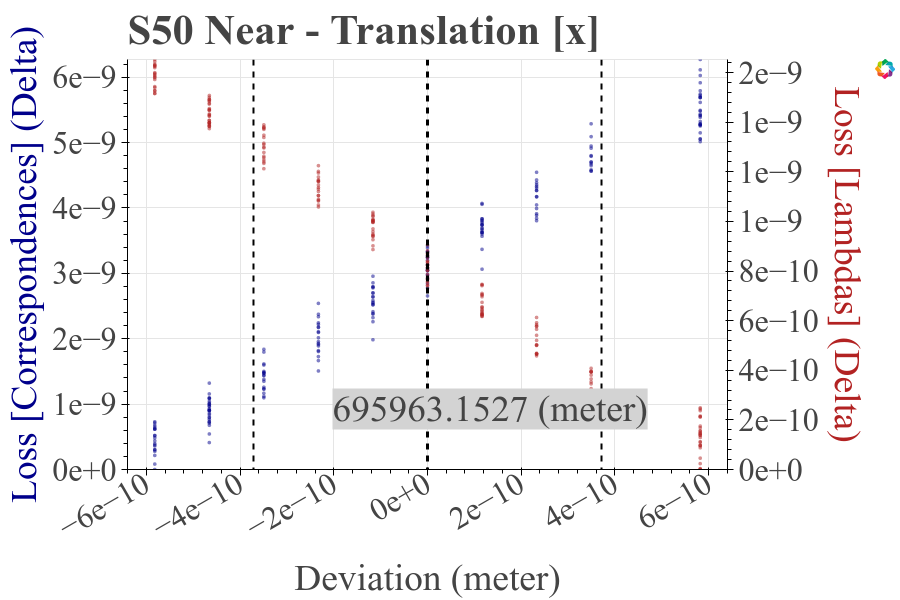
\includegraphics[width=0.45 \linewidth]{diagrams/calibration/s50_s_near/parameters.csv/Translation[x]_vs_Loss[Correspondences]_vs_Loss[Lambdas]_cluster_All.png} &
    \includegraphics[width=0.45 \linewidth]{diagrams/calibration/s50_s_near/parameters.csv/Rotation[x]_vs_Loss[Correspondences]_vs_Loss[Lambdas]_cluster_All.png} \\
    
    \includegraphics[width=0.45 \linewidth]{diagrams/calibration/s50_s_near/parameters.csv/Translation[y]_vs_Loss[Correspondences]_vs_Loss[Lambdas]_cluster_All.png} &
    \includegraphics[width=0.45 \linewidth]{diagrams/calibration/s50_s_near/parameters.csv/Rotation[y]_vs_Loss[Correspondences]_vs_Loss[Lambdas]_cluster_All.png} \\
    
    \includegraphics[width=0.45 \linewidth]{diagrams/calibration/s50_s_near/parameters.csv/Translation[z]_vs_Loss[Correspondences]_vs_Loss[Lambdas]_cluster_All.png} &
    \includegraphics[width=0.45 \linewidth]{diagrams/calibration/s50_s_near/parameters.csv/Rotation[z]_vs_Loss[Correspondences]_vs_Loss[Lambdas]_cluster_All.png} \\

    \includegraphics[width=0.45 \linewidth]{diagrams/calibration/s50_s_near/parameters.csv/FocalLength_vs_Loss[Correspondences]_vs_Loss[Lambdas]_cluster_All.png} &
\end{tabular}
\caption{
  Camera: \camsn{5}.
  Left: The resulting translational parameters plotted against the remaining losses. 
  Right: The resulting rotational parameters plotted against the remaining losses.
  Bottom: The resulting focal length  plotted against the remaining losses.
     }
\label{fig:static_calibration_algorithmic_error_s50_s_near}
\end{figure*}
